\documentclass[twoside,makeidx]{book}
%\usepackage{fancyhdr}%
\usepackage[T1]{fontenc}
\usepackage[utf8]{inputenc}
\usepackage{xspace}
\usepackage{xcolor}
\usepackage{combelow}
\usepackage{newunicodechar}
\newunicodechar{ș}{\cb{s}}
\newunicodechar{ț}{\cb{t}}

%% \usepackage{fontspec,xunicode,xltxtra}
%% \setromanfont[Mapping=tex-text]{Times}
%% \setsansfont[Mapping=tex-text]{Lucida Grande} 
%% \setmonofont{Courier New}

\definecolor{orange}{HTML}{DA4F3A}

\usepackage{pdfpages}

%\usepackage{draftwatermark}
%\SetWatermarkText{DRAFT...}
%\SetWatermarkScale{0.8}
%\SetWatermarkLightness{0.9}

% set paper size and margins; needs to be adapted for A5 ideally, we
% should have a document class for conference handbooks where A5
% vs. letter-halved is a class option
\usepackage[
  paperheight=8.75in, 
  paperwidth=5.75in, 
  inner=.75in,
  outer=.5in,
  bottom=.75in,
  top=.75in,
  twoside]{geometry}

% Lots of macros
\usepackage[T1]{fontenc}
\usepackage{hyperref}
\usepackage[utf8]{inputenc}
\usepackage{textcomp}
\usepackage{scrextend}
\usepackage{graphicx}
\usepackage{color}
\definecolor{mygray}{gray}{0.75}
\usepackage{colortbl}
\usepackage{fancyhdr}
\usepackage[Bjornstrup]{fncychap}
\usepackage{longtable}
\usepackage{tabularx}
\usepackage{lscape}
\usepackage{array}
\usepackage{calc}
\usepackage{csquotes}
\usepackage[american]{babel}
\usepackage{multicol}
\usepackage{multirow}
\usepackage{times}
\usepackage{helvet}
\usepackage[maxnames=25,minnames=3,babel=hyphen]{biblatex}
\usepackage{bibentry}
\usepackage{setspace}
\usepackage{ifthen}
\usepackage{pstricks}
\usepackage{rotating}
\usepackage{makeidx}
\usepackage{marginnote}
\usepackage{ragged2e}
\usepackage{mathpazo}
\usepackage{graphbox}
\usepackage{booktabs}

%\providecommand{\BIBand}{and}

\newcommand{\leftheader}{}  
\newcommand{\rightheader}{} 
\pagestyle{fancy}
  % header spec
  %\renewcommand{\headrule}{{\color[rgb]{0.696,0,0}% 
  %\renewcommand{\headrule}{{\color[rgb]{0.132,0.125,.46}% 
  \renewcommand{\headrule}{{\color[HTML]{b12008}% 
    \hrule height 2pt width \headwidth}
    \vspace{1pt}%
    {\color{mygray}%
    \hrule height 1pt width \headwidth
  \vspace{-4pt}}}

  \fancyhf{}				       % clear header contents
  %\fancyhead[LE]{\textit{\nouppercase{\leftmark}}}
  %\fancyhead[RO]{\textit{\nouppercase{\rightmark}}} % define header contents
  \fancyhead[LE]{\textit{\nouppercase{\leftheader}}}
  \fancyhead[RO]{\textit{\nouppercase{\rightheader}}} % define header contents

  % footer spec
  \renewcommand{\footrule}{\hrule width \headwidth height 1mm\vskip\footruleskip}
  \renewcommand{\footruleskip}{0.5\normalbaselineskip}
  \fancyfoot[C]{\thepage}			 %define footer conten
%
%  \rfoot{\setlength{\unitlength}{1mm} % logo in right part of footer
%  \begin{picture}(0,0)
    %\put(-13,-10){\includegraphics[scale=0.3]{images/conf.jpg}}%
%    \put(-10,-5){\includegraphics[scale=0.2]{images/conf.jpg}}%
%  \end{picture}}

\makeatletter
\renewcommand\chapter{\if@openright\cleardoublepage\else\clearpage\fi %let headers/footers show on pages that start a chapter
                    \global\@topnum\z@
                    \@afterindentfalse
                    \secdef\@chapter\@schapter}

\renewcommand{\chaptermark}[1]{\markboth{#1}{}} % show chapter in header w/o numbering
\renewcommand{\sectionmark}[1]{\markright{#1}{}} % show section in headers w/o numbering

% redefine sections to have a horizontal rule and no numbering
\def\section{\@ifstar\unnumberedsection\numberedsection}
\def\numberedsection{\@ifnextchar[%]
  \numberedsectionwithtwoarguments\numberedsectionwithoneargument}
\def\unnumberedsection{\@ifnextchar[%]
  \unnumberedsectionwithtwoarguments\unnumberedsectionwithoneargument}
\def\numberedsectionwithoneargument#1{\numberedsectionwithtwoarguments[#1]{#1}}
\def\unnumberedsectionwithoneargument#1{\unnumberedsectionwithtwoarguments[#1]{#1}}
\def\numberedsectionwithtwoarguments[#1]#2{
  \ifhmode\par\fi
  \removelastskip
  \vskip 3ex\goodbreak
  \refstepcounter{section}%			   % increment counter
  \begingroup
  \noindent\begin{minipage}{\columnwidth}
  \leavevmode\Large\bfseries\raggedright
%  \thesection\  % leave out numbering
  #2 \par\nobreak
  \vskip -.5em
  \noindent\hrulefill\nobreak
  \end{minipage}
  \endgroup
  \vskip 1ex\nobreak
  \markright{#1}{} % add mark to right (secondary) header
  \addcontentsline{toc}{section}{%
%    \protect\numberline{\thesection}% % leave out number
    #1}%
  }
\def\unnumberedsectionwithtwoarguments[#1]#2{
  \ifhmode\par\fi
  \removelastskip
  \vskip 3ex\goodbreak
  \begingroup
  \noindent\begin{minipage}{\columnwidth}
  \leavevmode\Large\bfseries\raggedright
  #2\par\nobreak
  \vskip -.5em
  \noindent\hrulefill\nobreak
  \end{minipage}
  \endgroup
  \vskip 1ex\nobreak
  \markright{#1}{} % add mark to right (secondary) header
  }

% redefine subsections to have a horizontal rule and no numbering
\def\subsection{\@ifstar\unnumberedsubsection\numberedsubsection}
\def\numberedsubsection{\@ifnextchar[%]
  \numberedsubsectionwithtwoarguments\numberedsubsectionwithoneargument}
\def\unnumberedsubsection{\@ifnextchar[%]
  \unnumberedsubsectionwithtwoarguments\unnumberedsubsectionwithoneargument}
\def\numberedsubsectionwithoneargument#1{\numberedsubsectionwithtwoarguments[#1]{#1}}
\def\unnumberedsubsectionwithoneargument#1{\unnumberedsubsectionwithtwoarguments[#1]{#1}}
\def\numberedsubsectionwithtwoarguments[#1]#2{
  \ifhmode\par\fi
  \removelastskip
  \vskip 3ex\goodbreak
  \refstepcounter{subsection}%			   % increment counter
  \begingroup
  \noindent
  \leavevmode\normalsize\bfseries\raggedright
%  \thesubsection\  % leave out numbering
  #2 \par\nobreak
  \endgroup
  \vskip 1ex\nobreak
  \addcontentsline{toc}{subsection}{%
%    \protect\numberline{\thesubsection}% % leave out number
    #1}%
  }
\def\unnumberedsubsectionwithtwoarguments[#1]#2{
  \ifhmode\par\fi
  \removelastskip
  \vskip 3ex\goodbreak
  \begingroup
  \noindent
  \leavevmode\normalsize\bfseries\raggedright
  #2\par\nobreak
  \endgroup
  \vskip 1ex\nobreak
  }

\makeatother

% Clears to an even-numbered page
\def\clearevenpage{
     \clearpage 
     \ifodd\value{page} \hbox{}\newpage\fi
}

% Clears to the back-cover (for logos)
\def\cleartobackcover{
     \clearpage 
     \ifodd\value{page}\pagestyle{empty}\clearevenpage \else\hbox{}\cleardoublepage\pagestyle{empty}\clearevenpage\fi
}

%\renewcommand{\cleardoublepage}{\clearpage}

% Min: index
\makeindex

%\raggedbottom
%\setlength{\parindent}{0pt}
% Unicode issues
% \DeclareUnicodeCharacter{fi}{fi}

% Min: correct column widths
\newlength{\mycolumnwidth}
\setlength{\mycolumnwidth}{\columnwidth}
\addtolength{\mycolumnwidth}{-2ex}

\renewcommand{\textfraction}{.2}
\renewcommand{\bottomfraction}{.8}

\newenvironment{bio}
               {\begin{figure}[b]
                   \centerline{\rule{.5\linewidth}{.5pt}}\vspace{2ex}
                   \setlength{\parskip}{1ex}\setlength{\parindent}{0ex}}
               {\end{figure}}

\setlength{\parindent}{1em}

\fancypagestyle{emptyheader}
{
  \fancyhf{}
  \fancyfoot[C]{\thepage}
}

\newcommand{\setheaders}[2]{%
  \renewcommand{\leftheader}{#1}%
  \renewcommand{\rightheader}{#2}}
%%%%%%%%%%%%%%%%%%%%%%%%%%%%%%%%%%%%%%%%%%%%%%%%%%
 
% Macros for the production of Conference Handbooks / Program Brochures from
% ACLPUB bundles from the START conference manager.

\newlength{\w}      % width of the space available for paper entries in a
                    % multi-track schedule
\newlength{\tsl}    % with of a time specification in a schedule
\newlength{\en}     % \en-space
%\newlength{\tmplen}

\setlength{\tabcolsep}{.5ex} 

\newenvironment{SingleTrackSchedule}%
{%
  \settowidth{\en}{--}
  \setlength{\w}{\linewidth}%
  \settowidth{\tsl}{$\,$} % temporary abuse of this length measure
  \addtolength{\w}{-2\tsl}%
  \settowidth{\tsl}{00:00}
  \addtolength{\w}{-2\tsl}%
  \addtolength{\w}{-2\tabcolsep}%
  \addtolength{\w}{-1\en}%
  \begin{longtable}{@{}%
      >{\raggedleft}p{\tsl}%
      @{$\,$}%
      p{1\en}%
      @{$\,$}%
      >{\raggedright}p{\tsl}%
      >{\RaggedRight}p{\w}@{}}%
}{%
  \end{longtable}%
}

\newenvironment{TwoTrackSchedule}{
\settowidth{\en}{--}
\setlength{\w}{\linewidth}%
\settowidth{\tsl}{$\,$}
\addtolength{\w}{-2\tsl}%
\settowidth{\tsl}{\footnotesize 00:00am}
\addtolength{\tsl}{2ex}
\addtolength{\w}{-2\tsl}%
\addtolength{\w}{-2\tabcolsep}%
\addtolength{\w}{-1\en}%
\addtolength{\w}{-1cm}%
\renewcommand{\arraystretch}{1.1}
%\setlength{\tmplen}{\tabcolsep}
%\addtolength{\tmplen}{-.5\arrayrulewidth}
\begin{longtable}{@{}|%
    >{\raggedleft}p{\tsl}%
    @{$\,$}%
    p{1\en}%
    @{$\,$}%
    >{\raggedright}%
    p{\tsl}|%
    >{\centering\arraybackslash}p{.5\w}|%
    >{\centering\arraybackslash}p{.5\w}|@{}}%
}{\end{longtable}}

\newenvironment{ThreeTrackSchedule}{
\settowidth{\en}{--}
\setlength{\w}{\linewidth}%
\settowidth{\tsl}{$\,$}
\addtolength{\w}{-2\tsl}%
\settowidth{\tsl}{00:00am}
\addtolength{\tsl}{2ex}
\addtolength{\w}{-2\tsl}%
\addtolength{\w}{-2\tabcolsep}%
\addtolength{\w}{-1\en}%
\addtolength{\w}{-1cm}%
\renewcommand{\arraystretch}{1.1}
%\setlength{\tmplen}{\tabcolsep}
%\addtolength{\tmplen}{-.5\arrayrulewidth}
\begin{longtable}{@{}%
    >{\raggedleft}p{\tsl}%
    @{$\,$}%
    p{1\en}%
    @{$\,$}%
    >{\raggedright}%
    p{\tsl}|%
    >{\centering\arraybackslash}p{.333\w}|%
    >{\centering\arraybackslash}p{.333\w}|%
    >{\centering\arraybackslash}p{.333\w}@{}}%
}{\end{longtable}}

\newenvironment{FourTrackSchedule}{
\settowidth{\en}{--}
\setlength{\w}{\linewidth}%
\settowidth{\tsl}{$\,$}
\addtolength{\w}{-2\tsl}%
\settowidth{\tsl}{00:00am}
\addtolength{\tsl}{2ex}
\addtolength{\w}{-2\tsl}%
\addtolength{\w}{-2\tabcolsep}%
\addtolength{\w}{-1\en}%
\addtolength{\w}{-1cm}%
\renewcommand{\arraystretch}{1.1}
%\setlength{\tmplen}{\tabcolsep}
%\addtolength{\tmplen}{-.5\arrayrulewidth}
\begin{longtable}{@{}|%
    >{\raggedleft}p{\tsl}%
    @{$\,$}%
    p{1\en}%
    @{$\,$}%
    >{\raggedright}%
    p{\tsl}|%
    >{\centering\arraybackslash}p{.25\w}|%
    >{\centering\arraybackslash}p{.25\w}|%
    >{\centering\arraybackslash}p{.25\w}|%
    >{\centering\arraybackslash}p{.25\w}|@{}}%
}{\end{longtable}}

%%%%%%%%%%% BreakTime Macro %%%%%%%%%%%%%%%%%%%%%%%%%%%%%%%%%%%%%%%%%%%%%%
\newcommand{\BreakTime}[4]{%
% adds a gray background to a break or a break-style event
% #1 start time
% #2 end   time
% #3 number of parallel tracks
% #4 label of the break or break-style event
\multicolumn{3}{c}{\cellcolor[gray]{.8}} & 
\multicolumn{#3}{c}{\cellcolor[gray]{.8}} \\[-3ex]\hline 
\bfseries #1 & -- & \bfseries #2 &
\multicolumn{#3}{c|}{\bfseries #4}}
%%%%%%%%%%%%%%%%%%%%%%%%%%%%%%%%%%%%%%%%%%%%%%%%%%%%%%%%%%%%%%%%%%%%%%%%%%

%%%%%%%%%%% PlenaryEvent Macro %%%%%%%%%%%%%%%%%%%%%%%%%%%%%%%%%%%%%%%%%%%%%%
\newcommand{\PlenaryEvent}[4]{%
% event with nothing else going on in parallel
\bfseries #1 & -- & \bfseries #2 &
\multicolumn{#3}{>{\centering\arraybackslash}p{\w}|@{}}{\bfseries #4}}
%%%%%%%%%%%%%%%%%%%%%%%%%%%%%%%%%%%%%%%%%%%%%%%%%%%%%%%%%%%%%%%%%%%%%%%%%%

%%%%%%%%%%% SessionHeader Macro %%%%%%%%%%%%%%%%%%%%%%%%%%%%%%%%%%%%%%%%%%%%%%
\newcommand{\SingleTrackSessionHeader}[3]{%
% event with nothing else going on in parallel
\ifthenelse{\equal{{#1}}{{}}}{&}{#1 & -- } & #2 
\ifthenelse{\equal{#1}{{}}}{}{\hfill}
&\multicolumn{1}{>{\raggedright\arraybackslash}m{\w}}{\bfseries #3}}
%%%%%%%%%%%%%%%%%%%%%%%%%%%%%%%%%%%%%%%%%%%%%%%%%%%%%%%%%%%%%%%%%%%%%%%%%%

% insert references to the page ranges 
\newcommand{\ppp}[1]{pp. \pageref{#1start}--\pageref{#1end}}

% the following code requires the biblatex package
\DeclareNameFormat{authorswithinitials}{%
  % name format that prints the list of authors with initals
  \ifcase\value{uniquename}%
    \usebibmacro{name:first-last}{#1}{#4}{#5}{#7}%
  \or
    \ifuseprefix
      {\usebibmacro{name:first-last}{#1}{#4}{#5}{#8}}
      {\usebibmacro{name:first-last}{#1}{#4}{#6}{#8}}%
  \or
    \usebibmacro{name:first-last}{#1}{#4}{#5}{#7}%
  \fi
  \usebibmacro{name:andothers}}

\DeclareNameFormat{authorlastnames}{%
  % name format that prints the list of author last names
  \ifcase\value{uniquename}%
    \usebibmacro{name:last}{#1}{#4}{#5}{#7}%
  \or
    \ifuseprefix
      {\usebibmacro{name:last}{#1}{#4}{#5}{#8}}
      {\usebibmacro{name:last}{#1}{#4}{#6}{#8}}%
  \or
    \usebibmacro{name:last}{#1}{#4}{#5}{#7}%
  \fi
  \usebibmacro{name:andothers}}

\DeclareNameFormat{fullauthornames}{%
  % name format that prints the list of authors with full author names
  \ifcase\value{uniquename}%
    \usebibmacro{name:first-last}{#1}{#3}{#5}{#7}%
    \or
    \ifuseprefix
        {\usebibmacro{name:first-last}{#1}{#3}{#5}{#8}}
        {\usebibmacro{name:first-last}{#1}{#3}{#6}{#8}}%
  \or
  \usebibmacro{name:first-last}{#1}{#3}{#5}{#7}%
  \fi
  \usebibmacro{name:andothers}}

% insert the list of authors with first name initials
\DeclareCiteCommand{\citeauthorslastnamesonly}{%
  \boolfalse{citetracker}%
  \boolfalse{pagetracker}%
  \usebibmacro{prenote}%
}{\ifciteindex{\indexnames{labelname}}{}%
  \printnames[authorlastnames]{labelname}%
}{\multicitedelim}{\usebibmacro{postnote}}

% insert the list of authors with first name initials
\DeclareCiteCommand{\citeauthorswithinitials}{%
  \boolfalse{citetracker}%
  \boolfalse{pagetracker}%
  \usebibmacro{prenote}%
}{\ifciteindex{\indexnames{labelname}}{}%
  \printnames[authorswithinitials]{labelname}%
}{\multicitedelim}{\usebibmacro{postnote}}
  
% insert the list of authors with full names
\DeclareCiteCommand{\citefullauthornames}{%
  \boolfalse{citetracker}%
  \boolfalse{pagetracker}%
  \usebibmacro{prenote}%
}{%\ifciteindex{\indexnames{labelname}}{}%
  \indexnames{labelname}%
  \printnames[fullauthornames]{labelname}%
}{\multicitedelim}{\usebibmacro{postnote}}
                     
\DeclareFieldFormat[inproceedings]{citetitle}{#1}

\newcommand{\paperauthor}[1]{{\em #1}}
\newcommand{\papertitle}[1]{\citetitle{#1}}

% insert an entry into a multi-track schedule cell
\newcommand{\paperentry}[1]{%
  \renewcommand{\baselinestretch}{.8}%
  \setlength{\parindent}{0pt}%
    \begin{small}%
      \parbox[t]{\linewidth}{%
        {\em \papertitle{#1}}
        \vspace{.5ex}}\par%
      \vfill
      \parbox[b]{\linewidth}{\raggedright%
        \paperauthor{\citeauthorslastnamesonly{#1}}%
        %% \mbox{}~\dotfill~ {\bfseries p.~\pageref{#1}}
        }%
    \end{small}%
}

\newcommand{\sempaperentry}[1]{%
  &&$\bullet$&
  \parbox[t]{\linewidth}{\raggedright\papertitle{#1}\newline
  {\itshape\paperauthor{\citefullauthornames{#1}}}
\mbox{}~\dotfill~\pageref{#1}}}

\newcommand{\atpaperentry}[2]{%
  \footnotesize\parbox[t]{\linewidth}{\noindent%
    \makebox[0pt][r]{#1\hspace*{\tabcolsep}}{%
      \paperauthor{\citeauthorswithinitials{#2}}}:
    \papertitle{#2}\mbox{}~\dotfill{p.~\pageref{#2}\par}}}

% insert an entry into a poster session index
\newcommand{\posterentry}[1]{%
  \renewcommand{\baselinestretch}{1.2}%
  \settowidth{\w}{\bfseries p.~\pageref{#1}}%
  \addtolength{\w}{1em}%
  \parbox[t]{\linewidth-\w}{\noindent\raggedright{\bfseries\papertitle{#1}}%
    \linebreak[0]\ {---~{\paperauthor{\citeauthorswithinitials{#1}}}}\mbox{}~\dotfill\makebox[0pt][l]%
    {\makebox[\w][r]{\bfseries p.~\pageref{#1}}}\vspace{1em}\par}}

% insert an abstract into a list of abstracts (for posters, no time needed)
\newcommand{\posterabstract}[1]{%
  \noindent%
  \begin{minipage}{\linewidth}%
    \label{#1}%
          {\bfseries\normalsize\papertitle{#1}}\\
          \normalsize\paperauthor{\citefullauthornames{#1}}
  \end{minipage}\vspace{1mm}\\\nopagebreak%
  \noindent{\small\input{auto/abstracts/#1}}\par}

% insert an abstract into a list of abstracts
\newcommand{\paperabstract}[5]{%
  % #1 day
  % #2 time
  % #3 session title
  % #4 location
  % #5 paper id
  \noindent%
  \begin{minipage}{\linewidth}%
    \label{#5}%
      %\rule{\linewidth}{1pt}\linebreak
          {\bfseries\normalsize\papertitle{#5}} \\
          \hfill\normalsize\paperauthor{\citefullauthornames{#5}}
%      {\small #1 #2 --- #4}\vspace{.5ex}\\
          \hfill {\small #2}
%    \parbox[t]{.8\linewidth}{\centering
%      {\bfseries\papertitle{\citetitle{#5}}}\linebreak
%      \paperauthor{\citefullauthornames{#5}}}%
%    \parbox[t]{.2\linewidth}{\raggedleft\small%
%      #1\linebreak #2\linebreak #4}\par\nopagebreak
  %% \begin{center}\label{#5}%
  %%   \sloppy\hyphenpenalty=0%
  %%   %{\small --- Session: #3 --- \vspace{.5em}}\linebreak		% Redundant info? - B
  %%   {\bfseries \citetitle{#5}} \vspace{.5em}\linebreak
  %%   {\itshape    \citefullauthornames{#5}}%\vspace{.5em}\linebreak	% Reduce space between header and abstract - B
  %%   %#1 #2 --- #4\linebreak 						% Redundant info? - B
  \end{minipage}\vspace{1mm}\\\nopagebreak%
  \noindent{\small\input{auto/abstracts/#5}}\par}

\newcommand{\TutorialCoverPage}[4]{%
\vspace*{.25in}
% #1 Tutorial Number
% #2 Tutorial Title
% #3 Tutorial Presenter
% #4 Tutorial Presenter Information
%\begin{minipage}{\linewidth}
\begin{centering}
\includegraphics[height=7.5cm,clip=true]{content/fmatter/conference-logo.eps}\\

\vspace{.5cm}

{\Large
The 2012 Conference of the \linebreak
North American Chapter of the \linebreak
Association for Computational Linguistics: \linebreak
Human Language Technologies}\par

\vspace{3cm}

%\begin{tabular}{@{}>{\centering\arraybackslash}p{.7\linewidth}@{}}
\centerline{\huge\bfseries Tutorial~#1\vspace{.25em}}
{\Large Tutorial Notes}\\

\vspace{1cm}

\begin{minipage}{.7\linewidth}
\centering\Large%\setstretch{1.1}
{\bfseries#2}
\end{minipage}

\vfill

{\itshape\Large #3}\\[.5em]
{#4}\\
\vspace{1cm}

{June 3, 2012}\\
{Montr\'{e}al, Queb\'{e}c, Canada}\\\end{centering}
%\end{minipage}
\clearpage}

\newcommand{\STARSEM}{$^\ast$SEM}

\newcommand{\nix}{\cellcolor{mygray}}
% used for the room occupation tables in the local information section

\newcommand{\mrup}[2]{\multirow{#1}{*}{%
%\rotatebox[origin=c]{90}{#2}}%
\begin{sideways}#2\end{sideways}%
}}

\newcommand{\PaperInSchedule}[4][false]{%
  % #1 (optional) with or without a \pageref to the abstract
  % #2 start time (can be empty)
  % #3 end time (can be empty)
  % #4 paper id
  \ifthenelse{\equal{{#2}}{{}}}{&&\hfill}{#2&--&} % ... start time
  \ifthenelse{\equal{{#3}}{{}}}{$\bullet$}{#3}    %   ... end time
    & \parbox[t]{\linewidth}{\raggedright\papertitle{#4}\newline
      {\paperauthor{\citefullauthornames{#4}}}%
      \ifthenelse{\equal{#1}{true}}{\mbox()~\dotfill~\pageref{#4}}}}

\newcommand{\ScheduleItem}[4][false]{%
  % #1 (optional) with or without a \pageref to the abstract
  % #2 start time (can be empty)
  % #3 end time (can be empty)
  % #4 paper id
  \ifthenelse{\equal{{#2}}{{}}}{&&\hfill}{#2&--&} % ... start time
  \ifthenelse{\equal{{#3}}{{}}}{$\bullet$}{#3}    %   ... end time
    & \parbox[t]{\linewidth}{\raggedright\papertitle{#4}\newline
      {\paperauthor{\citefullauthornames{#4}}}%
      \ifthenelse{\equal{#1}{true}}{\mbox()~\dotfill~\pageref{#4}}}}

\newenvironment{singledaywsprogram}[5]{%
% #1 worshop id
% #2 workshop number
% #3 workshop title
% #4 workshop day
% #5 workshop venue
\section{\textbf{W~#2:} #3}\label{#1}

\begin{center}
{\bfseries\Large #4}\vspace{1em}\par
{\itshape Venue:} #5\vspace{0.75em}\par
{\large\bfseries Program\vspace{0.75em}}\par
\setlength{\w}{\linewidth}
\begin{SingleTrackSchedule}}%
{\end{SingleTrackSchedule}\end{center}}

%% WORKSHOP SCHEDULE %%%%%%%%%%%%%%%%%%%%%%%%%%%%%%%%%%%%%%%%%%%%

%\newlength{\wsscheduleindentation}
%\newlength{\wsschedulelabelwidth}
\newenvironment{wsschedule}[5]{%
  % #1 workshop title
  % #2 workshop number
  % #3 workshop label
  % #4 workshop paper ID
  % #5 workshop location
  %\addcontentsline{toc}{section}{{{\bfseries W~#2:} #4}}

  %\addcontentsline{toc}{section}{{{\bfseries W~#2:} 
  %    \ifthenelse{\equal{#1}{none}}{#4}{#1}}}

  % For workshops numbered 0, don't prepend W0 on the contents page
  \clearpage
  \ifthenelse{\equal{#2}{0}}
             {\section{\textbf{#1}}}
             {\section[{\bfseries W#2:} #1]{{\bfseries Workshop #2:} #1}}
             %% {{\addcontentsline{toc}{section}{{#1}}}}
             %% {{\addcontentsline{toc}{section}{{{\bfseries W#2:} #1}}}}

  \markboth{}{}
  \label{#3}
  \begin{center}
%    {\huge{\Large Workshop #2:}\vspace{.5ex}\\
    %% {\Large
    %%   \ifthenelse{\equal{#2}{0}}{{}}{{\huge{Workshop #2:\\\vspace{.5ex}}}}
    %%   #1\par}
    {\ifthenelse{\equal{#4}{0}}{{}}{{Organizers: \paperauthor{\citefullauthornames{#4}}}\par}}
    {\large Venue: #5 \vspace{2em}}\\
    %% {\huge Workshop Program\vspace{1ex}}
  \end{center}
  \markright{{\bfseries W~#2:} #1}{}%
  \begin{list}{{}}{%
      \settowidth{\labelwidth}{\bfseries 12:00pm--12:00pm}
      \setlength{\labelsep}{1ex}
      \setlength{\topsep}{0pt}
      \setlength{\parsep}{0pt}
      \setlength{\listparindent}{0pt}
      \setlength{\itemsep}{.5ex}
      \setlength{\rightmargin}{0pt}
      \setlength{\leftmargin}{\labelwidth}
      \addtolength{\leftmargin}{\labelsep}}
}{\end{list}}

\newcounter{WorkshopCounter}

\newenvironment{tutorial}[4]{%
  \stepcounter{TutorialCounter}
  % #1 short title
  % #2 tutorial bibtex ID
  % #3 date and time
  % #4 location

  % Cannot get \papertitle to expand
  \section[\textbf{T\theTutorialCounter:} {#1}]{Tutorial \theTutorialCounter}
  \begin{center}
    \begin{Large}
      \bfseries \papertitle{#2}\\ \vspace{2em}\par
    \end{Large}
    {\itshape \tutorialauthors{#2}}\vspace{1em}\par
    #3 \vspace{1em}\\
    #4
  \end{center}}

\newcounter{TutorialCounter}

\newcommand{\tutorialauthors}[1]{
    \paperauthor{\citefullauthornames{#1}}}

\newcommand{\wspaperentry}[1]{
  \parbox[t]{\linewidth}{\raggedright\papertitle{#1}\newline
    \paperauthor{\citefullauthornames{#1}}}}

\newcommand{\sessionchair}[2]{
  \emph{Chair: #1 #2}\par\index{#2, #1}}

\newcommand{\papertitleandauthor}[1]{
  {\bfseries \papertitle{#1}}\\
  \paperauthor{\citefullauthornames{#1}}}

\newcommand{\papertableentry}[1]{
  {\papertitle{#1}}\newline
  {\paperauthor{\citeauthorslastnamesonly{#1}}}}

\newenvironment{SessionOverview}[7]{
  \section[#1]{#1 Overview -- #2}
  \setheaders{#1}{#2}
  \begin{center}
    \righthyphenmin2
    \sloppy
    \begin{tabular}{>{\RaggedRight}p{0.8in}|>{\RaggedRight}p{0.8in}|>{\RaggedRight}p{0.8in}|>{\RaggedRight}p{0.8in}|>{\RaggedRight}p{0.8in}}
      \bf Track A & \bf Track B & \bf Track C & \bf Track D & \bf Track E \\
      \it #3 & \it #4 & \it #5 & \it #6 & \it #7 \\
      \TrackALoc & \TrackBLoc & \TrackCLoc & \TrackDLoc & \TrackELoc \\
      \hline\hline}
{\end{tabular}\end{center}}

\newenvironment{ThreeSessionOverview}[5]{
  \section[#1]{#1 Overview -- #2}
  \setheaders{#1}{#2}
  \begin{center}
    \righthyphenmin2
    \sloppy
    \begin{tabular}{|>{\RaggedRight}p{1.3in}|>{\RaggedRight}p{1.3in}|>{\RaggedRight}p{1.3in}|}
      \hline
      \bf Track A & \bf Track B & \bf Track C \\\hline
      \it #3 & \it #4 & \it #5 \\
      \TrackALoc & \TrackBLoc & \TrackCLoc \\
      \hline\hline}
{\hline\end{tabular}\end{center}}

\newcommand{\daydate}{DAY, DATE}
\newcommand{\daydateyear}{DAY, DATE, YEAR}
\newcommand{\setdaydateyear}[3]{
  \renewcommand{\daydateyear}{#1, #2, #3\xspace}
  \renewcommand{\daydate}{#1, #2\xspace}}
  
\newenvironment{linez}
 {\trivlist\nopagebreak
  \parindent0pt
%  \vspace{3pt}%
%  \hrule
%  \vspace{-3pt}%
  \item\relax\obeylines}
 {\par
  \nopagebreak
%  \vspace{3pt}%
%  \hrule
%  \vspace{3pt}%
  \endtrivlist}

\newcommand\todo[1]{\textcolor{red}{#1}}    

%% defines macros for event venues

% 2015 NAACL Venues

\newcommand{\TrackALoc}{\mbox{Funen}}
\newcommand{\TrackBLoc}{\mbox{Sealand}}
\newcommand{\TrackCLoc}{\mbox{Jutland}}

\newcommand{\BreakfastLoc}{\mbox{TODO NOT AVAILABLE}}
\newcommand{\BreakLoc}{\mbox{Foyer}}
\newcommand{\RegistrationLoc}{Foyer}

\newcommand{\UnknownLoc}{TBD}

\newcommand{\PlenaryLoc}{\mbox{Jutland}}
\newcommand{\PosterSessionLoc}{Foyer}
\newcommand{\StudentLunchLoc}{TODO}
\newcommand{\BusinessMeetingLoc}{\mbox{\PlenaryLoc}}
\newcommand{\OMMLoc}{\PlenaryLoc}
\newcommand{\SocialEventLoc}{\mbox{Øksnehallen Courtyard}}
\newcommand{\LunchLoc}{\mbox{}}

\newcommand{\SrwLoc}{\PosterSessionLoc}
\newcommand{\PosterLoc}{\PosterSessionLoc}
\newcommand{\DemoLoc}{\PosterSessionLoc}

\newcommand{\SocialLoc}{\SocialEventLoc}
\newcommand{\BusinessLoc}{\BusinessMeetingLoc}    % business meeting
\newcommand{\NaaclLoc}{\BusinessMeetingLoc}    % business meeting

\newcommand{\InvitedLoc}{\PlenaryLoc}
\newcommand{\BestLoc}{\PlenaryLoc}
\newcommand{\WelcomeLoc}{\PlenaryLoc}
\newcommand{\WelcomeReceptionLoc}{CPH Conference, Room \textit{Østerbro}}
\newcommand{\OneLoc}{\PlenaryLoc}  % one minute madness

% Tutorials
\newcommand{\TutLocA}{\mbox{TODO}}
\newcommand{\TutLocB}{\mbox{TODO}}
\newcommand{\TutLocC}{\mbox{TODO}}
\newcommand{\TutLocD}{\mbox{TODO}}
\newcommand{\TutLocE}{\mbox{TODO}}
\newcommand{\TutLocF}{\mbox{TODO}}
\newcommand{\TutLocG}{\mbox{todo}}
    
% *SEM location
\newcommand{\StarSEMLoc}{\mbox{TODO}}
\newcommand{\SemEvalLoc}{\mbox{TODO}}

% Workshop locations
\newcommand{\WShopLocA}{\mbox{TODO}}
\newcommand{\WShopLocB}{\mbox{TODO}}
\newcommand{\WShopLocC}{\mbox{TODO}}
\newcommand{\WShopLocD}{\mbox{TODO}}
\newcommand{\WShopLocE}{\mbox{TODO}}
\newcommand{\WShopLocF}{\mbox{TODO}}
\newcommand{\WShopLocG}{\mbox{TODO}}
\newcommand{\WShopLocH}{\mbox{TODO}}
\newcommand{\WShopLocI}{\mbox{TODO}}
\newcommand{\WShopLocJ}{\mbox{TODO}}
\newcommand{\WShopLocK}{\mbox{TODO}}
\newcommand{\WShopLocL}{\mbox{TODO}}
\newcommand{\WShopLocM}{\mbox{TODO}}
\newcommand{\WShopLocN}{\mbox{TODO}}
\newcommand{\WShopLocO}{\mbox{TODO}}



    % macros for event locations
% define macros for session titles here
\newcommand{\DDP}{Discourse, Dialog\linebreak[0] and Pragmatics}
\newcommand{\MT}{Machine\linebreak[0] Translation}
\newcommand{\IE}{Information\linebreak[0] Extraction}
\newcommand{\SLP}{Spoken Language\linebreak[0] Processing}
\newcommand{\ML}{Machine\linebreak[0] Learning}
\newcommand{\LRE}{Language Resources\linebreak[0] and Evaluation}
\newcommand{\PM}{Phonology and Morphology}
\newcommand{\SM}{Semantics}
\newcommand{\SP}{Syntax and Parsing}
\newcommand{\DC}{Discourse}
\newcommand{\CTM}{Document Categorization\linebreak[0] and Topic Modeling}
\newcommand{\SU}{Summarization}
\newcommand{\SSM}{Sentiment and\linebreak[0] Social Media}
%
\newcommand{\MonBEtitle}{\DDP~I}
\newcommand{\MonBWtitle}{\MT~I}
\newcommand{\MonBDtitle}{\IE~I}
%
\newcommand{\MonCEtitle}{\SLP}
\newcommand{\MonCWtitle}{\ML~I}
\newcommand{\MonCDtitle}{\LRE}

\newcommand{\MonBEloc}{\EBR}
\newcommand{\MonBWloc}{\WBR}
\newcommand{\MonBDloc}{\DBR}
\newcommand{\MonCEloc}{\EBR}
\newcommand{\MonCWloc}{\WBR}
\newcommand{\MonCDloc}{\DBR}

\newcommand{\TueDtitle}{Best Paper Awards}
\newcommand{\TueDloc}{\WCBR}

\newcommand{\TueEEtitle}{\PM}
\newcommand{\TueEEloc}{\EBR}
\newcommand{\TueECtitle}{\MT~II}
\newcommand{\TueECloc}{\CBR}
\newcommand{\TueEWtitle}{\SM~I}
\newcommand{\TueEWloc}{\WBR}
\newcommand{\TueEDtitle}{\SP}
\newcommand{\TueEDloc}{\DBR}

\newcommand{\TueFEtitle}{Short papers:\linebreak[0] \DC}
\newcommand{\TueFEloc}{\WBR}
\newcommand{\TueFCtitle}{Short papers:\linebreak[0] \MT}
\newcommand{\TueFCloc}{\CBR}
\newcommand{\TueFWtitle}{Short papers:\linebreak[0] \CTM}
\newcommand{\TueFWloc}{\WBR}
\newcommand{\TueFDtitle}{Short papers:\linebreak[0] Syntax}
\newcommand{\TueFDloc}{\DBR}

\newcommand{\WedGEtitle}{Short Papers: \SSM}
\newcommand{\WedGEloc}{\EBR}
\newcommand{\WedGCtitle}{Short Papers: \SM}
\newcommand{\WedGCloc}{\CBR}
\newcommand{\WedGWtitle}{Short Papers: \SU}
\newcommand{\WedGWloc}{\WBR}

\newcommand{\WedHEtitle}{\SSM}
\newcommand{\WedHEloc}{\EBR}
\newcommand{\WedHCtitle}{\ML~II}
\newcommand{\WedHCloc}{\CBR}
\newcommand{\WedHWtitle}{\DDP~II}
\newcommand{\WedHWloc}{\WBR}

\newcommand{\WedIEtitle}{\SU}
\newcommand{\WedIEloc}{\EBR}
\newcommand{\WedICtitle}{\SM~II}
\newcommand{\WedICloc}{\CBR}
\newcommand{\WedIWtitle}{\CTM~II}
\newcommand{\WedIWloc}{\WBR}
  % session titles and venues

\renewcommand{\normalsize}{\fontsize{8}{9}\selectfont}
\renewcommand{\small}{\fontsize{7}{8}\selectfont}
\renewcommand{\footnotesize}{\fontsize{6}{6}\selectfont}
\renewcommand{\large}{\fontsize{10}{11}\selectfont}
\renewcommand{\Large}{\fontsize{12}{14}\selectfont}
\renewcommand{\huge}{\fontsize{14}{17}\selectfont}

% for each part of the conference, add the .bib file produced with
% meta2bibtex.py here:

% MAIN CONFERENCE
\bibliography{auto/tacl/papers.bib}
\bibliography{auto/papers/papers.bib}
\bibliography{auto/demos/papers.bib}

% WORKSHOPS
% main workshop info (titles/organizers/...)
\bibliography{content/workshops/papers.bib}
% individual WS contributions
\bibliography{auto/argmining2017/papers.bib}
\bibliography{auto/bea2017/papers.bib}
\bibliography{auto/DiscoMT2017/papers.bib}
\bibliography{auto/GenNLP/papers.bib}
\bibliography{auto/NewSum/papers.bib}
\bibliography{auto/nlp-journ/papers.bib}
\bibliography{auto/repeval/papers.bib}
\bibliography{auto/sclem/papers.bib}
\bibliography{auto/scnlp/papers.bib}
\bibliography{auto/SPNLP/papers.bib}
\bibliography{auto/StyVa/papers.bib}
\bibliography{auto/wassa2017/papers.bib}
\bibliography{auto/wmt/papers.bib}
\bibliography{auto/w-nut/papers.bib}

% TUTORIALS
\bibliography{auto/tutorial-final/papers.bib}

%%%%%%%%%%%%%%%%%%%%%%%%%%%%%%%%%%%%%%%%%%%%%%%%%%%%%%%%%%%%%%%%%

\begin{document}

\setdaydateyear{Thursday}{September 7}{2017}

%% COVER %%%%%%%%%%%%%%%%%%%%%%%%%%%%%%%%%%%%%%%%%%%%%%%%%%%%%%%%

%\fancyfoot[C]{}
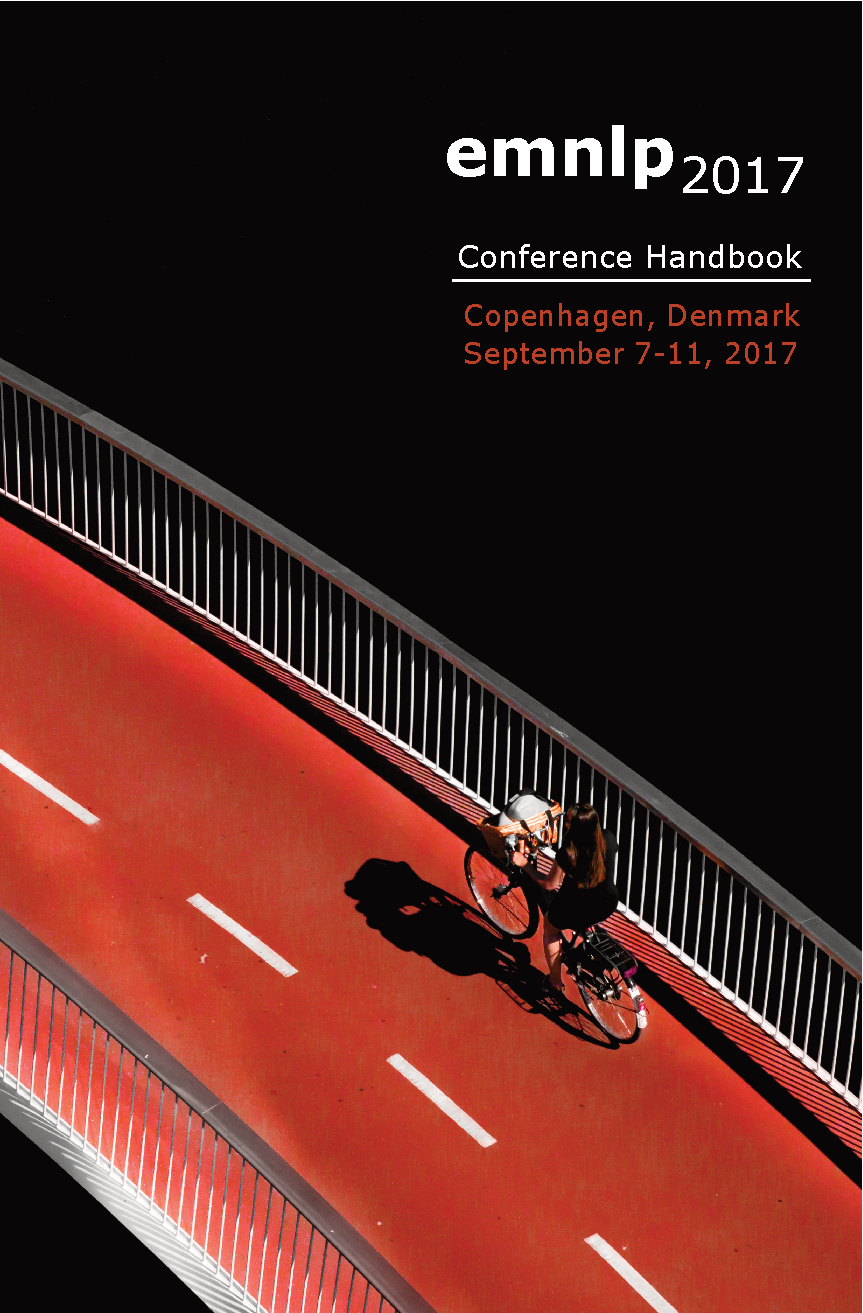
\includepdf[pages={1}]{content/fmatter/EMNLP17_cover.pdf}

%% INSIDE FRONT COVER %%%%%%%%%%%%%%%%%%%%%%%%%%%%%%%%%%%%%%%%%%%

\thispagestyle{empty}
\vspace*{6in}
\begin{linez}
\emph{Cover design by Aurelia Bunescu}\index{Bunescu, Aurelia}
\emph{Cover photo by Matthew James}\index{James, Matthew}
\emph{Deep gratitude to Matt Post for invaluable advice with creating this handbook}\index{Post, Matt}
\emph{Handbook assembled by Joachim Bingel}\index{Bingel, Joachim}
\emph{Printing by Frederiksbergs Bogtrykkeri A/S}
\end{linez}

%% \addcontentsline{toc}{section}{Hotel Maps}

%\thispagestyle{empty}
%\begin{center}
%  \begin{tabular}{r}
%    \includegraphics[width=3.8in]{content/venue-map.png} \\
%    \textbf{AREA PLAN}\\\hline
%    \textbf{LOBBY LEVEL}\\
%    \includegraphics[width=3.8in]{content/venue-map.png}
%  \end{tabular}
%\end{center}

\begin{figure}[p]
\centering
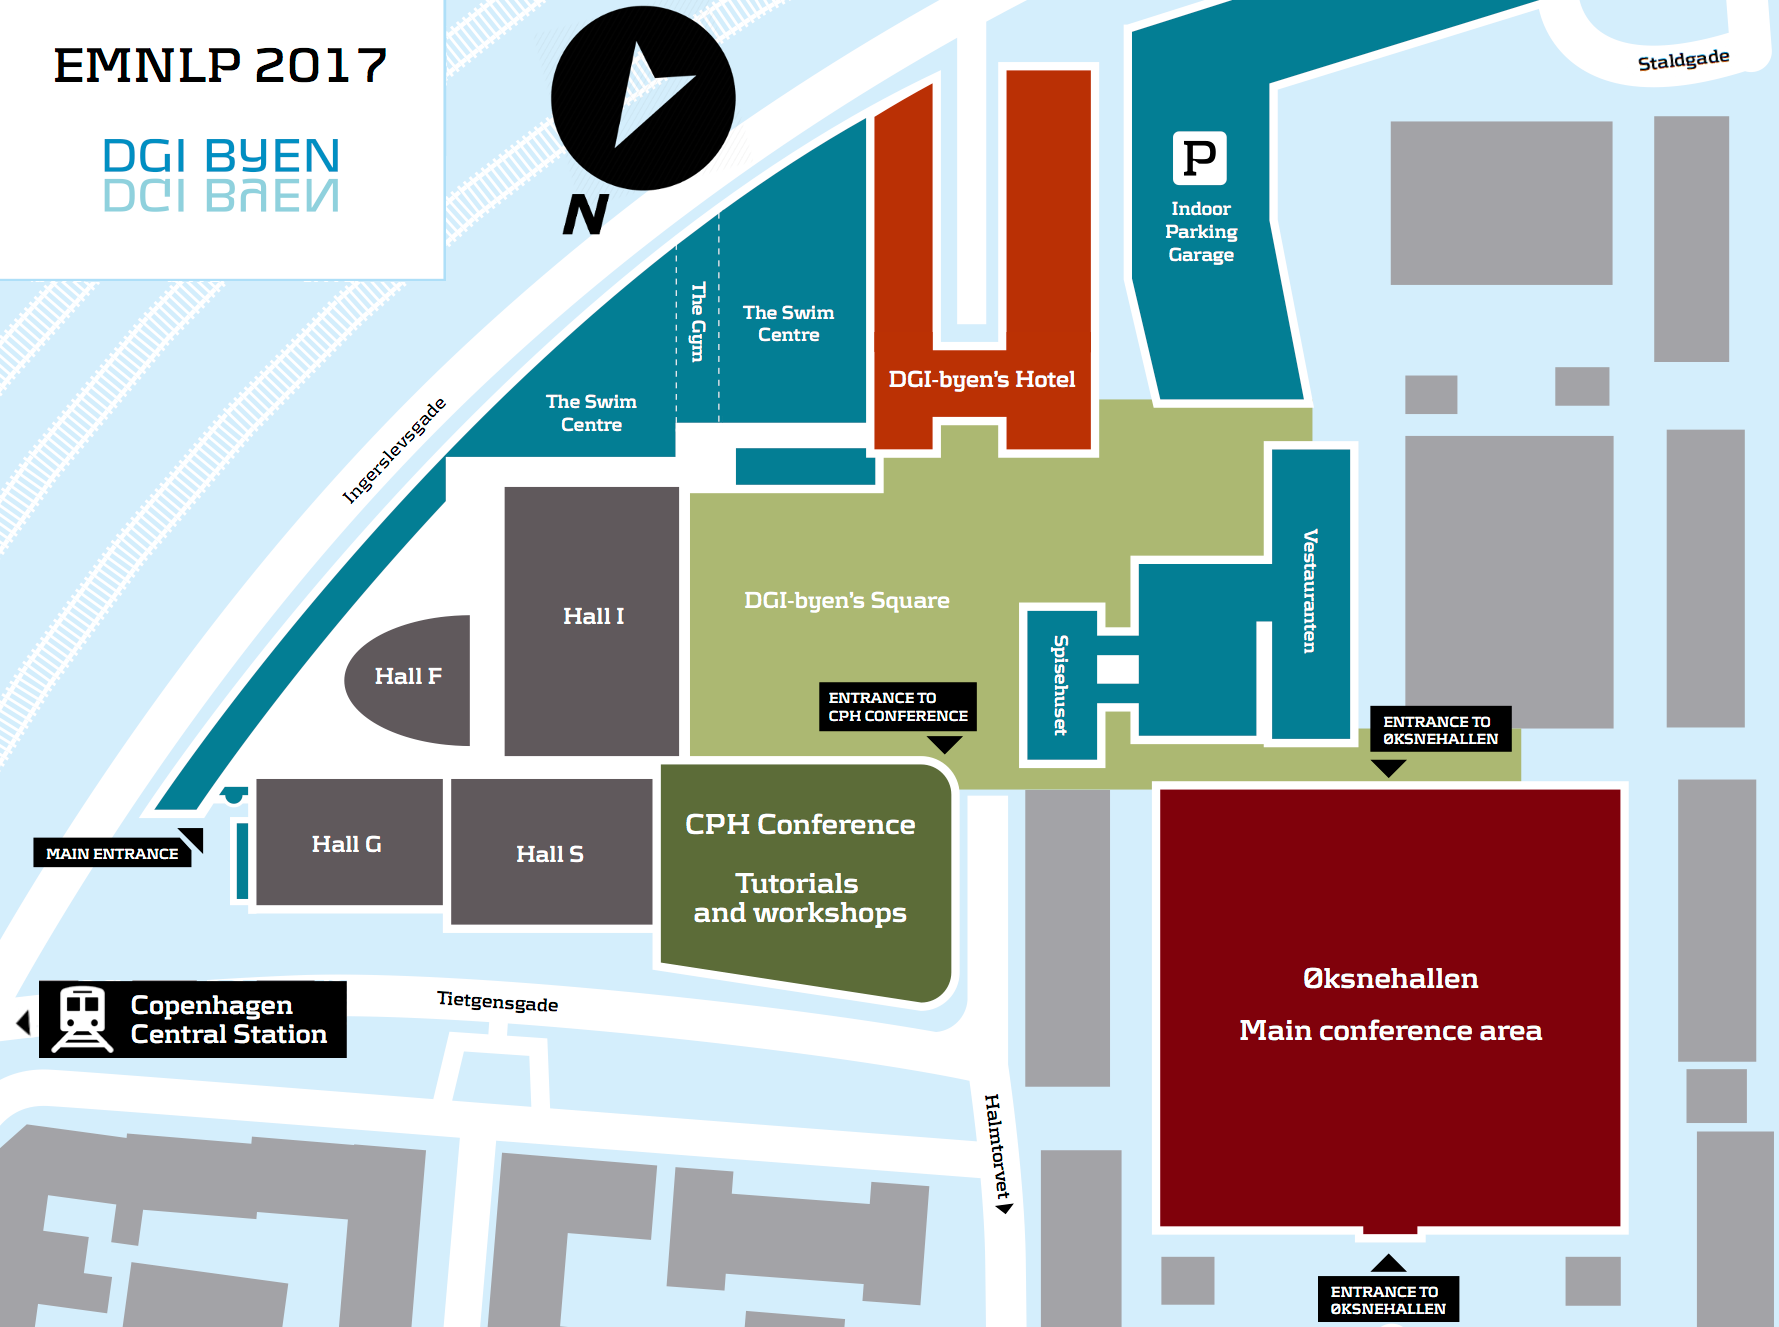
\includegraphics[height=\textwidth,angle=90,origin=c]{content/fmatter/venue_map_small.png}
%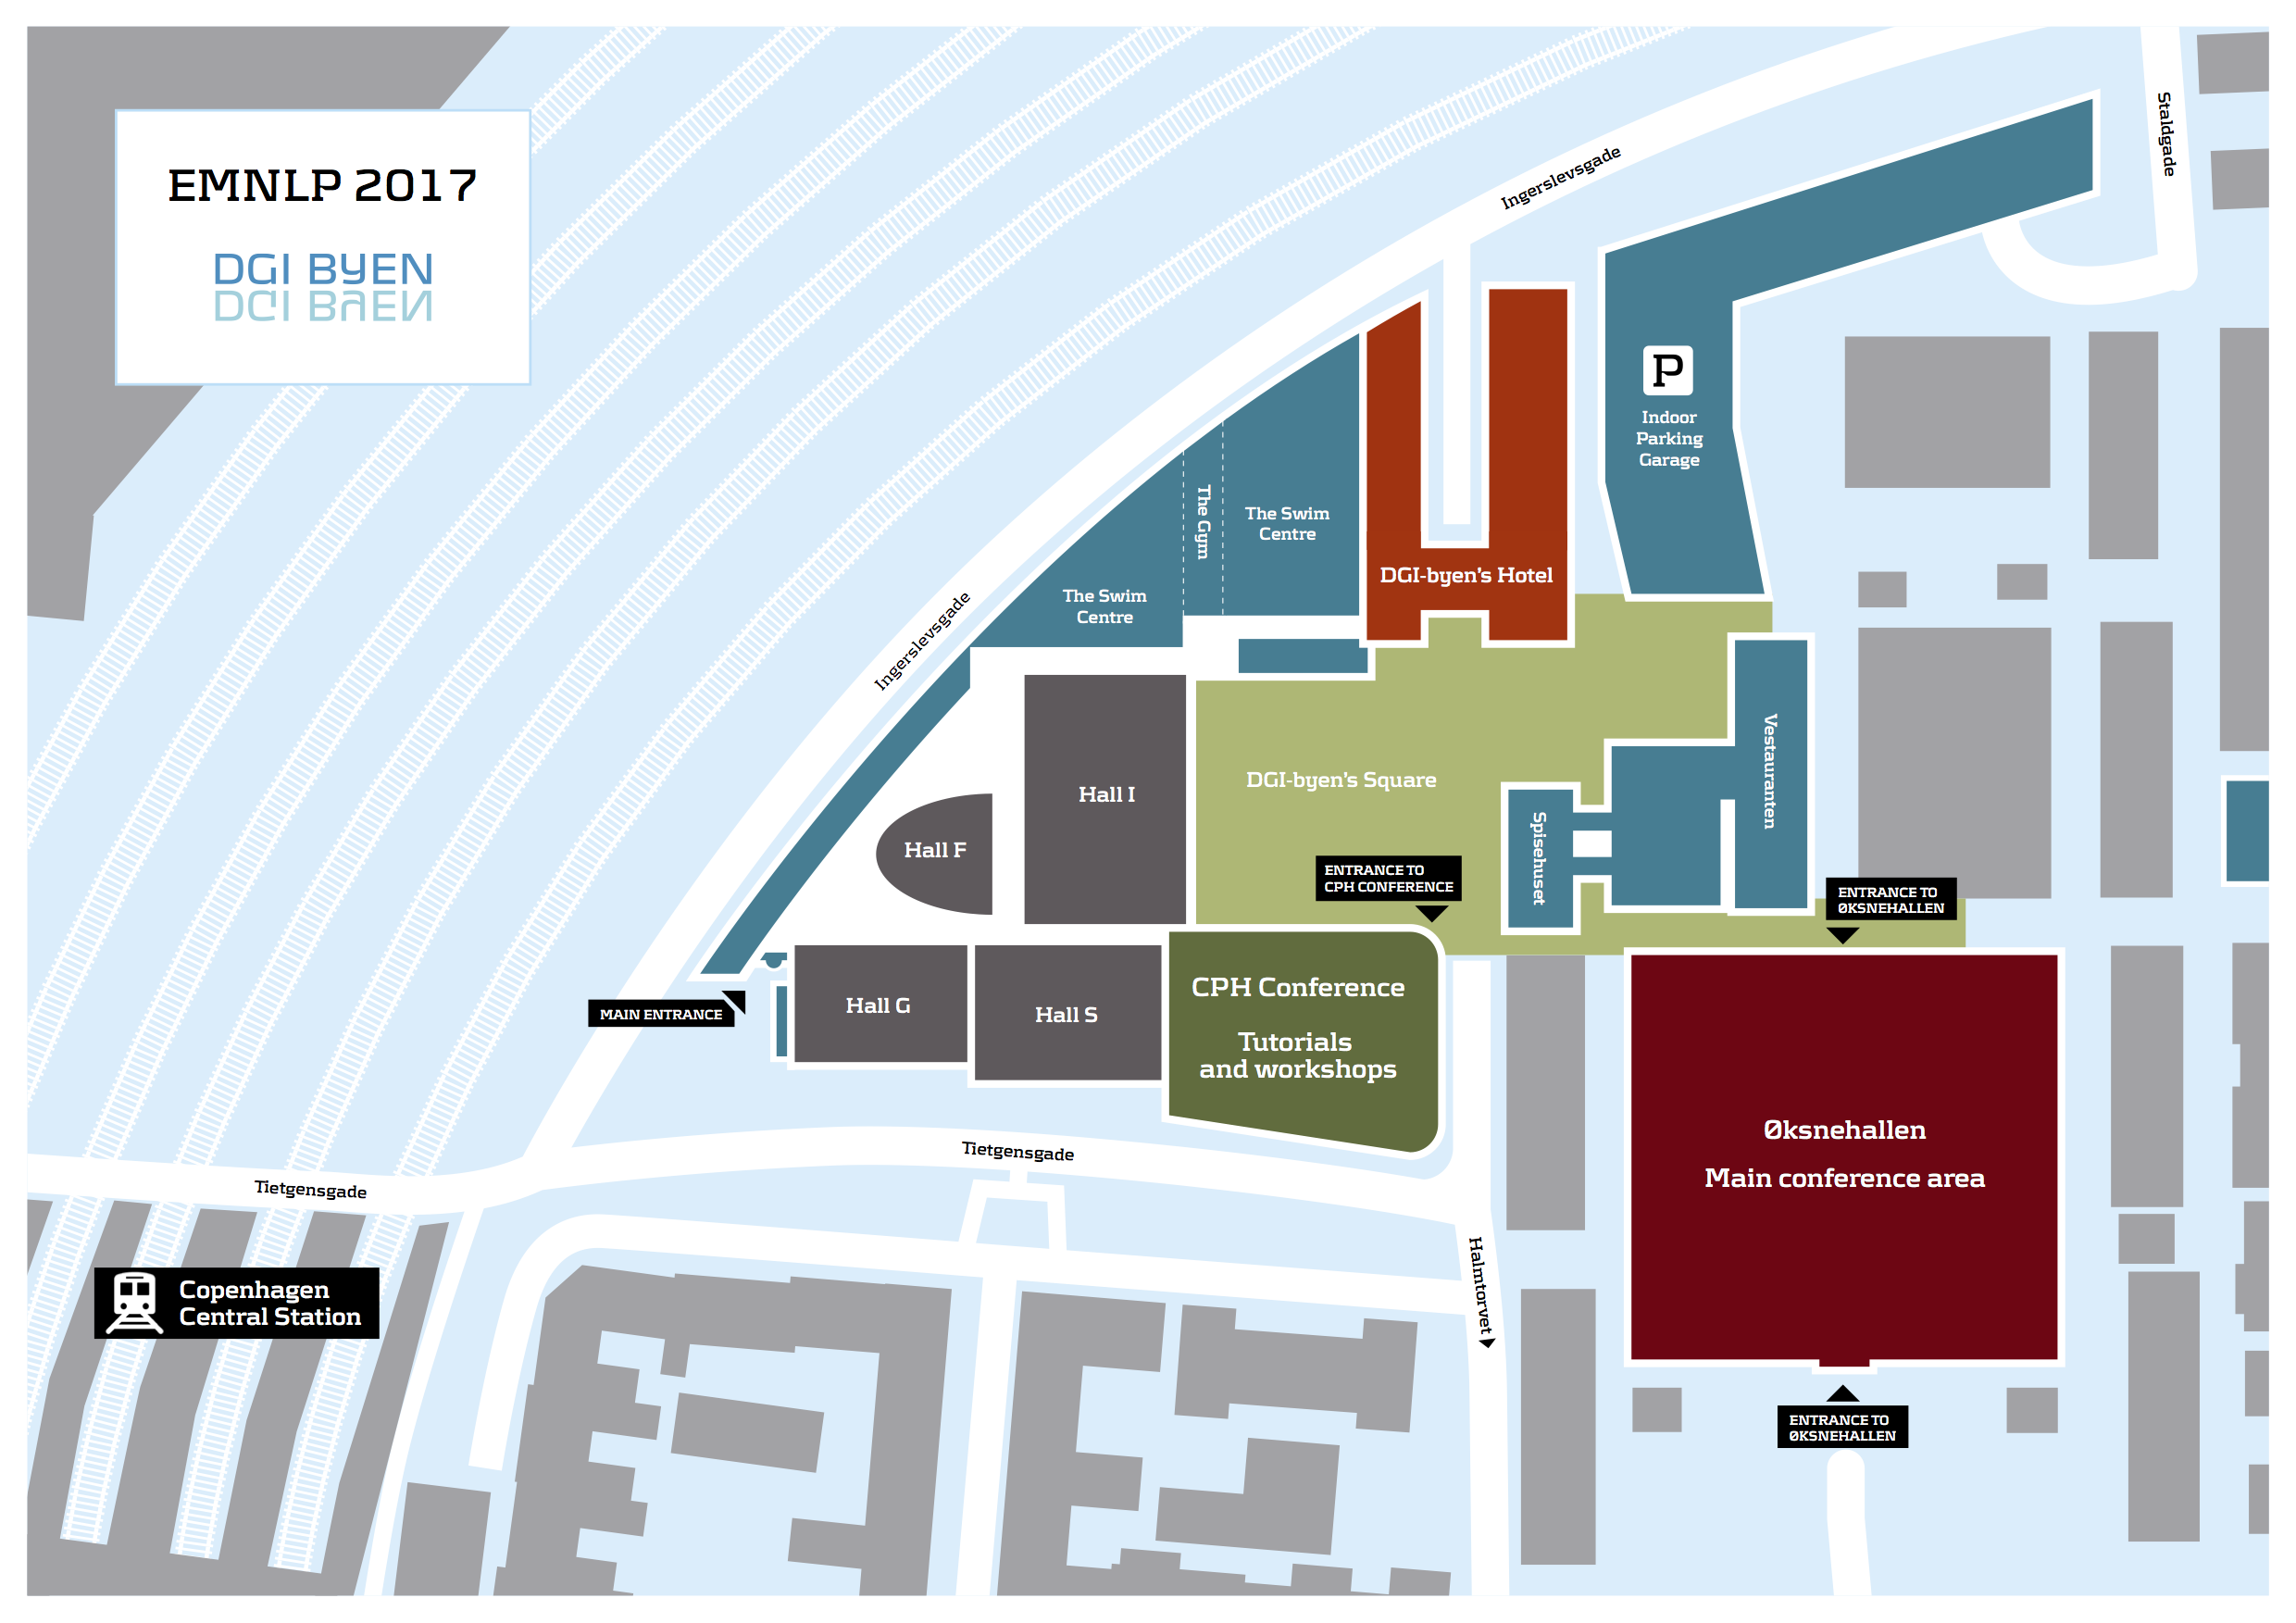
\includegraphics[width=7in,angle=90,origin=c]{content/venue_map.png}
\end{figure}

\begin{figure}[p]
\centering
\textbf{CPH Conference Floorplan}\\
(Most workshops, three tutorials)
\vspace{3em}
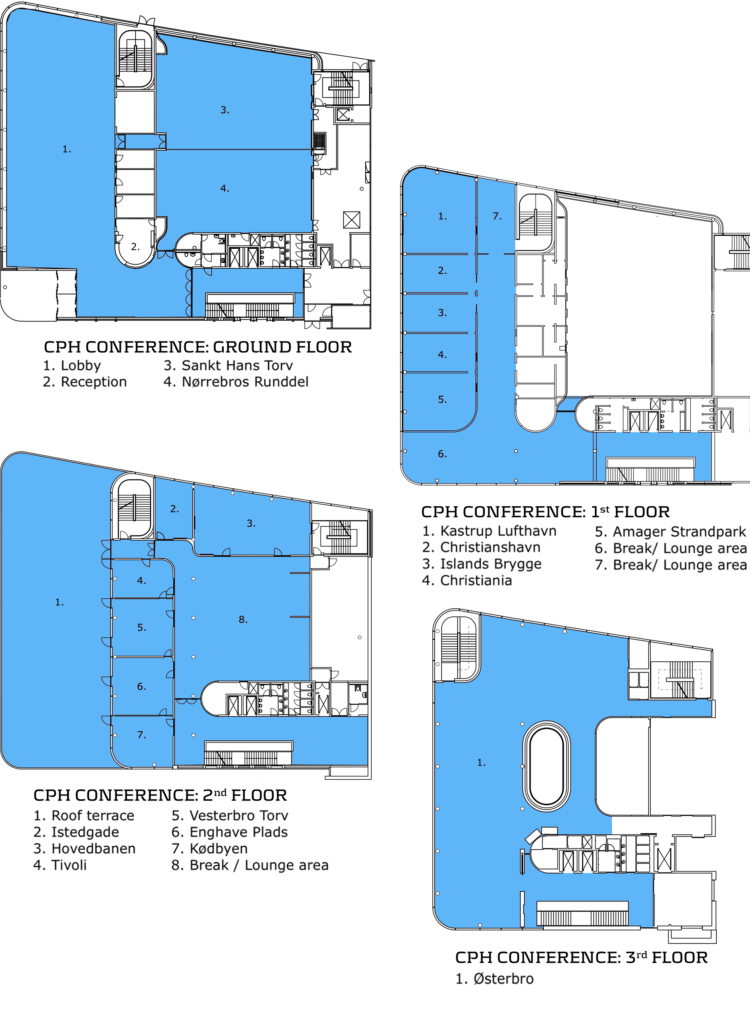
\includegraphics[width=\textwidth]{content/fmatter/floorplan_DGI_w_grid.pdf}
\end{figure}

\begin{figure}[p]
\centering
\textbf{Øksnehallen Floorplan}\\
(Main Conference, WMT, Tutorial 5)
\vspace{10em}
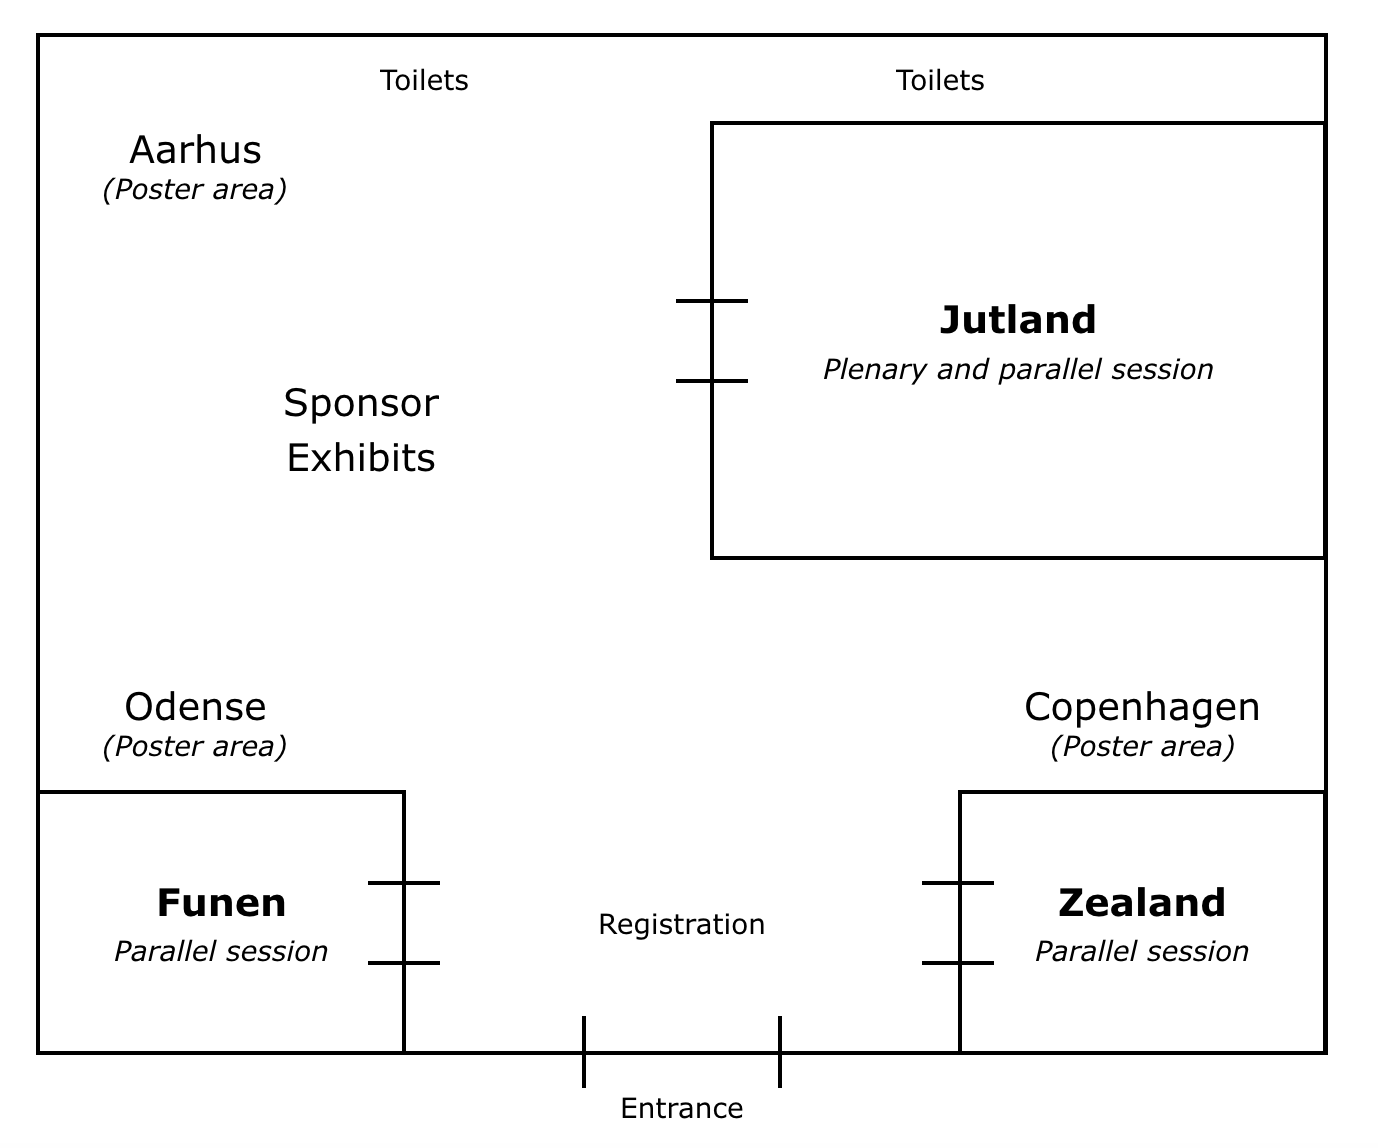
\includegraphics[width=\textwidth]{content/fmatter/floorplan_oeksnehallen.png}
\end{figure}

%\cleardoublepage

%\newpage
%\cleardoublepage
%\fancyfoot[C]{\thepage}
\frontmatter

%% TOC %%%%%%%%%%%%%%%%%%%%%%%%%%%%%%%%%%%%%%%%%%%%%%%%%%%%%%%%%%
\addcontentsline{toc}{chapter}{Table of Contents}
\setcounter{tocdepth}{2}
\tableofcontents
\mainmatter

%% PREFACE %%%%%%%%%%%%%%%%%%%%%%%%%%%%%%%%%%%%%%%%%%%%%%%%%%%%%%
\chapter{Conference Information}
\section{Message from the General Chair}\vspace{2em}
\setheaders%
    {Message from the General Chair}%
    {Message from the General Chair}
\thispagestyle{emptyheader}

\setlength{\parskip}{1ex}

Thank you so much for joining us in Copenhagen.  Welcome to a cosmopolitan city of fantastic restaurants, lovely seascapes, rich history, and lots and lots of cyclists! 

We have an exciting program lined up for you, with three invited talks, fifteen workshops, seven tutorials, nine TACL presentations, 323 reviewed papers presented as both oral talks and posters, and twenty-one demos.  I am especially grateful to our Program Chairs, Rebecca Hwa and Sebastian Riedel, who did a fantastic job managing a backbreaking 1,500 paper submissions (1466 reviewed papers).  This involved 51 Area chairs and 980 reviewers.  We tried some new things this year (never conducive to a smooth process) including a more careful handling of the COIs that result from Area Chair submissions, and the addition of a meta-review step to encourage more thoughtful reviewing.  We are soliciting feedback on the meta-review process, from both reviewers and authors.  Despite the additional time involvement, many of the Area Chairs embraced this new approach, and would like to repeat it. However, there are clearly a few dissenters, since Rebecca and Sebastian ended up writing around 200 meta-reviews themselves at the last minute.  We are also trying to raise the visibility and status of the poster sessions by integrating them as parallel sessions alongside oral talks, with poster session chairs.  This is in response to the survey results from EMNLP 2015 that indicated a decided preference for smaller, more frequent poster sessions during the day rather than evening mega-sessions.  Finally, Rebecca and Sebastian are bringing you three outstanding invited speakers, Dan Jurafsky, Sharon Goldwater, and Nando de Freitas.   No program chairs ever worked harder to bring you a superb set of presentations in an attendee friendly setting.

I am also very grateful to Victoria Fossum and Karl Moritz Hermann, our Workshop Chairs, who put together a terrific slate of fifteen workshops, and paid meticulous attention to ensuring that each workshop could hold exactly the poster sessions, invited talks and special events that it required.  Our tutorial chairs, Alexandra Birch and Nathan Schneider, also outdid themselves, providing seven especially tempting tutorial offerings.  Matt Post deserves to be singled out, for being an Advisor to our conscientious and successful Handbook Chair, Joachim Bingel, as well as becoming a welcome last minute addition to our excellent team of Demo Chairs, Lucia Specia and Michael Paul.  Thanks are due to our Website Chair, Anders Johannsen, who responded promptly and deftly to all of our requests, and to our Student Volunteer and Student Sponsorship Chairs, Zeljko Agic and Yonatan Bisk, who brought you the helpful and energetic volunteers who keep things running smoothly.

Last but not least, many thanks to your hosts, our Local Arrangements Chairs, Dirk Hovy and Anders Søgaard and their team.  Their concern has been increasing the enjoyment of your experience, and to that end they proposed a stunning venue, put together an amazing reception and Social Event, chose your conference bags, issued all the invitation letters for visas, helped create all the signs, etc., etc., etc.  Dan Hardt, our Sponsorship chair, working with Anders and Dirk, raised an unusual amount of local sponsorships, all to defray the cost of the Social Event.

As always, we are extremely indebted to our generous sponsors. Our platinum sponsors are Amazon, Apple, Baidu, Bloomberg, Facebook, Google, and Siteimprove.  Gold sponsors include Deloitte, ebay, IBM Research, Maluuba, Microsoft, SAP, Recruit Institute of Technology, textkernel, and Zalando.  Silver sponsors are CVTE, Duolingo, Huawei, Nuance, Oracle, Snapchat, Sogou, Unsilo and Wizkids. Grammarly, NextAI and Yandex are our Bronze sponsors.

Finally, many, many thanks to our Area Chairs, our reviewers, and our authors, whose outstanding research is being showcased here for your delectation. \textit{Nyd det mens det varer!}

\vspace{3em}
\noindent
Best Regards,\\
Martha Palmer\\
EMNLP 2017 General Chair



\index{Palmer, Martha}

\clearpage
\section{Message from the Program Committee Co-Chairs}
\setheaders%
    {Message from the Program Committee Co-Chairs}%
    {Message from the Program Committee Co-Chairs}
\thispagestyle{emptyheader}


\setlength{\parskip}{.7ex}


Welcome to EMNLP 2018! This year's technical program consists of three invited talks, 224 oral presentations (including three papers appearing in the Transactions of the ACL), and 335 poster presentations (including seven papers appearing in TACL). To our knowledge, it's the largest NLP conference ever, and it would not have been possible without the help of our program committee members.

This year, we organized the program committee into eight broad areas. For each area, one of our amazing senior area chairs (Jordan Boyd-Graber, Xavier Carreras, Yejin Choi, Philipp Koehn, Alessandro Moschitti, Slav Petrov, Massimo Poesio, and Kam-Fai Wong) headed a team of several other area chairs (totaling 52 across all areas) and an army of reviewers (totaling 1,436 across all areas). We'd like to especially thank those reviewers who agreed to review a full load of papers, which turned out to be a bit heavier than expected!

2018 appears to have been the year of experimentation with new review forms, and EMNLP was no exception. We eliminated many of the traditional numerical ratings and divided up the free-form comments into a small number of separate free-response questions. We tried to make this new structure mirror the structure of a typical review, while encouraging more comprehensive reviewing.

Extrapolating exponentially from the past two years, we expected to receive about 1,800 submissions, but the eventual number exceeded our expectations at 2,231 (excluding empty and duplicate submissions). After removal of invalid submissions and some withdrawals, we sent 2,116 papers out for review. Despite the growing number of submissions, we tried to keep acceptance rates at the same level as past years. The acceptance statistics are shown below.

\begin{table}[h]
    \begin{center}
\begin{tabular}[h]{|c|c|c|c|c|}
\hline
    &Long & Short & Total &TACL \\
\hline
    Submitted & 1,376 & 855 & 2,231 & -- \\
\hline
    Accepted as talk & 140 (10.2\%) &  81 (9.5\%) & 221 (9.9\%) & 3\\
\hline
    Accepted as poster & 211 (15.3\%) & 117 (13.7\%) & 328 (14.7\%) & 7 \\
\hline
    Accepted (total) & 351 (25.5\%) &  198 (23.2\%) & 549 (24.6\%) & 10 \\
\hline
\end{tabular}
    \end{center}
\end{table}

As in past years, three awards will be given for Best Long Paper, Best Short Paper, and Best Resource Paper. We solicited recommendations for awards from reviewers and area chairs. Following these recommendations, we sent 7 long papers, 5 short papers, and 5 resource papers to three committees chosen from among the area chairs. In the end, we selected two winners for Best Long Paper and one each for Best Short Paper and Best Resource Paper, all of which will be presented in a final plenary session.

We are delighted to have keynote addresses from three giants of our field: Johan Bos, on the future of computational semantics; Julia Hirschberg, on deception detection in speech; and Gideon Mann, on the use of NLP in finance.

\clearpage

In addition to our entire program committee, we would also like to give thanks to:

\begin{itemize}
    \item         Our general chair, Ellen Riloff,
    \item Priscilla Rasmussen,
    \item Last year's program chairs, Rebecca Hwa and Sebastian Riedel,
    \item Our local chair, Marie-Francine Moens, and the local organizing committee,
\item Our web and publicity chairs, Nitin Madnani and Mohit Iyyer,
\item Our publications chairs, Micha Elsner and Preethi Raghavan,
\item Our handbook chair, Kai-Wei Chang,
\item Rich Gerber and the technical support team at SoftConf.
\end{itemize}
Again, welcome! We hope that you enjoy this year's conference, and return home with new insights, ideas, and opportunities!

\vspace{3em}

\noindent EMNLP 2018 Program Co-Chairs \\


\noindent \textit{David Chiang}, University of Notre Dame, USA \\
\noindent \textit{Julia Hockenmaier}, University of Illinois Urbana-Champaign, USA\\
\noindent \textit{Jun'ichi Tsujii}, Artificial Intelligence Research Center, Japan

\index{Chiang, David}
\index{Hockenmaier, Julia}
\index{Tsujii, Jun'ichi}


\clearpage%{\thispagestyle{emptyheader}\cleardoublepage}
\setheaders{}{}
\markboth{}{} % clear the right header
\markright{}{} % clear the right header

\section{Organizing Committee}

\setlength{\parindent}{0pt}

{\bf General Chair} \\
Martha Palmer, University of Colorado

{\bf Local Arrangements Chair} \\
Priscilla Rasmussen, ACL Business Manager

{\bf Program Committee Co-chairs} \\
Rebecca Hwa, University of Pittsburgh \\
Sebastian Riedel, University College London

{\bf Local Arrangements Co-chairs} \\
Dirk Hovy, University of Copenhagen \\
Anders S{\o}gaard, University of Copenhagen

{\bf Local Sponsorship Chair} \\
Daniel Hardt, Copenhagen Business School

{\bf Workshop Co-chairs} \\
Victoria Fossum, Google\\
Karl Moritz Hermann, DeepMind

{\bf Tutorial Co-chairs} \\
Alexandra Birch, University of Edinburgh \\
Nathan Schneider, Georgetown University

{\bf Demos Co-chairs} \\
Lucia Specia, University of Sheffield \\
Matt Post, Johns Hopkins University \\
Michael Paul, University of Colorado

{\bf Publications Sr Chair} \\
Siddharth Patwardhan, Apple

{\bf Publications Jr Chair} \\
Preethi Raghavan, TJ Watson Lab, IBM

{\bf Publicity Chair}\\
Isabelle Augenstein, University of Copenhagen

{\bf Web Chair}\\
Anders Johannsen, Apple

{\bf Conference Handbook Chair}\\
Joachim Bingel, University of Copenhagen

{\bf Conference Handbook Advisor}\\
Matt Post, Johns Hopkins University

{\bf Handbook Proofreader}\\
Pontus Stenetorp, University College London

{\bf Conference App Chair}\\
Chloé Braud, University of Copenhagen

{\bf Student Scholarship Co-chair and Student Volunteer Coordinator}\\
Željko Agić, IT University of Copenhagen\\
Yonatan Bisk, University of Southern California, ISI

{\bf SIGDAT Liason}\\
Chris Callison-Birch, University of Pennsylvania
%
%{\bf Student Research Workshop Co-chairs} \\
%\indent \emph{Student Co-chairs} \\
%\hspace*{0.2in} Shibamouli Lahiri, University of Michigan, USA \\
%\hspace*{0.2in} Karen Mazidi, University of North Texas, USA \\
%\hspace*{0.2in} Alisa Zhila, Instituto Politécnico Nacional (National Polytechnic Institute), Mexico \\
%\emph{Faculty Advisors} \\
%\hspace*{0.2in} Diana Inkpen, University of Ottawa, Canada \\
%\hspace*{0.2in} Smaranda Muresan, Columbia University, USA
%
%{\bf Demo Co-chairs} \\
%Matt Gerber, University of Virginia, USA \\
%Catherine Havasi, Massachusetts Institute of Technology, USA \\
%Finley Lacatusu, Language Computer Corporation, USA
%
%{\bf Student Volunteer Coordinator} \\
%Annie Louis, University of Edinburgh, UK
%
%{\bf Reviewing Coordinators} \\
%Mark Dredze, Johns Hopkins University \\
%Jiang Guo, Harbin Institute of Technology
%
%{\bf Local Sponsorship Chair} \\
%Kevin B. Cohen, University of Colorado, USA
%
%{\bf Publicity Chair} \\
%Saif M. Mohammad, National Research Council Canada
%
%{\bf Publication Co-chairs} \\
%Matt Post, Johns Hopkins University, USA \\
%Adam Lopez, University of Edinburgh, UK
%
%{\bf Conference Handbook Editor} \\
%Matt Post, Johns Hopkins University
%
%{\bf Website Chair} \\
%Peter Ljunglöf, University of Gothenburg and Chalmers University of Technology, Sweden
%
%{\bf Business Manager} \\
%Priscilla Rasmussen

%%%%%%%%%%%%%%%%%%%%%%%%%%%%%%%%%%%%%%%%%%%%%%%%%%%%%%%%%%%%%%%%%%%%%%%%

\clearpage
\section{Program Committee}
\setlength{\parindent}{0pt}

\vspace*{0.5cm}

{\bf Program Committee Co-chairs} \\
Rebecca Hwa, University of Pittsburgh \\
Sebastian Riedel, University College London

{\bf Area Chairs} \\
\emph{Information Extraction, Information Retrieval, and Question Answering} \\
\hspace*{0.2in} Mihai Surdeanu, University of Arizona \\
\hspace*{0.2in} Jing Jiang, Singapore Management University \\
\hspace*{0.2in} Hinrich Schütze, LMU Munich \\
\hspace*{0.2in} Sameer Singh, UC Irvine \\
\hspace*{0.2in} Scott Wen-tau Yih, MSR \\
\hspace*{0.2in} Tomek Strzalkowski, SUNY Albany

\emph{Language and Vision} \\
\hspace*{0.2in} Sanja Fidler, University of Toronto \\
\hspace*{0.2in} Hannaneh Hajishirzi, University of Washington


\emph{Linguistic Theories and Psycholinguistics} \\
\hspace*{0.2in} William Schuler, The Ohio State University

\emph{Machine Learning} \\
\hspace*{0.2in} Mohit Bansal, UNC Chapel Hill \\
\hspace*{0.2in} Jordan Boyd-Graber, University of Colorado \\
\hspace*{0.2in} Trevor Cohn, University of Melbourne\\
\hspace*{0.2in} Hal Daumé, University of Maryland \\
\hspace*{0.2in} Alona Fyshe, University of Victoria \\
\hspace*{0.2in} Anoop Sarkar, Simon Fraser University


\emph{Machine Translation and Multilinguality} \\
\hspace*{0.2in} Marine Carpuat, University of Maryland \\
\hspace*{0.2in} David Chiang, University of Notre Dame \\
\hspace*{0.2in} Mona Diab, George Washington University \\
\hspace*{0.2in} Dan Gildea, University of Rochester \\
\hspace*{0.2in} Philipp Koehn, Johns Hopkins University


\emph{Segmentation, Tagging, and Parsing} \\
\hspace*{0.2in} Jinho Choi, Emory University \\
\hspace*{0.2in} Julia Hockenmaier, University of Illinois at Urbana-Champaign \\
\hspace*{0.2in} Alexander Rush, Harvard University \\
\hspace*{0.2in} Zhang Yue, Singapore University of Technology and Design


\emph{Semantics} \\
\hspace*{0.2in} Roberto Basili, University of Roma, Tor Vergata \\
\hspace*{0.2in} Chris Biemann, University of Hamburg \\
\hspace*{0.2in} Ed Grefenstette, DeepMind \\
\hspace*{0.2in} Tom Kwiatkowski, Google \\
\hspace*{0.2in} Sameer Pradhan, cemantix.org and Boulder Learning, Inc \\
\hspace*{0.2in} Vivek Srikumar, University of Utah


\emph{Sentiment Analysis and Opinion Mining} \\
\hspace*{0.2in} Bing Liu, University of Illinois at Chicago \\
\hspace*{0.2in} Rada Mihalcea, University of Michigan \\
\hspace*{0.2in} Saif M. Mohammad, National Research Council Canada



\emph{Social Media and Computational Social Science} \\
\hspace*{0.2in} David Bamman, University of California, Berkeley \\
\hspace*{0.2in} Cristian Danescu-Niculescu-Mizil, Cornell University \\
\hspace*{0.2in} Mark Dredze, Johns Hopkins University \\
\hspace*{0.2in} Jacob Eisenstein, Georgia Tech


\emph{Spoken Language Processing} \\
\hspace*{0.2in} Mari Ostendorf, University of Washington


\emph{Summarization, Generation, Discourse, Dialogue} \\
\hspace*{0.2in} Joyce Chai,  Michigan State University   \\
\hspace*{0.2in} Jennifer Chu-Carroll,  Elemental Cognition  \\
\hspace*{0.2in} Kentaro Inui, Tohoku University  \\
\hspace*{0.2in} Gina Levow, University of Washington  \\
\hspace*{0.2in} Amanda Stent, Bloomberg LP 


\emph{
Text Mining and NLP Applications
} \\
\hspace*{0.2in} Dipanjan Das, Google \\
\hspace*{0.2in} Mamoru Komachi,  Tokyo Metropolitan University  \\
\hspace*{0.2in} Anna Korhonen, University of Cambridge  \\
\hspace*{0.2in} Nitin Madnani, Educational Testing Service (ETS)  \\
\hspace*{0.2in} Marie-Francine Moens, KU Leuven  \\
\hspace*{0.2in} Thamar Solorio, University of Houston  \\
\hspace*{0.2in} Andreas Vlachos, University of Sheffield 



\clearpage%{\thispagestyle{emptyheader}\cleardoublepage}
\setheaders{}{}

%% Venue info %%%%%%%%%%%%%%%%%%%%%%%%%%%%%%%%%%%%%%%%%%%%
\setheaders{}{}
\section{Venue Info}{}

Please note that EMNLP takes place in \textit{four different buildings}. Almost all workshops are located in \textbf{CPH Conference}, while the WMT workshop, Tutorial 5 and the entire main conference take place in \textbf{Øksnehallen}. 

Besides these, we will have Tutorials 2, 4 and 6 located in \textbf{Spisehuset}, and the BEA workshop will take place in the Conference Hotel (\textbf{DGI Byen Hotel, Room 3}).

There are maps with room locations, as well as an area map, in the front matter.
%% Meal info %%%%%%%%%%%%%%%%%%%%%%%%%%%%%%%%%%%%%%%%%%%%
\setheaders{}{}
\section{Meal Info}{}

The following meals are provided as part of your registration fee:

\begin{itemize}
\item During the coffee breaks in the mornings and afternoons, \textbf{snacks} are provided.
\item There will also be \textbf{snacks} at the welcome reception.
\item A \textbf{full dinner} with various options is provided as part of the social event.
\end{itemize}
%% Welcome reception %%%%%%%%%%%%%%%%%%%%%%%%%%%%%%%%%%%%%%%%%%%%
%\clearpage
\section[Welcome Reception]{Welcome Reception}
\newcommand{\receptiondaydateyear}{Friday, September 8, 2017}
\setheaders{}{\receptiondaydateyear}

\begin{center}


%% \includegraphics[width=4in]{content/day0/aqua.jpg} \\
%% {\tiny \copyright Public Domain}

\receptiondaydateyear, 19:00 -- 22:00 \vspace{1em}\\
\WelcomeReceptionLoc\\
\end{center}

\noindent Catch up with your colleagues at the \textbf{Welcome
Reception}! It will be held following the tutorials and workshops on Friday evening.

%\clearpage
%\todo{full overview for all days}

%% TUTORIALS %%%%%%%%%%%%%%%%%%%%%%%%%%%%%%%%%%%%%%%%%%%%%%%%%%%%
\setdaydateyear{Thursday}{September 7}{2017}
% This file is just done manually

\chapter{Tutorials: \daydate}
\thispagestyle{emptyheader}
\setheaders{Tutorials}{\daydateyear}
\setlength{\parindent}{0in}
\setlength{\parskip}{2ex}
\renewcommand{\baselinestretch}{0.87}

\newcommand{\tutorialmorningtime}{9:00--12:30}
\newcommand{\tutorialafternoontime}{14:00--17:30}

\section*{Overview}
\renewcommand{\arraystretch}{1.2}
\begin{SingleTrackSchedule}
  7:30 & -- & 18:00 &
  {\bfseries Registration} \hhfill\emph{\ThuFriRegistrationLoc}
%  \\
%  7:30 & -- & 9:00 &
%  {\bfseries Breakfast} \hfill\emph{\BreakfastLoc}
  \\
  9:00 & -- & 12:30 &
  {\bfseries Morning Tutorials} \hfill
  \\
  & & & \papertitle{tutorial-final-001}\hhfill\emph{\TutLocA}\newline
  \tutorialauthors{tutorial-final-001} \\
  \\
  & & & \papertitle{tutorial-final-002}\hhfill\emph{\TutLocB}\newline
  \tutorialauthors{tutorial-final-002} \\
  \\
  10:30 & -- & 11:00 &
  {\bfseries Coffee break} \hfill\emph{\ThuFriBreakLoc}
  \\
  12:30 & -- & 14:00 &
  {\bfseries Lunch break}
  \\
  14:00 & -- & 17:30 &
  {\bfseries Afternoon Tutorials} \hfill
  \\
  & & & \papertitle{tutorial-final-003}\hhfill\emph{\TutLocC}\newline
  \tutorialauthors{tutorial-final-003} \\
  \\
  15:30 & -- & 16:00 &
  {\bfseries Coffee break} \hfill\emph{\ThuFriBreakLoc}
  \\
\end{SingleTrackSchedule}

\clearpage\begin{bio}

\textbf{Yue Zhang} is currently an assistant professor at Singapore University of Technology and Design. His research interests include machine learning methods for structured prediction,
syntactic parsing, text generation and information
extraction. Yue Zhang has served as
area co-chairs of ACL 2017, 2018, EMNLP
2015, 2017, NAAACL 2015 and COLING
2014, 2018. He has given tutorials at NAACL
2010, ACL 2014 and EMNLP 2016.

\end{bio}

\begin{tutorial}
  {Joint Models in NLP}
  {tutorial-final-001}
  {\daydateyear1, \tutorialmorningtime}
  {\TutLocA}

Joint models have received much research attention in NLP, allowing relevant tasks to share common information while avoiding error propagation in multi-stage pepelines. Several main approaches have been taken by statistical joint modeling, while neural models allow parameter sharing and adversarial training. This tutorial reviews main approaches to joint modeling for both statistical and neural methods.

\end{tutorial}

\clearpage\begin{bio}
\textbf{Prof. Pushpak Bhattacharyya} is the current President of ACL (2016-17). He is the Director of IIT Patna and Vijay and Sita Vashee Chair Professor in IIT Bombay, Computer Science and Engineering Department. He was educated in IIT Kharagpur (B.Tech), IIT Kanpur (M.Tech) and IIT Bombay (PhD). He has been visiting scholar and faculty in MIT, Stanford, UT Houston and University Joseph Fouriere (France). Prof. Bhattacharyya’s research areas are Natural Language Processing, Machine Learning and AI. He has guided more than 250 students (PhD, masters and Bachelors), has published more than 250 research papers and led government and industry projects of international and national importance. A significant contribution of his is Multilingual Lexical Knowledge Bases and Projection. Author of the text book ‘Machine Translation’ Prof. Bhattacharyya is loved by his students for his inspiring teaching and mentorship. He is a Fellow of National Academy of Engineering and recipient of Patwardhan Award of IIT Bombay and VNMM award of IIT Roorkey- both for technology development, and faculty grants of IBM, Microsoft, Yahoo and United Nations.

\textbf{Aditya Joshi} is a PhD student at IITB-Monash Research Academy, a joint PhD programme between Indian Institute of Technology Bombay, India and Monash University, Australia, since January 2013. His PhD advisors are Pushpak Bhattacharyya (IITB) and Mark Carman (Monash). His primary research focus is computational sarcasm where he has explored different ways in which incongruity can be captured in order to detect and generate sarcasm. In addition, he has worked on innovative applications of NLP such as sentiment analysis for Indian languages, drunk-texting prediction, news headline translation, political issue extraction, etc.
\end{bio}

\begin{tutorial}
  {Computational Sarcasm}
  {tutorial-final-002}
  {\daydateyear, \tutorialmorningtime}
  {\TutLocB}

Sarcasm is a form of verbal irony that is intended to express contempt or ridicule. Motivated by challenges posed by sarcastic text to sentiment analysis, computational approaches to sarcasm have witnessed a growing interest at NLP forums in the past decade. Computational sarcasm refers to automatic approaches pertaining to sarcasm. The tutorial will provide a bird’s-eye view of the research in computational sarcasm for text, while focusing on significant milestones.

The tutorial begins with linguistic theories of sarcasm, with a focus on incongruity: a useful notion that underlies sarcasm and other forms of figurative language. Since the most significant work in computational sarcasm is sarcasm detection: predicting whether a given piece of text is sarcastic or not, sarcasm detection forms the focus hereafter. We begin our discussion on sarcasm detection with datasets, touching on strategies, challenges and nature of datasets. Then, we describe algorithms for sarcasm detection: rule-based (where a specific evidence of sarcasm is utilised as a rule), statistical classifier-based (where features are designed for a statistical classifier), a topic model-based technique, and deep learning-based algorithms for sarcasm detection. In case of each of these algorithms, we refer to our work on sarcasm detection and share our learnings. Since information beyond the text to be classified, contextual information is useful for sarcasm detection, we then describe approaches that use such information through conversational context or author-specific context.

We then follow it by novel areas in computational sarcasm such as sarcasm generation, sarcasm v/s irony classification, etc. We then summarise the tutorial and describe future directions based on errors reported in past work. The tutorial will end with a demonstration of our work on sarcasm detection.

This tutorial will be of interest to researchers investigating computational sarcasm and related areas such as computational humour, figurative language understanding, emotion and sentiment sentiment analysis, etc. The tutorial is motivated by our continually evolving survey paper of sarcasm detection, that is available on arXiv at: Joshi, Aditya, Pushpak Bhattacharyya, and Mark James Carman. “Automatic Sarcasm Detection: A Survey.” arXiv preprint arXiv:1602.03426 (2016).

\end{tutorial}

\clearpage\begin{bio}
\textbf{Fragkiskos D. Malliaros} is currently a data science postdoctoral scholar in the Department of Computer Science and Engineering at UC San Diego and member of the Artificial Intelligence group. Right before that, he was a postdoctoral researcher in Ecole Polytechnique, France from where he also received his Ph.D. degree in 2015. He obtained his Diploma and his M.Sc. degree from the University of Patras, Greece in 2009 and 2011 respectively. He is the recipient of the 2012 Google European Doctoral Fellowship in Graph Mining and the 2015 Thesis Prize by Ecole Polytechnique. During the summer of 2014, he was a research intern at the Palo Alto Research Center (PARC), working on anomaly detection in social networks. His research interests span the broad area of data science, with focus on graph mining, social network analysis, applied machine learning and natural language processing.

\textbf{Michalis Vazirgiannis} is a Professor in Ecole Polytechnique, France and the leader of the Data Science and Mining (DaSciM) team. He holds a degree in Physics, a M.Sc. in Robotics, both from University of Athens, Greece, and a M.Sc. in Knowledge Based Systems from Heriot-Watt University (Edinburgh, UK). He acquired his Ph.D. degree from the Dept. of Informatics, University of Athens. He has worked as a researcher in different places: NTUA, GMD-IPSI (currently Frauhofer-IPSI), Germany Fern-Universitaet Hagen, in project VERSO (later GEMO) in INRIA/Paris, in IBM India Research Laboratory and in MPI fur Informatik (Saarbruecken, Germany). He held a Marie Curie Intra-European fellow in area of P2P Web Search, hosted by INRIA FUTURS, Paris. His current research interests are on graph mining, text mining and recommendation algorithms. He is chairing the ‘‘AXA Data Science’’ chair in Ecole Polytechnique and has collaborations with the industry including Google and Airbus.
\end{bio}

\begin{tutorial}
  {Graph-based Text Representations: Boosting Text Mining, NLP and Information Retrieval with Graphs}
  {tutorial-final-003}
  {\daydateyear, \tutorialmorningtime}
  {\TutLocC}

Graphs or networks have been widely used as modeling tools in Natural Language Processing (NLP), Text Mining (TM) and Information Retrieval (IR). Traditionally, the unigram bag-of-words representation is applied; that way, a document is represented as a multiset of its terms, disregarding dependencies between the terms. Although several variants and extensions of this modeling approach have been proposed (e.g., the n-gram model), the main weakness comes from the underlying term independence assumption. The order of the terms within a document is completely disregarded and any relationship between terms is not taken into account in the final task (e.g., text categorization). Nevertheless, as the heterogeneity of text collections is increasing (especially with respect to document length and vocabulary), the research community has started exploring different document representations aiming to capture more fine-grained contexts of co-occurrence between different terms, challenging the well-established unigram bag-of-words model. To this direction, graphs constitute a well-developed model that has been adopted for text representation. The goal of this tutorial is to offer a comprehensive presentation of recent methods that rely on graph-based text representations to deal with various tasks in NLP and IR. We will describe basic as well as novel graph theoretic concepts and we will examine how they can be applied in a wide range of text-related application domains.
All the material associated to the tutorial will be available at: \url{http://fragkiskosm.github.io/projects/graph_text_tutorial}

\end{tutorial}




\setdaydateyear{Friday}{September 8}{2017}
% This file is just done manually

\chapter{Tutorials: \daydate}
\thispagestyle{emptyheader}
\setheaders{Tutorials}{\daydateyear}
\setlength{\parindent}{0in}
\setlength{\parskip}{2ex}
\renewcommand{\baselinestretch}{0.87}

\section*{Overview}
\renewcommand{\arraystretch}{1.2}
\begin{SingleTrackSchedule}
  7:30 & -- & 18:00 &
  {\bfseries Registration} \hfill\emph{\RegistrationLoc}
  \\
  14:00 & -- & 17:30 &
  {\bfseries Afternoon Tutorials} \hfill
  \\
  & & & \papertitle{tutorial-final-005}\hfill\emph{\TutLocE}\newline
  \tutorialauthors{tutorial-final-005} \\
  \\
  & & & \papertitle{tutorial-final-006}\hfill\emph{\TutLocF}\newline
  \tutorialauthors{tutorial-final-006} \\
  \\
  & & & \papertitle{tutorial-final-007}\hfill\emph{\TutLocG}\newline
  \tutorialauthors{tutorial-final-007} \\
  \\
  15:30 & -- & 16:00 &
  {\bfseries Coffee break}
  \\
  18:30 & -- & 20:00 &
  {\bfseries Welcome Reception} \hfill \emph{\WelcomeReceptionLoc}
  \\
\end{SingleTrackSchedule}

\clearpage\begin{bio}

\textbf{Mrinmaya Sachan} is a final-year PhD student at
Carnegie Mellon University advised by Prof. Eric
Xing. His work focuses on building automated
solvers for standardized tests using instructional
material. He also loves problems in NLP, Structured
Prediction and Statistical Machine Learning.
His work on machine comprehension was
one of the outstanding papers at ACL 2015. He
has been awarded a number of fellowships namely
the Siebel Scholarship (2013-14), IBM Fellowship
(2016-17) and CMLH Fellowship (2017-18).
He was also a finalist for the Facebook Fellowship
in 2014-15. He regularly publishes in top
NLP conferences. 

\textbf{Minjoon Seo} is a research scientist at NAVER
Clova and a Ph.D. candidate in the Allen School
of Computer Science \& Engineering at the University
of Washington. He is advised by Hannaneh
Hajishirzi, Ali Farhadi and Oren Etzioni. He is
interested in question-driven learning models for
extracting, accessing, and combining knowledge
from natural language. He has served as a program
committee member in ACL, EMNLP, ICLR, and
AAAI. He recently won AI2 Key Scientific Challenges
Award (2018). Previously, he received B.S.
at the University of California, Berkeley. 

\textbf{Hannaneh Hajishirzi} is an assistant research professor
in the Department of Electrical Engineering
and an adjunct assistant professor in the Allen
School of Computer Science \& Engineering at the
University of Washington. Her research interests
are in natural language processing, machine learning,
and artificial intelligence. Her research is currently
focused designing algorithms for semantic
understanding, question answering, and information
extraction about different types of textual and
visual data such as web data, news articles, scientific
articles, and conversations. Her prior research
was on designing statistical relational frameworks
to learn, control, and reason about complex dynamic
domains. 

\textbf{Eric P. Xing} is a professor in the School of
Computer Science at Carnegie Mellon University. His principal research interests lie in the development
of machine learning and statistical methodology,
and large-scale computational system and
architecture, for solving problems involving automated
learning, reasoning, and decision-making
in high-dimensional, multi-modal, and dynamic
possible worlds in complex systems. Professor
Xing received a Ph.D. in Molecular Biology from
Rutgers University, and another Ph.D. in Computer
Science from UC Berkeley. His current
work involves, 1) foundations of statistical learning,
including theory and algorithms for estimating
time/space varying-coefficient models, sparse
structured input/output models, and nonparametric
Bayesian models; 2) framework for parallel
machine learning on big data with big model in
distributed systems or in the cloud; 3) computational
and statistical analysis of gene regulation,
genetic variation, and disease associations;
and 4) application of statistical learning in natural
language, social networks, data mining, and
vision. Professor Xing has published over 200
peer-reviewed papers, and is an associate editor
of the Journal of the American Statistical Association,
Annals of Applied Statistics, the IEEE Transactions
of Pattern Analysis and Machine Intelligence, the PLoS Journal of Computational Biology,
and an Action Editor of the Machine Learning
journal, and the Journal of Machine Learning
Research. He is a member of the DARPA Information
Science and Technology (ISAT) Advisory
Group, a recipient of the NSF Career Award, the
Alfred P. Sloan Research Fellowship, the United
States Air Force Young Investigator Award, and
the IBM Open Collaborative Research Faculty
Award. 
\end{bio}

\begin{tutorial}
  {Standardized Tests as benchmarks for Artificial Intelligence}
  {tutorial-final-005}
  {\daydateyear, \tutorialmorningtime}
  {\TutLocE}

Standardized tests have recently been proposed as replacements to the Turing test as a driver for progress in AI (Clark, 2015). These include tests on understanding passages and stories and answering questions about them (Richardson et al., 2013; Rajpurkar et al., 2016a, inter alia), science question answering (Schoenick et al., 2016, inter alia), algebra word problems (Kushman et al., 2014, inter alia), geometry problems (Seo et al., 2015; Sachan et al., 2016), visual question answering (Antol et al., 2015), etc. Many of these tests require sophisticated understanding of the world, aiming to push the boundaries of AI.

For this tutorial, we broadly categorize these tests into two categories: open domain tests such as reading comprehensions and elementary school tests where the goal is to find the support for an answer from the student curriculum, and closed domain tests such as intermediate level math and science tests (algebra, geometry, Newtonian physics problems, etc.). Unlike open domain tests, closed domain tests require the system to have significant domain knowledge and reasoning capabilities. For example, geometry questions typically involve a number of geometry primitives (lines, quadrilaterals, circles, etc) and require students to use axioms and theorems of geometry (Pythagoras theorem, alternating angles, etc) to solve them. These closed domains often have a formal logical basis and the question can be mapped to a formal language by semantic parsing. The formal question representation can then provided as an input to an expert system to solve the question.

\end{tutorial}

\clearpage\begin{bio}

\textbf{Wei Wu} is an applied scientist in Microsoft XiaoIce team from 2018. Before that, he was a lead
researcher of Microsoft Research Asia (MSRA) from 2012 to 2017. He obtained a B.S. in Applied
Mathematics from Peking University in 2007 and earned Ph.D. in Applied Mathematics from Peking
University in 2012. His research interests include machine learning, natural language processing
(NLP), and information retrieval. His current research focus is building conversational engines for
chatbots with machine learning and NLP techniques. he has been working on single-turn
conversation and multi-turn conversation. He is a key technology contributor to core chat engines
of Microsoft XiaoIce and Microsoft Rinna. His recent achievement with XiaoIce team is launching
a fully generative chatbot in Indonesia with full dialogue generation technologies. The chatbot
now has more than 1.5 million users on LINE Indonesia.

\textbf{Rui Yan} is a tenure-track assistant professor at Peking University, and is dual affiliated
with Beijing Institute of Big Data Research. He is also an adjunct professor at central China Normal
University and Central University of Finance and Economics. Before he returned to academia, he was
a senior researcher at Baidu Inc. For the past 10 years, he has been working on Artificial Intelligence
(AI) for Natural Language Processing (NLP). Rui Yan has a broad interest in real world problems
related to natural languages, text information, social media, and web applications. Rui's research
focuses on Natural Language Processing, Information Retrieval, Machine Learning and Artificial
Intelligence. More specifically, he conducts research into conversational systems, natural
language cognition and generation, as well as NLP-related applications (i.e., summarization,
artistic writing, etc.). When he worked in Natural Language Processing Department (now AI Group)
at Baidu, his team launched the conversational system product from scratch, named Duer ChatBot.

\end{bio}

\begin{tutorial}
  {Deep Chit-Chat: Deep Learning for ChatBots}
  {tutorial-final-006}
  {\daydateyear, \tutorialafternoontime}
  {\TutLocF}

The tutorial is based on the long-term efforts on building conversational models with deep learning approaches for chatbots. We will summarize the fundamental challenges in modeling open domain dialogues, clarify the difference from modeling goal-oriented dialogues, and give an overview of state-of-the-art methods for open domain conversation including both retrieval-based methods and generation-based methods. In addition to these, our tutorial will also cover some new trends of research of chatbots, such as how to design a reasonable evaluation system and how to "control" conversations from a chatbot with some specific information such as personas, styles, and emotions, etc.

\end{tutorial}

\clearpage\begin{bio}
\small
\textbf{Manaal Faruqui} is a research scientist at Google NYC currently working on industrial-scale NLP problems. Manaal received his PhD in the Language Technologies Institute at Carnegie Mellon University. He has worked on problems in the areas of representation learning, distributional semantics and multilingual learning. He has won one of the best paper awards at NAACL 2015. He organized the workshop on cross-lingual and multilingual models in NLP at NAACL 2016.

\textbf{Anders Søgaard} is a full professor of Computer Science (NLP and Machine Learning) at the University of Copenhagen. Anders is interested in transfer learning and has worked on semi-supervised learning, domain adaptation, and cross-language adaptation of NLP models. He is particularly interested in transferring models to very low-resource languages. He holds an ERC Starting Grant, as well as several grants from national research councils and private research foundations. He has won three best paper awards at major ACL conferences. He gave a tutorial on domain adaptation at COLING 2014.

\textbf{Ivan Vulić} is a research associate at the University of Cambridge. He received his PhD summa cum laude at KU Leuven in 2014. Ivan is interested in representation learning, distributional and multi-modal semantics in monolingual and multilingual contexts, and transfer learning for enabling cross-lingual NLP applications. His work has been published in top-tier ACL and IR conferences. He gave a tutorial on multilingual topic models at ECIR 2013 and WSDM 2014, and organized a Vision \& Language workshop at EMNLP 2015.
\end{bio}

\begin{tutorial}{Cross-Lingual Word Representations: Induction and Evaluation}
  {tutorial-final-007}
  {\daydateyear, \tutorialafternoontime}
  {\TutLocG}

In recent past, NLP as a field has seen tremendous utility of distributional word vector representations as features in downstream tasks. The fact that these word vectors can be trained on unlabeled monolingual corpora of a language makes them an inexpensive resource in NLP. With the increasing use of monolingual word vectors, there is a need for word vectors that can be used as efficiently across multiple languages as monolingually. Therefore, learning bilingual and multilingual word embeddings/vectors is currently an important research topic. These vectors offer an elegant and language-pair independent way to represent content across different languages.

This tutorial aims to bring NLP researchers up to speed with the current techniques in cross-lingual word representation learning. We will first discuss how to induce cross-lingual word representations (covering both bilingual and multilingual ones) from various data types and resources (e.g., parallel data, comparable data, non-aligned monolingual data in different languages, dictionaries and theasuri, or, even, images, eye-tracking data). We will then discuss how to evaluate such representations, intrinsically and extrinsically. We will introduce researchers to state-of-the-art methods for constructing cross-lingual word representations and discuss their applicability in a broad range of downstream NLP applications.

We will deliver a detailed survey of the current methods, discuss best training and evaluation practices and use-cases, and provide links to publicly available implementations, datasets, and pre-trained models.

\end{tutorial}



%% WORKSHOPS %%%%%%%%%%%%%%%%%%%%%%%%%%%%%%%%%%%%%%%%%%%%%%%%%%%%
\setdaydateyear{Thursday--Friday}{September 7--8}{2017}
\chapter[Workshops: \daydate]{Workshops}
\thispagestyle{emptyheader}
\setheaders{Workshops}{\daydateyear}
\vfill

Note: all workshops are located in \textbf{CPH Conference}. Please see the map with room locations in the front matter.

\begin{center}
\renewcommand{\arraystretch}{1.1}
\vspace{-1em}
\begin{tabular}{@{}%
  >{\raggedright\arraybackslash}p{.3\textwidth}
  >{\raggedright\arraybackslash}p{.65\textwidth}
  >{\raggedleft\arraybackslash}p{.05\textwidth}}

  %% \multicolumn{3}{l}{\hspace{-1mm}\large Monday} \\ \hline
  %% %% \textbf{Room} & \textbf{Name} & \textbf{Page} \\
  %% \SRWLoc & Student Research Workshop & \pageref{SRW} \\
  %% \\

  \multicolumn{3}{l}{\hspace{-1mm}\large Thursday--Friday} \\  \hline
  \WShopLocA & Second Conference on Machine Translation (WMT) & p.\pageref{WShopA} \\
  \\

  \multicolumn{3}{l}{\hspace{-1mm}\large Thursday} \\ \hline
  \WShopLocB & Subword and Character LEvel Models in NLP & p.\pageref{WShopB} \\
  \WShopLocC & Natural Language Processing meets Journalism &  p.\pageref{WShopC} \\
  \WShopLocD & 3rd Workshop on Noisy User-generated Text & p.\pageref{WShopD} \\
  \WShopLocE & 2nd Workshop on Structured Prediction for Natural Language Processing & p.\pageref{WShopE} \\
  \WShopLocF & New Frontiers in Summarization & p.\pageref{WShopF} \\
  \WShopLocG & Workshop on Speech-Centric Natural Language Processing & p.\pageref{WShopG} \\
%  \WShopLocH & Ninth Workshop on Syntax, Semantics and Structure in Statistical Translation & p.\pageref{WShopH} \\
  \\

  \multicolumn{3}{l}{\hspace{-1mm}\large Friday} \\ \hline
  \WShopLocH & 3rd Workshop on Discourse in Machine Translation & p.\pageref{WShopH} \\
  \WShopLocI & Workshop on Stylistic Variation & p.\pageref{WShopI} \\
  \WShopLocJ & 12th Workshop on Innovative Use of NLP for Building Educational Applications & p.\pageref{WShopJ} \\
  \WShopLocK & Workshop on Argument Mining & p.\pageref{WShopK} \\
  \WShopLocL & 8th Workshop on Computational Approaches to Subjectivity, Sentiment and Social Media Analysis & p.\pageref{WShopL} \\
  \WShopLocM & 2nd Workshop on Evaluating Vector Space Representations for NLP & p.\pageref{WShopM}  \\
  \WShopLocN & Building Linguistically Generalizable NLP Systems & p.\pageref{WShopN} \\

\end{tabular}
\end{center}


%% \begin{wsschedule}
%%   {Workshop title}
%%   {Workshop number}
%%   {Workshop label}
%%   {Workshop paper ID}
%%   {Workshop location}
%%   
\item[] {\Large\bfseries Friday, June 5, 2015}\\\vspace{1.5ex}

\vspace{1ex}
\item[8:45--9:00] {\bfseries  Opening Remarks}

\vspace{1ex}
\item[9:00--10:30] {\bfseries  Session 1 }

\vspace{1ex}
\item[] {\bfseries Oral Presentations }
\item[9:00--9:30] \wspaperentry{law-036}
\item[9:30--10:00] \wspaperentry{law-034}
\item[10:00--10:30] \wspaperentry{law-022}

\vspace{1ex}
\item[10:30--11:00] {\bfseries  Coffee break}

\vspace{1ex}
\item[11:00--12:30] {\bfseries  Session 2 }

\vspace{1ex}
\item[] {\bfseries Poster presentations}
\item[$\bullet$] \wspaperentry{law-021}
\item[$\bullet$] \wspaperentry{law-017}
\item[$\bullet$] \wspaperentry{law-029}
\item[$\bullet$] \wspaperentry{law-028}
\item[$\bullet$] \wspaperentry{law-007}
\item[$\bullet$] \wspaperentry{law-003}
\item[$\bullet$] \wspaperentry{law-024}
\item[$\bullet$] \wspaperentry{law-025}
\item[$\bullet$] \wspaperentry{law-008}
\item[$\bullet$] \wspaperentry{law-002}
\item[$\bullet$] \wspaperentry{law-005}

\vspace{1ex}
\item[12:30--2:00] {\bfseries  Lunch break}

\vspace{1ex}
\item[2:00--3:30] {\bfseries  Session 3 }

\vspace{1ex}
\item[] {\bfseries Panel}
\item[$\bullet$] \wspaperentry{law-039}
\item[$\bullet$] \wspaperentry{law-042}
\item[$\bullet$] \wspaperentry{law-040}
\item[$\bullet$] \wspaperentry{law-041}

\vspace{1ex}
\item[4:00--6:00] {\bfseries  Session 4 }

\vspace{1ex}
\item[] {\bfseries Oral presentations}
\item[4:00--4:30] \wspaperentry{law-016}
\item[4:30--5:00] \wspaperentry{law-004}
\item[5:00--5:30] \wspaperentry{law-006}
\item[5:30--6:00] \wspaperentry{law-031}

\vspace{1ex}
\item[6:00--6:10] {\bfseries  Closing}

%% \end{wsschedule}

\clearpage
\setheaders{Two-day Workshops}{\daydateyear}

\begin{wsschedule}
  {Second Conference on Machine Translation (WMT)}
  {1}{WShopA}
  {workshop1}
  {\WShopLocA}
  
\item[] {\Large\bfseries Thursday, September 7, 2016}\\\vspace{1.5ex}

\vspace{1ex}
\item[8:45--9:00] {\bfseries  Opening Remarks}

\vspace{1ex}
\item[9:00--10:30] {\bfseries  Session 1: Shared Tasks Overview Presentations I}
\vspace{1ex}
\item[9:00--9:40] {\bfseries  Shared Task: News Translation}
\item[$\bullet$] \wspaperentry{wmt-124}
\vspace{1ex}
\item[9:40--10:10] {\bfseries  Shared Task: Multimodal Translation}
\item[$\bullet$] \wspaperentry{wmt-122}
\vspace{1ex}
\item[10:10--10:30] {\bfseries  Shared Task: Biomedical Translation}
\item[$\bullet$] \wspaperentry{wmt-123}

\vspace{1ex}
\item[10:30-11:00] {\bfseries  Coffee Break}

\vspace{1ex}
\item[11:00--12:30] {\bfseries  Session 2: Shared Tasks Poster Session I}
\vspace{1ex}
\item[11:00--12:30] {\bfseries  Shared Task: News Translation}
\item[$\bullet$] \wspaperentry{wmt-068}
\item[$\bullet$] \wspaperentry{wmt-091}
\item[$\bullet$] \wspaperentry{wmt-055}
\item[$\bullet$] \wspaperentry{wmt-023}
\item[$\bullet$] \wspaperentry{wmt-064}
\item[$\bullet$] \wspaperentry{wmt-013}
\item[$\bullet$] \wspaperentry{wmt-092}
\item[$\bullet$] \wspaperentry{wmt-071}
\item[$\bullet$] \wspaperentry{wmt-060}
\item[$\bullet$] \wspaperentry{wmt-031}
\item[$\bullet$] \wspaperentry{wmt-085}
\item[$\bullet$] \wspaperentry{wmt-008}
\item[$\bullet$] \wspaperentry{wmt-093}
\item[$\bullet$] \wspaperentry{wmt-057}
\item[$\bullet$] \wspaperentry{wmt-099}
\item[$\bullet$] \wspaperentry{wmt-101}
\item[$\bullet$] \wspaperentry{wmt-050}
\item[$\bullet$] \wspaperentry{wmt-056}
\item[$\bullet$] \wspaperentry{wmt-002}
\item[$\bullet$] \wspaperentry{wmt-058}
\item[$\bullet$] \wspaperentry{wmt-006}
\item[$\bullet$] \wspaperentry{wmt-048}
\item[$\bullet$] \wspaperentry{wmt-051}
\item[$\bullet$] \wspaperentry{wmt-120}
\item[$\bullet$] \wspaperentry{wmt-106}
\item[$\bullet$] \wspaperentry{wmt-027}
\vspace{1ex}
\item[11:00--12:30] {\bfseries  Shared Task: Multi-Modal Translation}
\item[$\bullet$] \wspaperentry{wmt-070}
\item[$\bullet$] \wspaperentry{wmt-065}
\item[$\bullet$] \wspaperentry{wmt-040}
\item[$\bullet$] \wspaperentry{wmt-034}
\item[$\bullet$] \wspaperentry{wmt-004}
\item[$\bullet$] \wspaperentry{wmt-108}
\item[$\bullet$] \wspaperentry{wmt-086}
\item[$\bullet$] \wspaperentry{wmt-029}
\vspace{1ex}
\item[11:00--12:30] {\bfseries  Shared Task: Biomedical Translation}
\item[$\bullet$] \wspaperentry{wmt-066}

\vspace{1ex}
\item[12:30--2:00] {\bfseries  Lunch}

\vspace{1ex}
\item[2:00--3:30] {\bfseries  Session 3: Invited Talk}
\vspace{1ex}
\item[2:00--3:30] {\bfseries  TBD}

\vspace{1ex}
\item[3:30--4:00] {\bfseries  Coffee Break}

\vspace{1ex}
\item[4:00--5:30] {\bfseries  Session 4: Research Papers on Lexicon and Morphology}
\item[4:00--4:15] \wspaperentry{wmt-014}
\item[4:15--4:30] \wspaperentry{wmt-047}
\item[4:30--4:45] \wspaperentry{wmt-067}
\item[4:45--5:00] \wspaperentry{wmt-069}
\item[5:00--5:15] \wspaperentry{wmt-072}
\item[5:15--5:30] \wspaperentry{wmt-087}

\vspace{7em}
\item[] {\Large\bfseries Friday, September 8, 2017}\\\vspace{1.5ex}

\vspace{1ex}
\item[9:00--10:30] {\bfseries  Session 5: Shared Tasks Overview Presentations II}
\vspace{1ex}
\item[9:00--9:20] {\bfseries  Shared Task: Quality Estimation}
\vspace{1ex}
\item[9:20--9:40] {\bfseries  Shared Task: Metrics}
\item[$\bullet$] \wspaperentry{wmt-105}
\vspace{1ex}
\item[9:40--10:00] {\bfseries  Shared Task: Automatic Post-Editing}
\vspace{1ex}
\item[10:00--10:15] {\bfseries  Shared Task: Bandit Learning}
\item[$\bullet$] \wspaperentry{wmt-125}
\vspace{1ex}
\item[10:15--10:30] {\bfseries  Shared Task: Neural Training}
\item[$\bullet$] \wspaperentry{wmt-104}

\vspace{1ex}
\item[10:30-11:00] {\bfseries  Coffee Break}

\vspace{1ex}
\item[11:00--12:30] {\bfseries  Session 6: Shared Tasks Poster Session II}
\vspace{1ex}
\item[11:00--12:30] {\bfseries  Shared Task: Quality Estimation}
\item[$\bullet$] \wspaperentry{wmt-042}
\item[$\bullet$] \wspaperentry{wmt-109}
\item[$\bullet$] \wspaperentry{wmt-095}
\item[$\bullet$] \wspaperentry{wmt-010}
\item[$\bullet$] \wspaperentry{wmt-090}
\item[$\bullet$] \wspaperentry{wmt-019}
\item[$\bullet$] \wspaperentry{wmt-077}
\item[$\bullet$] \wspaperentry{wmt-003}
\vspace{1ex}
\item[11:00--12:30] {\bfseries  Shared Task: Metrics}
\item[$\bullet$] \wspaperentry{wmt-115}
\item[$\bullet$] \wspaperentry{wmt-118}
\item[$\bullet$] \wspaperentry{wmt-112}
\item[$\bullet$] \wspaperentry{wmt-113}
\item[$\bullet$] \wspaperentry{wmt-116}
\item[$\bullet$] \wspaperentry{wmt-117}
\vspace{1ex}
\item[11:00--12:30] {\bfseries  Shared Task: Automatic Post-Editing}
\item[$\bullet$] \wspaperentry{wmt-062}
\item[$\bullet$] \wspaperentry{wmt-078}
\item[$\bullet$] \wspaperentry{wmt-103}
\item[$\bullet$] \wspaperentry{wmt-100}
\item[$\bullet$] \wspaperentry{wmt-015}
\item[$\bullet$] \wspaperentry{wmt-005}
\vspace{1ex}
\item[11:00--12:30] {\bfseries  Shared Task: Bandit Learning}
\item[$\bullet$] \wspaperentry{wmt-020}
\item[$\bullet$] \wspaperentry{wmt-035}
\vspace{1ex}
\item[11:00--12:30] {\bfseries  Shared Task: Neural Training}
\item[$\bullet$] \wspaperentry{wmt-073}
\item[$\bullet$] \wspaperentry{wmt-039}

\vspace{1ex}
\item[12:30--2:00] {\bfseries  Lunch}

\vspace{1ex}
\item[2:00--3:15] {\bfseries  Session 7: Research Papers on Syntax and Deep Models}
\item[2:00--2:15] \wspaperentry{wmt-084}
\item[2:15--2:30] \wspaperentry{wmt-036}
\item[2:30--2:45] \wspaperentry{wmt-102}
\item[2:45--3:00] \wspaperentry{wmt-059}
\item[3:00--3:15] \wspaperentry{wmt-081}

\vspace{1ex}
\item[3:15--4:00] {\bfseries  Coffee Break}

\vspace{1ex}
\item[4:00--5:15] {\bfseries  Session 8: Research Papers on Domain Adaptation and External Data}
\item[4:00--4:15] \wspaperentry{wmt-052}
\item[4:15--4:30] \wspaperentry{wmt-075}
\item[4:30--4:45] \wspaperentry{wmt-061}
\item[4:45--5:00] \wspaperentry{wmt-063}
\item[5:00--5:15] \wspaperentry{wmt-079}

\end{wsschedule}
        
%% THURSDAY %%%%%%%%%%%%%%%%%%%%%%%%%%%%%%%%%%%%%%%%%%%%%%%%%%%%%

\setdaydateyear{Thursday}{September 7}{2017}
\setheaders{One-day Workshops}{\daydateyear}

\begin{wsschedule}
  {Subword and Character LEvel Models in NLP}
  {2}{WShopB}
  {workshop2}
  {\WShopLocB}
  
\item[] {\Large\bfseries Thursday, September 7, 2017}\\\vspace{1.5ex}
\vspace{1ex}
\item[09:00--09:10] {\bfseries  Opening Remarks  (Manaal Faruqui)}
\vspace{1ex}
\item[09:10--09:50] {\bfseries  Invited Talk: Subword-level Information in NLP using Neural Networks (Tomas Mikolov)}
\vspace{1ex}
\item[09:50--10:30] {\bfseries  Invited Talk: Chewing the Fat about Mincing Words (Noah Smith)}
\vspace{1ex}
\item[10:30--11:00] {\bfseries  Coffee break}
\vspace{1ex}
\item[11:00--11:40] {\bfseries  Invited Tutorial Talk: Neural WFSTs (Ryan Cotterell)}
\vspace{1ex}
\item[11:40--12:10] {\bfseries  Best paper presentations}
\vspace{1ex}
\item[12:10--14:00] {\bfseries  Poster session \& Lunch break}
\item[$\bullet$] \wspaperentry{sclem-023}
\item[$\bullet$] \wspaperentry{sclem-024}
\item[$\bullet$] \wspaperentry{sclem-025}
\item[$\bullet$] \wspaperentry{sclem-027}
\item[$\bullet$] \wspaperentry{sclem-028}
\item[$\bullet$] \wspaperentry{sclem-031}
\item[$\bullet$] \wspaperentry{sclem-032}
\item[$\bullet$] \wspaperentry{sclem-034}
\item[$\bullet$] \wspaperentry{sclem-037}
\item[$\bullet$] \wspaperentry{sclem-038}
\item[$\bullet$] \wspaperentry{sclem-040}
\item[$\bullet$] \wspaperentry{sclem-035}
\item[$\bullet$] \wspaperentry{sclem-021}
\item[$\bullet$] \wspaperentry{sclem-026}
\vspace{1ex}
\item[14:00--14:40] {\bfseries  Invited Talk: Fully Character Level Neural Machine Translation (Kyunghyun Cho)}
\vspace{1ex}
\item[14:40--15:50] {\bfseries  Poster session \& Coffee break}
\item[$\bullet$] \wspaperentry{sclem-005}
\item[$\bullet$] \wspaperentry{sclem-008}
\item[$\bullet$] \wspaperentry{sclem-009}
\item[$\bullet$] \wspaperentry{sclem-010}
\item[$\bullet$] \wspaperentry{sclem-012}
\item[$\bullet$] \wspaperentry{sclem-013}
\item[$\bullet$] \wspaperentry{sclem-014}
\item[$\bullet$] \wspaperentry{sclem-015}
\item[$\bullet$] \wspaperentry{sclem-016}
\item[$\bullet$] \wspaperentry{sclem-017}
\item[$\bullet$] \wspaperentry{sclem-018}
\item[$\bullet$] \wspaperentry{sclem-019}
\item[$\bullet$] \wspaperentry{sclem-020}
\item[$\bullet$] \wspaperentry{sclem-022}
\vspace{1ex}
\item[15:50--16:30] {\bfseries  Invited Talk: Acoustic Word Embeddings (Karen Livescu)}
\vspace{1ex}
\item[16:30--17:30] {\bfseries  Panel discussion%by Kyunghyun Cho, Sharon Goldwater, Karen Livescu, Tomas Mikolov, Noah Smith (Kyunghyun Cho, Sharon Goldwater, Karen Livescu, Tomas Mikolov, Noah Smith)}
\vspace{1ex}
\item[17:30--17:45] {\bfseries  Closing remarks (Hinrich Schütze)}

\end{wsschedule}

\begin{wsschedule}
  {Natural Language Processing meets Journalism}
  {3}{WShopC}
  {workshop3}
  {\WShopLocC}
  
\item[] {\Large\bfseries Thursday, September 7, 2017}\\\vspace{1.5ex}

\vspace{1ex}
\item[] {\bfseries Morning}

\vspace{1ex}
\item[] {\bfseries Oral Presentations}
\item[$\bullet$] \wspaperentry{nlp-journ-020}
\item[$\bullet$] \wspaperentry{nlp-journ-025}
\item[$\bullet$] \wspaperentry{nlp-journ-026}
\item[$\bullet$] \wspaperentry{nlp-journ-001}
\item[$\bullet$] \wspaperentry{nlp-journ-008}
\item[$\bullet$] \wspaperentry{nlp-journ-009}
\item[$\bullet$] \wspaperentry{nlp-journ-012}
\item[$\bullet$] \wspaperentry{nlp-journ-013}
\item[$\bullet$] \wspaperentry{nlp-journ-015}

\vspace{1ex}
\item[] {\bfseries Lunch}

\vspace{1ex}
\item[] {\bfseries Poster Presentations}
\item[$\bullet$] \wspaperentry{nlp-journ-018}
\item[$\bullet$] \wspaperentry{nlp-journ-021}
\item[$\bullet$] \wspaperentry{nlp-journ-022}
\item[$\bullet$] \wspaperentry{nlp-journ-024}
\item[$\bullet$] \wspaperentry{nlp-journ-028}
\item[$\bullet$] \wspaperentry{nlp-journ-007}
\item[$\bullet$] \wspaperentry{nlp-journ-010}
\item[$\bullet$] \wspaperentry{nlp-journ-016}
\item[$\bullet$] \wspaperentry{nlp-journ-017}
\item[$\bullet$] \wspaperentry{nlp-journ-023}

\vspace{1ex}
\item[] {\bfseries Best paper announcement and Conclusions}

\vfill
\textbf{Please note:} This workshop's schedule was not finalized by the time the handbook went into print. Please see \url{http://nlpj2017.fbk.eu/program} for the full program.
\end{wsschedule}

\begin{wsschedule}
  {3rd Workshop on Noisy User-generated Text}
  {4}{WShopD}
  {workshop4}
  {\WShopLocD}
  
\item[] {\Large\bfseries Thursday, November 1, 2018}\\\vspace{1.5ex}

\vspace{1ex}
\item[9:00--9:05] {\bfseries  Opening}

\vspace{1ex}
\item[9:05--9:50] {\bfseries  Invited Talk: Leon Derczynski}

\vspace{1ex}
\item[9:50--10:35] {\bfseries  Oral Session I}
\item[9:50--10:05] \wspaperentry{w-nut-005}
\item[10:05--10:20] \wspaperentry{w-nut-045}
\item[10:20--10:35] \wspaperentry{w-nut-025}

\vspace{1ex}
\item[10:35--11:00] {\bfseries  Tea Break}

\vspace{1ex}
\item[11:00--12:30] {\bfseries  Oral Session II}
\item[11:00--11:15] \wspaperentry{w-nut-027}
\item[11:15--11:30] \wspaperentry{w-nut-044}
\item[11:30--11:45] \wspaperentry{w-nut-012}
\item[11:45--12:00] \wspaperentry{w-nut-020}
\item[12:00--12:15] \wspaperentry{w-nut-015}
\item[12:15--12:30] \wspaperentry{w-nut-029}

\vspace{1ex}
\item[12:30--14:00] {\bfseries  Lunch}

\vspace{1ex}
\item[14:00--14:45] {\bfseries  Invited Talk: Diyi Yang}

\vspace{1ex}
\item[14:45--15:15] {\bfseries  Lightning Talks}
\item[$\bullet$] \wspaperentry{w-nut-038}
\item[$\bullet$] \wspaperentry{w-nut-039}
\item[$\bullet$] \wspaperentry{w-nut-002}
\item[$\bullet$] \wspaperentry{w-nut-004}
\item[$\bullet$] \wspaperentry{w-nut-008}
\item[$\bullet$] \wspaperentry{w-nut-019}
\item[$\bullet$] \wspaperentry{w-nut-021}
\item[$\bullet$] \wspaperentry{w-nut-024}
\item[$\bullet$] \wspaperentry{w-nut-043}
\item[$\bullet$] \wspaperentry{w-nut-051}
\item[$\bullet$] \wspaperentry{w-nut-003}
\item[$\bullet$] \wspaperentry{w-nut-006}
\item[$\bullet$] \wspaperentry{w-nut-023}
\item[$\bullet$] \wspaperentry{w-nut-026}
\item[$\bullet$] \wspaperentry{w-nut-042}
\item[$\bullet$] \wspaperentry{w-nut-013}
\item[$\bullet$] \wspaperentry{w-nut-040}
\item[$\bullet$] \wspaperentry{w-nut-048}
\item[$\bullet$] \wspaperentry{w-nut-050}
\item[$\bullet$] \wspaperentry{w-nut-055}
\item[$\bullet$] \wspaperentry{w-nut-031}
\item[$\bullet$] \wspaperentry{w-nut-009}
\item[$\bullet$] \wspaperentry{w-nut-011}
\item[$\bullet$] \wspaperentry{w-nut-034}
\item[$\bullet$] \wspaperentry{w-nut-049}
\item[$\bullet$] \wspaperentry{w-nut-054}
\item[$\bullet$] \wspaperentry{w-nut-053}
\item[$\bullet$] \wspaperentry{w-nut-052}

\vspace{1ex}
\item[15:15--16:30] {\bfseries  Poster Session}

\vspace{1ex}
\item[16:30--17:15] {\bfseries  Invited Talk: Daniel Preoţiuc-Pietro}

\vspace{1ex}
\item[17:15--17:30] {\bfseries  Closing and Best Paper Awards}

\end{wsschedule}

\begin{wsschedule}
  {2nd Workshop on Structured Prediction for Natural Language Processing}
  {5}{WShopE}
  {workshop5}
  {\WShopLocE}
  
\item[] {\Large\bfseries Thursday, September 7, 2016}\\\vspace{1.5ex}

\vspace{1ex}
\item[9:00--10:30] {\bfseries  Section 1}
\vspace{1ex}
\item[9:00--9:15] {\bfseries  Welcome (Organizers)}

\vspace{1ex}
\item[9:15--10:00] {\bfseries  Invited Talk}
\item[10:00--10:30] \wspaperentry{SPNLP-012}

\vspace{1ex}
\item[10:30--11:00] {\bfseries  Coffee Break}

\vspace{1ex}
\item[11:00--12:15] {\bfseries  Section 2}

\vspace{1ex}
\item[11:00--11:45] {\bfseries  Invited Talk}

\vspace{1ex}
\item[11:45--12:15] {\bfseries  Poster Madness}

\vspace{1ex}
\item[12:15--2:00] {\bfseries  Lunch}

\vspace{1ex}
\item[2:00--3:30] {\bfseries  Section 3}

\vspace{1ex}
\item[2:00--2:45] {\bfseries  Poster Session}
\item[$\bullet$] \wspaperentry{SPNLP-002}
\item[$\bullet$] \wspaperentry{SPNLP-003}
\item[$\bullet$] \wspaperentry{SPNLP-004}
\item[$\bullet$] \wspaperentry{SPNLP-010}
\item[$\bullet$] \wspaperentry{SPNLP-011}
\item[$\bullet$] \wspaperentry{SPNLP-013}

\vspace{1ex}
\item[2:45--3:30] {\bfseries  Invited Talk}

\vspace{1ex}
\item[3:30--4:00] {\bfseries  Coffee Break}

\vspace{1ex}
\item[4:00--5:30] {\bfseries  Section 4}

\vspace{1ex}
\item[4:00--4:45] {\bfseries  Invited Talk}
\item[4:45--5:15] \wspaperentry{SPNLP-001}

\vspace{1ex}
\item[5:15--5:30] {\bfseries  Closing}

\end{wsschedule}

\begin{wsschedule}
  {New Frontiers in Summarization}
  {6}{WShopF}
  {workshop6}
  {\WShopLocF}
  
\vspace{1ex}
\item[8:45--10:30] {\bfseries  Morning Session 1}

\vspace{1ex}
\item[8:45--8:50] {\bfseries  Opening Remarks}
\vspace{1ex}
\item[8:50--9:50] {\bfseries  Invited Talk (Andreas Kerren)}
\item[9:50--10:10] \wspaperentry{NewSum-002}
\item[10:10--10:30] \wspaperentry{NewSum-006}

\vspace{1ex}
\item[10:30--11:00] {\bfseries  Break}

\vspace{1ex}
\item[11:00--12:30] {\bfseries  Morning Session 2}
\vspace{1ex}
\item[11:00--12:00] {\bfseries  Invited Talk (Katja Filippova)}
\item[12:00--12:15] \wspaperentry{NewSum-013}
\item[12:15--12:30] \wspaperentry{NewSum-024}

\vspace{1ex}
\item[12:30--2:00] {\bfseries  Lunch}

\vspace{1ex}
\item[2:00--3:30] {\bfseries  Poster Session}
\item[$\bullet$] \wspaperentry{NewSum-003}
\item[$\bullet$] \wspaperentry{NewSum-004}
\item[$\bullet$] \wspaperentry{NewSum-011}
\item[$\bullet$] \wspaperentry{NewSum-012}
\item[$\bullet$] \wspaperentry{NewSum-014}
\item[$\bullet$] \wspaperentry{NewSum-015}
\item[$\bullet$] \wspaperentry{NewSum-018}
\item[$\bullet$] \wspaperentry{NewSum-025}
\item[$\bullet$] \wspaperentry{NewSum-026}

\vspace{1ex}
\item[3:30--5:15] {\bfseries  Afternoon Session}
\vspace{1ex}
\item[3:30--4:30] {\bfseries  Invited Talk (Ani Nenkova)}

\vspace{1ex}
\item[5:10--5:15] {\bfseries  Closing Remarks}

\end{wsschedule}

\begin{wsschedule}
  {Workshop on Speech-Centric Natural Language Processing}
  {7}{WShopG}
  {workshop7}
  {\WShopLocG}
  
\item[] {\Large\bfseries September 7, 2017}\\\vspace{1.5ex}
\vspace{1ex}
\item[8:50--9:00] {\bfseries  Opening Remarks (Nicholas Ruiz and Srinivas Bangalore)}

\vspace{1ex}
\item[9:00--10:00] {\bfseries  Invited Talk}

\vspace{1ex}
\item[10:00--10:30] {\bfseries  Session I}
\item[$\bullet$] \wspaperentry{scnlp-005}

\vspace{1ex}
\item[10:30--11:00] {\bfseries  Coffee Break}

\vspace{1ex}
\item[11:00--12:30] {\bfseries  Session II}
\item[$\bullet$] \wspaperentry{scnlp-003}
\item[$\bullet$] \wspaperentry{scnlp-011}
\item[$\bullet$] \wspaperentry{scnlp-007}
\item[$\bullet$] \wspaperentry{scnlp-012}

\vspace{1ex}
\item[12:30--14:00] {\bfseries  Lunch}

\vspace{1ex}
\item[14:00--15:30] {\bfseries  Session III}
\item[$\bullet$] \wspaperentry{scnlp-008}
\item[$\bullet$] \wspaperentry{scnlp-010}
\item[$\bullet$] \wspaperentry{scnlp-009}
\item[$\bullet$] \wspaperentry{scnlp-006}

\vspace{1ex}
\item[15:30--16:00] {\bfseries  Coffee Break / Poster Discussion}

\vspace{1ex}
\item[16:00--16:25] {\bfseries  Session IV}
\item[$\bullet$] \wspaperentry{scnlp-004}

\vspace{1ex}
\item[16:25--17:50] {\bfseries  Round-table: Issues in Speech-centric NLP}

\vspace{1ex}
\item[17:50--18:00] {\bfseries  Closing}

\end{wsschedule}
%
%\begin{wsschedule}
%  {TITLE}
%  {8}{WShopH}
%  {workshop8}
%  {\WShopLocH}
%  
\item[] {\Large\bfseries June 4, 2015}\\\vspace{1.5ex}

\vspace{1ex}
\item[8:55--9:00] {\bfseries  Opening Remarks}

\vspace{1ex}
\item[9:00--10:30] {\bfseries  Session 1}
\vspace{1ex}
\item[9:00--10:00] {\bfseries  Invited Talk (Philipp Koehn)}
\item[10:00--10:30] \wspaperentry{ssst-9-001}

\vspace{1ex}
\item[10:30--11:00] {\bfseries  Coffee Break}

\vspace{1ex}
\item[11:00--12:30] {\bfseries  Session 2}
\item[11:00--11:30] \wspaperentry{ssst-9-003}
\item[11:30--12:00] \wspaperentry{ssst-9-004}
\item[12:00--12:30] \wspaperentry{ssst-9-009}

\vspace{1ex}
\item[12:30--1:55] {\bfseries  Lunch Break}

\vspace{1ex}
\item[1:55--2:30] {\bfseries  Session 3}

\vspace{1ex}
\item[1:55--2:00] {\bfseries  QTLeap Best Paper Award}
\item[2:00--2:30] \wspaperentry{ssst-9-007}

\vspace{1ex}
\item[2:30--3:30] {\bfseries  Session 4:  Posters}
\item[2:30--2:35] \wspaperentry{ssst-9-002}
\item[2:35--2:40] \wspaperentry{ssst-9-005}
\item[2:40--2:45] \wspaperentry{ssst-9-006}
\item[2:45--2:50] \wspaperentry{ssst-9-012}
\item[2:50--2:55] \wspaperentry{ssst-9-013}

\vspace{1ex}
\item[3:30--4:00] {\bfseries  Coffee Break}

\clearpage
\vspace{1ex}
\item[4:00--5:00] {\bfseries  Session 5}
\item[4:00--4:30] \wspaperentry{ssst-9-010}
\item[4:30--5:00] \wspaperentry{ssst-9-011}

%\end{wsschedule}

%% %% FRIDAY %%%%%%%%%%%%%%%%%%%%%%%%%%%%%%%%%%%%%%%%%%%%%%%%%%%%%%%

\setdaydateyear{Friday}{September 8}{2017}
\setheaders{One-day Workshops}{\daydateyear}

\begin{wsschedule}
  {3rd Workshop on Discourse in Machine Translation}
  {8}{WShopH}
  {workshop8}
  {\WShopLocI}
  
\item[] {\Large\bfseries Friday, September 8, 2017}\\\vspace{1.5ex}

\vspace{1ex}
\item[09:00--10:30] {\bfseries  Session 1}

\vspace{1ex}
\item[09:00--09:10] {\bfseries  Introduction}
\item[09:10--09:40] \wspaperentry{DiscoMT2017-022}
\item[09:40--10:10] \wspaperentry{DiscoMT2017-010}

\vspace{1ex}
\item[10:10--10:30] {\bfseries  Poster Boaster}

\vspace{1ex}
\item[10:30--11:00] {\bfseries  Coffee Break}

\vspace{1ex}
\item[11:00--12:30] {\bfseries  Session 2a: Regular Track Posters}
\item[$\bullet$] \wspaperentry{DiscoMT2017-009}
\item[$\bullet$] \wspaperentry{DiscoMT2017-017}

\vspace{1ex}
\item[11:00--12:30] {\bfseries  Session 2b: Shared Task Posters}
\item[$\bullet$] \wspaperentry{DiscoMT2017-013}
\item[$\bullet$] \wspaperentry{DiscoMT2017-018}
\item[$\bullet$] \wspaperentry{DiscoMT2017-019}
\item[$\bullet$] \wspaperentry{DiscoMT2017-021}

\vspace{1ex}
\item[11:00--12:30] {\bfseries  Session 2c: Posters Related to Oral Presentations}
\item[$\bullet$] \wspaperentry{DiscoMT2017-012}
\item[$\bullet$] \wspaperentry{DiscoMT2017-014}
\item[$\bullet$] \wspaperentry{DiscoMT2017-016}
\item[$\bullet$] \wspaperentry{DiscoMT2017-020}

\vspace{1ex}
\item[12:30--14:00] {\bfseries  Lunch Break}

\vspace{1ex}
\item[14:00--15:30] {\bfseries  Session 3}
\item[14:00--14:30] \wspaperentry{DiscoMT2017-016}
\item[14:30--14:50] \wspaperentry{DiscoMT2017-014}
\item[14:50--15:10] \wspaperentry{DiscoMT2017-020}
\item[15:10--15:30] \wspaperentry{DiscoMT2017-012}

\vspace{1ex}
\item[15:30--16:00] {\bfseries  Coffee Break}

\vspace{1ex}
\item[16:00--17:30] {\bfseries  Session 4}
\item[16:00--16:30] \wspaperentry{DiscoMT2017-008}
\item[16:30--16:50] \wspaperentry{DiscoMT2017-015}

\vspace{1ex}
\item[16:50--17:30] {\bfseries  Final Discussion and Conclusion}

\end{wsschedule}

\begin{wsschedule}
  {Workshop on Stylistic Variation}
  {9}{WShopI}
  {workshop9}
  {\WShopLocJ}
  
\item[] {\Large\bfseries Friday September 8th, 2017}\\\vspace{1.5ex}
\vspace{1ex}
\item[9:00--9:10] {\bfseries  Opening remarks (Julian Brooke, Thamar Solorio, and Moshe Koppel)}
\vspace{1ex}
\item[9:10--10:00] {\bfseries  Invited Talk: Style Analysis for Practical Semantic Interpretation of Text (Ani Nenkova)}
\item[10:00--10:30] \wspaperentry{StyVa-020}

\vspace{1ex}
\item[10:30--11:00] {\bfseries  Coffee Break}

\vspace{1ex}
\item[11:00--12:30] {\bfseries  Technical Papers I #}
\item[11:00--11:30] \wspaperentry{StyVa-004}
\item[11:30--12:00] \wspaperentry{StyVa-021}
\item[12:00--12:30] \wspaperentry{StyVa-017}

\vspace{1ex}
\item[12:30--2:00] {\bfseries  Lunch}
\vspace{1ex}
\item[2:00--2:50] {\bfseries  Invited Talk: Problems in Personality Profiling (Walter Daelemans)}

\vspace{1ex}
\item[2:50--3:30] {\bfseries  Poster Session #}
\item[$\bullet$] \wspaperentry{StyVa-007}
\item[$\bullet$] \wspaperentry{StyVa-015}
\item[$\bullet$] \wspaperentry{StyVa-011}
\item[$\bullet$] \wspaperentry{StyVa-016}
\item[$\bullet$] \wspaperentry{StyVa-018}
\item[$\bullet$] \wspaperentry{StyVa-019}
\item[$\bullet$] \wspaperentry{StyVa-022}

\vspace{1ex}
\item[3:30--4:00] {\bfseries  Coffee Break}

\vspace{1ex}
\item[4:00--5:30] {\bfseries  Technical Papers II #}
\item[4:00--4:30] \wspaperentry{StyVa-012}
\item[4:30--5:00] \wspaperentry{StyVa-008}
\item[5:00--5:30] \wspaperentry{StyVa-013}
\vspace{1ex}
\item[5:30--5:35] {\bfseries  Closing Remarks (Julian Brooke, Thamar Solorio, and Moshe Koppel)}

\end{wsschedule}

\begin{wsschedule}
  {12th Workshop on Innovative Use of NLP for Building Educational Applications}
  {10}{WShopJ}
  {workshop10}
  {\WShopLocK}
  
\item[] {\Large\bfseries Friday, September 8, 2017}\\\vspace{1.5ex}
\vspace{1ex}
\item[08:45--09:00] {\bfseries  %by Load Oral Presentations (Load Oral Presentations)}

\vspace{1ex}
\item[09:00--10:30] {\bfseries  Session 1}
\vspace{1ex}
\item[09:00--09:15] {\bfseries  %by Opening Remarks (Opening Remarks)}
\item[09:15--09:40] \wspaperentry{bea2017-004}
\item[09:40--10:05] \wspaperentry{bea2017-056}
\item[10:05--10:30] \wspaperentry{bea2017-022}

\vspace{1ex}
\item[10:30--11:00] {\bfseries  Break}

\vspace{1ex}
\item[11:00--12:35] {\bfseries  Session 2}
\item[11:00--11:25] \wspaperentry{bea2017-033}
\item[11:25--11:50] \wspaperentry{bea2017-009}
\item[11:50--12:10] \wspaperentry{bea2017-007}
\item[12:10--12:35] \wspaperentry{bea2017-085}

\vspace{1ex}
\item[12:35--14:00] {\bfseries  Lunch}

\vspace{1ex}
\item[14:00--15:30] {\bfseries  Poster Session}

\vspace{1ex}
\item[14:00--14:45] {\bfseries  Poster Session A}
\item[14:00--14:45] \wspaperentry{bea2017-005}
\item[14:00--14:45] \wspaperentry{bea2017-013}
\item[14:00--14:45] \wspaperentry{bea2017-018}
\item[14:00--14:45] \wspaperentry{bea2017-019}
\item[14:00--14:45] \wspaperentry{bea2017-021}
\item[14:00--14:45] \wspaperentry{bea2017-024}
\item[14:00--14:45] \wspaperentry{bea2017-028}
\item[14:00--14:45] \wspaperentry{bea2017-029}
\item[14:00--14:45] \wspaperentry{bea2017-030}
\item[14:00--14:45] \wspaperentry{bea2017-031}
\item[14:00--14:45] \wspaperentry{bea2017-035}
\item[14:00--14:45] \wspaperentry{bea2017-052}
\item[14:00--14:45] \wspaperentry{bea2017-063}
\item[14:00--14:45] \wspaperentry{bea2017-067}
\item[14:00--14:45] \wspaperentry{bea2017-068}
\item[14:00--14:45] \wspaperentry{bea2017-069}
\item[14:00--14:45] \wspaperentry{bea2017-070}
\item[14:00--14:45] \wspaperentry{bea2017-071}
\item[14:00--14:45] \wspaperentry{bea2017-072}
\item[14:00--14:45] \wspaperentry{bea2017-073}
\item[14:00--14:45] \wspaperentry{bea2017-074}

\vspace{1ex}
\item[14:45--15:30] {\bfseries  Poster Session B}
\item[14:45--15:30] \wspaperentry{bea2017-042}
\item[14:45--15:30] \wspaperentry{bea2017-043}
\item[14:45--15:30] \wspaperentry{bea2017-044}
\item[14:45--15:30] \wspaperentry{bea2017-045}
\item[14:45--15:30] \wspaperentry{bea2017-046}
\item[14:45--15:30] \wspaperentry{bea2017-047}
\item[14:45--15:30] \wspaperentry{bea2017-048}
\item[14:45--15:30] \wspaperentry{bea2017-049}
\item[14:45--15:30] \wspaperentry{bea2017-057}
\item[14:45--15:30] \wspaperentry{bea2017-061}
\item[14:45--15:30] \wspaperentry{bea2017-062}
\item[14:45--15:30] \wspaperentry{bea2017-038}
\item[14:45--15:30] \wspaperentry{bea2017-075}
\item[14:45--15:30] \wspaperentry{bea2017-076}
\item[14:45--15:30] \wspaperentry{bea2017-077}
\item[14:45--15:30] \wspaperentry{bea2017-078}
\item[14:45--15:30] \wspaperentry{bea2017-079}
\item[14:45--15:30] \wspaperentry{bea2017-080}
\item[14:45--15:30] \wspaperentry{bea2017-081}
\item[14:45--15:30] \wspaperentry{bea2017-082}
\item[14:45--15:30] \wspaperentry{bea2017-083}

\vspace{1ex}
\item[15:30--16:00] {\bfseries  Break}

\vspace{1ex}
\item[16:00--17:30] {\bfseries  Session 3}
\item[16:00--16:25] \wspaperentry{bea2017-006}
\item[16:25--16:50] \wspaperentry{bea2017-012}
\item[16:50--17:15] \wspaperentry{bea2017-015}
\vspace{1ex}
\item[17:15--17:30] {\bfseries  %by Closing Remarks (Closing Remarks)}

\end{wsschedule}

\begin{wsschedule}
  {4th Workshop on Argument Mining}
  {11}{WShopK}
  {workshop11}
  {\WShopLocL}
  
\item[] {\Large\bfseries Friday, September 8, 2017}\\\vspace{1.5ex}

\vspace{1ex}
\item[8:50--9:50] {\bfseries  Welcome session}
\vspace{1ex}
\item[8:50--9:00] {\bfseries  Welcome (Workshop Chairs)}
\vspace{1ex}
\item[9:00--9:50] {\bfseries  Invited talk (Christian Kock, Dept. of Media, Cognition and Communication, University of Copenhagen)}

\vspace{1ex}
\item[9:50--10:30] {\bfseries  Paper session I}
\item[9:50--10:10] \wspaperentry{argmining2017-036}
\item[10:10--10:30] \wspaperentry{argmining2017-035}

\vspace{1ex}
\item[10:30--11:00] {\bfseries  Coffee break}

\vspace{1ex}
\item[11:00--12:30] {\bfseries  Paper session II}
\item[11:00--11:20] \wspaperentry{argmining2017-038}
\item[11:20--11:40] \wspaperentry{argmining2017-015}
\item[11:40--12:00] \wspaperentry{argmining2017-024}
\item[12:00--12:20] \wspaperentry{argmining2017-017}

\vspace{1ex}
\item[12:30--14:30] {\bfseries  Lunch break}

\vspace{1ex}
\item[14:30--15:30] {\bfseries  Poster session}
\item[14:30--15:30] \wspaperentry{argmining2017-013}
\item[14:30--15:30] \wspaperentry{argmining2017-026}
\item[14:30--15:30] \wspaperentry{argmining2017-012}
\item[14:30--15:30] \wspaperentry{argmining2017-014}
\item[14:30--15:30] \wspaperentry{argmining2017-010}
\item[14:30--15:30] \wspaperentry{argmining2017-025}

\vspace{1ex}
\item[15:30--16:00] {\bfseries  Coffee break}

\vspace{1ex}
\item[16:00--17:00] {\bfseries  Paper session III}
\item[16:00--16:20] \wspaperentry{argmining2017-019}
\item[16:20--16:40] \wspaperentry{argmining2017-023}
\item[16:40--17:00] \wspaperentry{argmining2017-029}

\vspace{1ex}
\item[17:00--17:30] {\bfseries  Wrap-up discussion}

\end{wsschedule}

\begin{wsschedule}
  {8th Workshop on Computational Approaches to Subjectivity, Sentiment and Social Media Analysis}
  {12}{WShopL}
  {workshop12}
  {\WShopLocM}
  
\item[] {\Large\bfseries Friday, 8th September 2017}\\\vspace{1.5ex}

\vspace{1ex}
\item[08:30--08:40] {\bfseries  Opening Remarks}

\vspace{1ex}
\item[08:40--10:30] {\bfseries  Session 1: Irony, stance and negotiating interpersonal meaning #}
\item[08:40--09:15] \wspaperentry{wassa2017-081}
\item[09:15--09:40] \wspaperentry{wassa2017-027}
\item[09:40--10:05] \wspaperentry{wassa2017-020}
\item[10:05--10:30] \wspaperentry{wassa2017-025}

\vspace{1ex}
\item[10:30--11:00] {\bfseries  Coffee Break}

\vspace{1ex}
\item[11:00--12:30] {\bfseries  Session 2: Emotion Intensity Task #}
\item[11:00--11:40] \wspaperentry{wassa2017-067}
\item[11:40--12:05] \wspaperentry{wassa2017-014}
\item[12:05--12:30] \wspaperentry{wassa2017-061}

\vspace{1ex}
\item[12:30--14:00] {\bfseries  Lunch Break}

\vspace{1ex}
\item[14:00--15:30] {\bfseries  Session 3: Sentiment, stance and emotion #}
\item[14:00--14:35] \wspaperentry{wassa2017-080}
\item[14:35--15:00] \wspaperentry{wassa2017-010}
\item[15:00--15:15] \wspaperentry{wassa2017-070}
\item[15:15--15:30] \wspaperentry{wassa2017-073}

\vspace{1ex}
\item[15:30--16:00] {\bfseries  Coffee Break}

\vspace{1ex}
\item[16:00--17:15] {\bfseries  Session 4: Preferences and values as determiners of sentiment and emotion #}
\item[16:00--16:35] \wspaperentry{wassa2017-035}
\item[16:25--16:50] \wspaperentry{wassa2017-013}
\item[16:50--17:15] \wspaperentry{wassa2017-079}

\vspace{1ex}
\item[17:15--17:25] {\bfseries  Break}

\vspace{1ex}
\item[17:25--18:25] {\bfseries  Session 5: Posters (Main Workshop and Emotion Intensity Task)}
\item[$\bullet$] \wspaperentry{wassa2017-019}
\item[$\bullet$] \wspaperentry{wassa2017-024}
\item[$\bullet$] \wspaperentry{wassa2017-039}
\item[$\bullet$] \wspaperentry{wassa2017-026}
\item[$\bullet$] \wspaperentry{wassa2017-040}
\item[$\bullet$] \wspaperentry{wassa2017-009}
\item[$\bullet$] \wspaperentry{wassa2017-060}
\item[$\bullet$] \wspaperentry{wassa2017-029}
\item[$\bullet$] \wspaperentry{wassa2017-030}
\item[$\bullet$] \wspaperentry{wassa2017-022}
\item[$\bullet$] \wspaperentry{wassa2017-008}
\item[$\bullet$] \wspaperentry{wassa2017-016}
\item[$\bullet$] \wspaperentry{wassa2017-023}
\item[$\bullet$] \wspaperentry{wassa2017-050}
\item[$\bullet$] \wspaperentry{wassa2017-053}
\item[$\bullet$] \wspaperentry{wassa2017-054}
\item[$\bullet$] \wspaperentry{wassa2017-057}
\item[$\bullet$] \wspaperentry{wassa2017-058}
\item[$\bullet$] \wspaperentry{wassa2017-059}
\item[$\bullet$] \wspaperentry{wassa2017-065}
\item[$\bullet$] \wspaperentry{wassa2017-066}
\item[$\bullet$] \wspaperentry{wassa2017-068}
\item[$\bullet$] \wspaperentry{wassa2017-076}

\vspace{1ex}
\item[18:25--18:30] {\bfseries  Closing remarks}

\end{wsschedule}

\begin{wsschedule}
  {2nd Workshop on Evaluating Vector Space Representations for NLP}
  {13}{WShopM}
  {workshop13}
  {\WShopLocN}
  
\item[] {\Large\bfseries Friday 8 September 2017}\\\vspace{1.5ex}

\vspace{1ex}
\item[09:00] {\bfseries  Opening Remarks}

\vspace{1ex}
\item[09:20--09:55] {\bfseries  Shared task report}
\item[$\bullet$] \wspaperentry{repeval-016}

\vspace{1ex}
\item[09:55--10:30] {\bfseries  Yejin Choi (University of Washington)}

\vspace{1ex}
\item[10:30--11:00] {\bfseries  Coffee Break (set up posters)}

\vspace{1ex}
\item[11:00--11:35] {\bfseries  Jakob Uszkoreit (Google Research)}

\vspace{1ex}
\item[11:35--12:10] {\bfseries  Kyunghyun Cho (New York University)}

\vspace{1ex}
\item[12:10--12:30] {\bfseries  Few Minutes Madness (Evaluation Proposals)}
\item[$\bullet$] \wspaperentry{repeval-001}
\item[$\bullet$] \wspaperentry{repeval-004}
\item[$\bullet$] \wspaperentry{repeval-006}
\item[$\bullet$] \wspaperentry{repeval-015}
\item[$\bullet$] \wspaperentry{repeval-005}

\vspace{1ex}
\item[12:30--14:00] {\bfseries  Lunch (somewhere together if pos)}

\vspace{1ex}
\item[14:00--14:30] {\bfseries  Contributed Talks (shared task systems)}
\item[14:00--14:15] \wspaperentry{repeval-007}
\item[14:15--14:30] \wspaperentry{repeval-010}

\vspace{1ex}
\item[14:30--15:30] {\bfseries  Posters and discussion}
\item[$\bullet$] \wspaperentry{repeval-003}
\item[$\bullet$] \wspaperentry{repeval-011}
\item[$\bullet$] \wspaperentry{repeval-014}

\vspace{1ex}
\item[15:30--16:00] {\bfseries  Working Coffee Break}

\vspace{1ex}
\item[16:00--17:30] {\bfseries  Presentation of Findings and Panel Discussion}

\end{wsschedule}

\begin{wsschedule}
  {Building Linguistically Generalizable NLP Systems}
  {14}{WShopN}
  {workshop14}
  {\WShopLocO}
  
\item[] {\Large\bfseries Friday, September 8, 2017}\\\vspace{1.5ex}

\vspace{1ex}
\item[09:00--09:15] {\bfseries  Welcome Note}
\item[$\bullet$] \wspaperentry{GenNLP-015}
\vspace{1ex}
\item[09:15--10:00] {\bfseries  Invited Talk (Aurelie Herbelot)}

\vspace{1ex}
\item[10:00--12:10] {\bfseries  Session 1: Research Contribution Papers}
\item[10:00--10:25] \wspaperentry{GenNLP-001}

\vspace{1ex}
\item[10:30--11:00] {\bfseries  Coffee Break}
\vspace{1ex}
\item[11:00--11:45] {\bfseries  Invited Talk (Grzegorz Chrupała)}
\item[11:45--12:10] \wspaperentry{GenNLP-002}

\vspace{1ex}
\item[12:10--12:30] {\bfseries  "Build It Break It, Language Edition''Shared Task Overview}

\vspace{1ex}
\item[12:30--14:00] {\bfseries  Lunch Break}
\vspace{1ex}
\item[14:00--14:45] {\bfseries  Invited Talk (Martha Palmer)}

\vspace{1ex}
\item[14:45--15:35] {\bfseries  Session 2: Shared Task Description Papers}
\item[14:45--15:10] \wspaperentry{GenNLP-010}
\item[15:10--15:35] \wspaperentry{GenNLP-013}

\vspace{1ex}
\item[15:35--16:00] {\bfseries  Coffee Break}

\vspace{1ex}
\item[16:00--17:15] {\bfseries  Poster Session}
\item[$\bullet$] \wspaperentry{GenNLP-007}
\item[$\bullet$] \wspaperentry{GenNLP-008}
\item[$\bullet$] \wspaperentry{GenNLP-009}
\item[$\bullet$] \wspaperentry{GenNLP-011}
\item[$\bullet$] \wspaperentry{GenNLP-012}

\vspace{1ex}
\item[17:15--17:30] {\bfseries  Closing Remarks}

\end{wsschedule}


\clearpage{\thispagestyle{emptyheader}\cleardoublepage}



%% MAIN CONFERENCE %%%%%%%%%%%%%%%%%%%%%%%%%%%%%%%%%%%%%%%%%%%%%%
\setdaydateyear{Saturday}{September 9}{2017}
\chapter{Main Conference: \daydate}
\thispagestyle{emptyheader}
\setheaders{Main Conference}{\daydateyear}

%% Overview page %%%%%%%%%%%%%%%%%%%%%%%%%%%%%%%%%%%%%%%%%%%%%%%%
\section*{Overview}
\renewcommand{\arraystretch}{1.2}
\begin{SingleTrackSchedule}
  07:30 & -- & 17:30 &
  {\bfseries SESSION [('Saturday', 'September 9', '2017')/07:30--17:30] Registration Day 1 None None} \hfill \emph{\TODO LocationLoc}
  \\
  08:00 & -- & 08:30 &
  {\bfseries Morning Coffee} \hfill \emph{\MorningLoc}
  \\
  08:30 & -- & 09:00 &
  {\bfseries Session P1: Plenary Session: Opening Remarks #} \hfill \emph{\SessionLoc}
  \\
  08:30 & -- & 09:00 &
  {\bfseries Opening Remarks (General Chair, PC Co-Chairs)} \hfill \emph{\OpeningLoc}
  \\
  09:00 & -- & 10:00 &
  {\bfseries Session P2: Plenary Session: Invited Talk by Christopher Potts #} \hfill \emph{\SessionLoc}
  \\
  10:00 & -- & 10:30 &
  {\bfseries Coffee Break} \hfill \emph{\CoffeeLoc}
  \\
  10:30 & -- & 12:10 &
  \begin{tabular}{|p{1.2in}|p{1.2in}|p{1.2in}|}
    \multicolumn{3}{l}{{\bfseries Session 1}}\\\hline
Syntax 1 # & Information Extraction # & Multilingual NLP # \\
\emph{\TrackALoc} & \emph{\TrackBLoc} & \emph{\TrackCLoc} \\
  \hline\end{tabular} \\
  12:10 & -- & 13:40 &
  {\bfseries Lunch} \hfill \emph{\LunchLoc}
  \\
  13:40 & -- & 15:20 &
  \begin{tabular}{|p{1.2in}|p{1.2in}|p{1.2in}|}
    \multicolumn{3}{l}{{\bfseries Session 2}}\\\hline
Machine Translation 1 # & Language Grounding # & Discourse and Summarization # \\
\emph{\TrackALoc} & \emph{\TrackBLoc} & \emph{\TrackCLoc} \\
\hline
Embeddings (Poster) # & Machine Learning (Poster) # & Sentiment Analysis (Poster) # \\
\emph{\TrackDLoc} & \emph{\TrackELoc} & \emph{\TrackFLoc} \\
  \hline\end{tabular} \\
  15:20 & -- & 15:50 &
  {\bfseries Break} \hfill \emph{\BreakLoc}
  \\
  15:50 & -- & 17:30 &
  \begin{tabular}{|p{1.2in}|p{1.2in}|p{1.2in}|}
    \multicolumn{3}{l}{{\bfseries Session 3}}\\\hline
Machine Learning 1 # & Generation # & Semantics 1 # \\
\emph{\TrackALoc} & \emph{\TrackBLoc} & \emph{\TrackCLoc} \\
\hline
Segmentation (Poster) # & Question Answering and Machine Comprehension (Poster) # & Multimodal NLP (Poster) # \\
\emph{\TrackDLoc} & \emph{\TrackELoc} & \emph{\TrackFLoc} \\
  \hline\end{tabular} \\
\end{SingleTrackSchedule}

{\bfseries\large Demo Session} \hfill 10:30--12:10 \\
\TrackDLoc
\\
\posterabstract{demos-001}
\posterabstract{demos-006}
\posterabstract{demos-008}
\posterabstract{demos-009}
\posterabstract{demos-010}
\posterabstract{demos-011}
\posterabstract{demos-013}
\posterabstract{demos-015}
\posterabstract{demos-016}
\posterabstract{demos-018}
\posterabstract{demos-019}
\posterabstract{demos-023}
\posterabstract{demos-024}
\posterabstract{demos-027}
\posterabstract{demos-035}
\posterabstract{demos-041}
\posterabstract{demos-042}
\posterabstract{demos-044}
\posterabstract{demos-045}
\posterabstract{demos-046}
\posterabstract{demos-052}



%% Invited talk and other events %%%%%%%%%%%%%%%%%%%%%%%%%%%%%%%%

%\thispagestyle{myheadings}
\section{Invited Talk: Dan Jurafsky}
\index{Jurafsky, Dan}

\begin{center}
\begin{Large}
{\bfseries\Large ``Does This Vehicle Belong to You''? Processing the Language of Policing for Improving Police-Community Relations}\vspace{1em}\par
\end{Large}

%% \begin{center}
%%   \begin{tabular}{m{1in}b{1in}}
%%     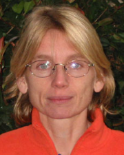
\includegraphics[width=1in]{content/monday/cortes-headshot.png}
%%     & {\bfseries Corinna Cortes} \newline Google Research, NY
%%   \end{tabular}
%% \end{center}

\daydateyear, 9:00--10:10am \vspace{1em}\\
\PlenaryLoc \\
\vspace{1em}\par
%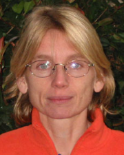
\includegraphics[height=100px]{content/monday/cortes-headshot.png}
\end{center}

\noindent
{\bfseries Abstract:} Police body-cameras have the potential to play an important
role in understanding and improving police-community relations.
In this talk I describe a series of studies conducted by our
large interdisciplinary team at Stanford that use speech and
natural language processing on body-camera recordings to model the interactions
between police officers and community members in traffic stops.
We use text and speech features to automatically measure linguistic aspects of the interaction,
from discourse factors like conversational structure to social factors like respect.
I describe the differences we find in the language directed toward black versus white community members,
and offer suggestions for how these findings can be used to help improve the fraught relations between
police officers and the communities they serve.

\vspace{3em}\par 

\vfill
\noindent

{\bfseries Biography:} Dan Jurafsky is Professor and Chair of Linguistics and Professor
  of Computer Science, at Stanford University.  His research has
  focused on the extraction of meaning, intention, and affect from
  text and speech, on the processing of Chinese, and on applying
  natural language processing to the cognitive and social sciences.
  Dan's deep interest in NLP education led him to co-write with Jim
  Martin the widely-used textbook "Speech and Language Processing”
  (whose 3rd edition is in (slow) progress) and co-teach with Chris Manning
  the first massive open online class on natural language processing.
  Dan was the recipient of the 2002 MacArthur Fellowship and is a
  2015 James Beard Award Nominee for his book, "The Language of Food:
  A Linguist Reads the Menu".

\newpage


%% Sessions  %%%%%%%%%%%%%%%%%%%%%%%%%%%%%%%%%%%%%%%%%%%%%%%%%%%%

%\clearpage
\setheaders{Session 1}{\daydateyear}
\begin{ThreeSessionOverview}{Session 1}{\daydateyear}
  {Semantics (Long Papers)}
  {Tagging, Chunking, Syntax and Parsing (Long + TACL Papers)}
  {Information Retrieval, Text Categorization, Topic Modeling (Long Papers)}
  \marginnote{\rotatebox{90}{10:40}}[2mm]
  \papertableentry{papers-455} & \papertableentry{papers-560} & \papertableentry{papers-533}
  \\
  \hline
  \marginnote{\rotatebox{90}{11:05}}[2mm]
  \papertableentry{papers-550} & \papertableentry{papers-136} & \papertableentry{papers-634}
  \\
  \hline
  \marginnote{\rotatebox{90}{11:30}}[2mm]
  \papertableentry{papers-670} & \papertableentry{papers-540} & \papertableentry{papers-353}
  \\
  \hline
  \marginnote{\rotatebox{90}{11:55}}[2mm]
  \papertableentry{papers-411} & \papertableentry{tacl-488} & \papertableentry{papers-073}
  \\
\end{ThreeSessionOverview}

\newpage
\section*{Parallel Session 1}
{\bfseries\large Session 1A: Semantics (Long Papers)}\\
\TrackALoc\hfill\sessionchair{Hoifung}{Poon}
\paperabstract{\day}{10:40--11:05}{}{}{papers-455}
\paperabstract{\day}{11:05--11:30}{}{}{papers-550}
\paperabstract{\day}{11:30--11:55}{}{}{papers-670}
\paperabstract{\day}{11:55--12:20}{}{}{papers-411}
\clearpage
{\bfseries\large Session 1B: Tagging, Chunking, Syntax and Parsing (Long + TACL Papers)}\\
\TrackBLoc\hfill\sessionchair{Noah A.}{Smith}
\paperabstract{\day}{10:40--11:05}{}{}{papers-560}
\paperabstract{\day}{11:05--11:30}{}{}{papers-136}
\paperabstract{\day}{11:30--11:55}{}{}{papers-540}
\paperabstract{\day}{11:55--12:20}{}{}{tacl-488}
\clearpage
{\bfseries\large Session 1C: Information Retrieval, Text Categorization, Topic Modeling (Long Papers)}\\
\TrackCLoc\hfill\sessionchair{Jordan}{Boyd-Graber}
\paperabstract{\day}{10:40--11:05}{}{}{papers-533}
\paperabstract{\day}{11:05--11:30}{}{}{papers-634}
\paperabstract{\day}{11:30--11:55}{}{}{papers-353}
\paperabstract{\day}{11:55--12:20}{}{}{papers-073}
\clearpage




%% Student lunch %%%%%%%%%%%%%%%%%%%%%%%%%%%%%%%%%%%%%%%%%%%%%%%%

%\clearpage
\section{Student Lunch}
\setheaders{}{\daydateyear}

\begin{center}

% \includegraphics[width=4in]{content/tuesday/aqua.jpg} \\

% {\tiny \copyright Public Domain}

\daydateyear, 12:30--2:00pm \vspace{1em}\\
\StudentLunchLoc \\
\end{center}

Join your fellow students for a free students-only lunch on \daydate
at 12:30 in the Plaza Ballroom C at the hotel.  Entrance tickets will
be in your conference badges. This is a chance to get to know others
who share similar interests and goals and who may become your lifelong
colleagues.


%% Sessions %%%%%%%%%%%%%%%%%%%%%%%%%%%%%%%%%%%%%%%%%%%%%%%%%%%%%

%\clearpage
\setheaders{Session 2}{\daydateyear}
\begin{ThreeSessionOverview}{Session 2}{\daydateyear}
  {Generation and Summarization (Long Papers)}
  {Language and Vision (Long Papers)}
  {NLP for Web, Social Media and Social Sciences (Long Papers)}
  \marginnote{\rotatebox{90}{2:00}}[2mm]
  \papertableentry{papers-055} & \papertableentry{papers-182} & \papertableentry{papers-039}
  \\
  \hline
  \marginnote{\rotatebox{90}{2:25}}[2mm]
  \papertableentry{papers-087} & \papertableentry{papers-356} & \papertableentry{papers-524}
  \\
  \hline
  \marginnote{\rotatebox{90}{2:50}}[2mm]
  \papertableentry{papers-278} & \papertableentry{papers-420} & \papertableentry{papers-575}
  \\
\end{ThreeSessionOverview}

\newpage
\section*{Parallel Session 2}
{\bfseries\large Session 2A: Generation and Summarization (Long Papers)}\\
\TrackALoc\hfill\sessionchair{Fei}{Liu}
\paperabstract{\day}{14:00--14:25}{}{}{papers-055}
\paperabstract{\day}{14:25--14:50}{}{}{papers-087}
\paperabstract{\day}{14:50--15:15}{}{}{papers-278}
\clearpage
{\bfseries\large Session 2B: Language and Vision (Long Papers)}\\
\TrackBLoc\hfill\sessionchair{Yejin}{Choi}
\paperabstract{\day}{14:00--14:25}{}{}{papers-182}
\paperabstract{\day}{14:25--14:50}{}{}{papers-356}
\paperabstract{\day}{14:50--15:15}{}{}{papers-420}
\clearpage
{\bfseries\large Session 2C: NLP for Web, Social Media and Social Sciences (Long Papers)}\\
\TrackCLoc\hfill\sessionchair{Tong}{Zhang}
\paperabstract{\day}{14:00--14:25}{}{}{papers-039}
\paperabstract{\day}{14:25--14:50}{}{}{papers-524}
\paperabstract{\day}{14:50--15:15}{}{}{papers-575}
\clearpage



%\clearpage
\setheaders{Session 3}{\daydateyear}
\begin{ThreeSessionOverview}{Session 3}{\daydateyear}
  {Generation and Summarization (Short Papers)}
  {Information Extraction and Question Answering (Short Papers)}
  {Machine Learning for NLP (Short Papers)}
  \marginnote{\rotatebox{90}{3:15}}[2mm]
  \papertableentry{papers-032} & \papertableentry{papers-664} & \papertableentry{papers-227}
  \\
  \hline
  \marginnote{\rotatebox{90}{3:30}}[2mm]
  \papertableentry{papers-477} & \papertableentry{papers-446} & \papertableentry{papers-631}
  \\
  \hline
  \marginnote{\rotatebox{90}{3:45}}[2mm]
  \papertableentry{papers-570} & \papertableentry{papers-674} & \papertableentry{papers-689}
  \\
\end{ThreeSessionOverview}

\newpage
\section*{Parallel Session 3}
{\bfseries\large Session 3A: Generation and Summarization (Short Papers)}\\
\TrackALoc\hfill\sessionchair{Fei}{Liu}
\paperabstract{\day}{15:15--15:30}{}{}{papers-032}
\paperabstract{\day}{15:30--15:45}{}{}{papers-477}
\paperabstract{\day}{15:45--16:00}{}{}{papers-570}
\clearpage
{\bfseries\large Session 3B: Information Extraction and Question Answering (Short Papers)}\\
\TrackBLoc\hfill\sessionchair{Yejin}{Choi}
\paperabstract{\day}{15:15--15:30}{}{}{papers-664}
\paperabstract{\day}{15:30--15:45}{}{}{papers-446}
\paperabstract{\day}{15:45--16:00}{}{}{papers-674}
\clearpage
{\bfseries\large Session 3C: Machine Learning for NLP (Short Papers)}\\
\TrackCLoc\hfill\sessionchair{Tong}{Zhang}
\paperabstract{\day}{15:15--15:30}{}{}{papers-227}
\paperabstract{\day}{15:30--15:45}{}{}{papers-631}
\paperabstract{\day}{15:45--16:00}{}{}{papers-689}
\clearpage




%\clearpage
%\section{One Minute Madness!}
%
%Prior to the poster session, TACL and long-paper poster presenters
%will be given one minute each to pitch their paper. The poster session
%will immediately follow these presentations along with a buffet
%dinner.
%\todo{Is this happening at EMNLP??}
%\sessionchair{Joel}{Tetreault}

%{\section{Poster session 1A}
{\setheaders{Poster session 1A}{\daydateyear}
{\large Time: \emph{6:00--7:30}\hfill Location: \PosterLoc}\\
\\
\posterabstract{papers-069}
\posterabstract{papers-123}
\posterabstract{papers-125}
\posterabstract{papers-167}
\posterabstract{papers-169}
\posterabstract{papers-205}
\posterabstract{papers-229}
\posterabstract{papers-232}
\posterabstract{papers-243}
\posterabstract{papers-263}
\posterabstract{papers-315}
\posterabstract{papers-367}
\posterabstract{papers-379}
\posterabstract{papers-421}
\posterabstract{papers-497}
\posterabstract{papers-521}
\posterabstract{papers-525}
\posterabstract{papers-529}
\posterabstract{papers-531}
\posterabstract{papers-541}
\posterabstract{papers-557}
\posterabstract{papers-589}
\posterabstract{papers-591}
\posterabstract{papers-595}
\posterabstract{papers-605}
\posterabstract{papers-617}
\posterabstract{papers-697}
\posterabstract{papers-699}
\posterabstract{papers-701}
\posterabstract{tacl-255}
\posterabstract{tacl-371}
\posterabstract{tacl-381}
\posterabstract{tacl-385}
\posterabstract{tacl-403}
\posterabstract{tacl-429}
\posterabstract{tacl-485}


%{\section{Poster session 1B}
{\setheaders{Poster session 1B}{\daydateyear}
{\large Time: \emph{7:30--9:00}\hfill Location: \PosterLoc}\\
\\
\posterabstract{papers-056}
\posterabstract{papers-090}
\posterabstract{papers-116}
\posterabstract{papers-150}
\posterabstract{papers-172}
\posterabstract{papers-178}
\posterabstract{papers-196}
\posterabstract{papers-218}
\posterabstract{papers-222}
\posterabstract{papers-226}
\posterabstract{papers-274}
\posterabstract{papers-296}
\posterabstract{papers-298}
\posterabstract{papers-306}
\posterabstract{papers-322}
\posterabstract{papers-336}
\posterabstract{papers-404}
\posterabstract{papers-428}
\posterabstract{papers-438}
\posterabstract{papers-448}
\posterabstract{papers-460}
\posterabstract{papers-552}
\posterabstract{papers-578}
\posterabstract{papers-586}
\posterabstract{papers-590}
\posterabstract{papers-648}
\posterabstract{tacl-452}
\posterabstract{tacl-472}


%{\section{SRW Poster Session}
{\setheaders{SRW Poster Session}{\daydateyear}
{\large Time: \emph{6:00--9:00}\hfill Location: \PosterLoc}\\
\\
\posterabstract{srw-004}
\posterabstract{srw-007}
\posterabstract{srw-011}
\posterabstract{srw-012}
\posterabstract{srw-013}
\posterabstract{srw-017}
\posterabstract{srw-023}
\posterabstract{srw-024}
\posterabstract{srw-028}
\posterabstract{srw-029}
\posterabstract{srw-030}
\posterabstract{srw-031}
\posterabstract{srw-040}
\posterabstract{srw-043}
\posterabstract{srw-047}
\posterabstract{srw-049}
\posterabstract{srw-051}
\posterabstract{srw-053}
\posterabstract{srw-056}
\posterabstract{srw-058}
\posterabstract{srw-059}
\posterabstract{srw-060}
\posterabstract{srw-062}




\setdaydateyear{Sunday}{September 10}{2017}
\chapter{Main Conference: \daydate}
\thispagestyle{emptyheader}
\setheaders{Main Conference}{\daydateyear}

%% Overview %%%%%%%%%%%%%%%%%%%%%%%%%%%%%%%%%%%%%%%%%%%%%%%%%%%%%
\section*{Overview}
\renewcommand{\arraystretch}{1.2}
\begin{SingleTrackSchedule}
  7:30 & -- & 9:00 &
  {\bfseries Registration and Breakfast} \hfill \emph{\RegistrationLoc}
  \\
  9:00 & -- & 10:40 &
  \begin{tabular}{|p{1.1in}|p{1.1in}|p{1.1in}|}
    \multicolumn{3}{l}{{\bfseries Session 4}}\\\hline
Dialogue and Spoken Language Processing (Long Papers) & Machine Learning for NLP (Long Papers) & Phonology, Morphology and Word Segmentation (Long Papers) \\
\emph{\TrackALoc} & \emph{\TrackBLoc} & \emph{\TrackCLoc} \\
  \hline\end{tabular} \\
  10:40 & -- & 11:15 &
  {\bfseries Break} \hfill \emph{\BreakLoc}
  \\
  11:15 & -- & 12:30 &
  \begin{tabular}{|p{1.1in}|p{1.1in}|p{1.1in}|}
    \multicolumn{3}{l}{{\bfseries Session 5}}\\\hline
Semantics (Short Papers) & Machine Translation (Short Papers) & Morphology, Syntax, Multilinguality, and Applications (Short Papers) \\
\emph{\TrackALoc} & \emph{\TrackBLoc} & \emph{\TrackCLoc} \\
  \hline\end{tabular} \\
  12:30 & -- & 2:00 &
  {\bfseries Lunch} \hfill \emph{\LunchLoc}
  \\
  2:00 & -- & 3:15 &
  \begin{tabular}{|p{1.1in}|p{1.1in}|p{1.1in}|}
    \multicolumn{3}{l}{{\bfseries Session 6}}\\\hline
Generation and Summarization (Long Papers) & Discourse and Coreference (Long Papers) & Information Extraction and Question Answering (Long Papers) \\
\emph{\TrackALoc} & \emph{\TrackBLoc} & \emph{\TrackCLoc} \\
  \hline\end{tabular} \\
  3:15 & -- & 3:45 &
  {\bfseries Break} \hfill \emph{\BreakLoc}
  \\
  3:45 & -- & 5:00 &
  \begin{tabular}{|p{1.1in}|p{1.1in}|p{1.1in}|}
    \multicolumn{3}{l}{{\bfseries Session 7}}\\\hline
Semantics (Long + TACL Papers) & Information Extraction and Question Answering (Long + TACL Papers) & Machine Translation (Long Papers) \\
\emph{\TrackALoc} & \emph{\TrackBLoc} & \emph{\TrackCLoc} \\
  \hline\end{tabular} \\
  5:00 & -- & 6:30 &
  {\bfseries Poster session 2A (Short papers)} \hfill \emph{\PosterLoc}
  \\
  5:00 & -- & 6:30 &
  {\bfseries Demo Session A} \hfill \emph{\DemoLoc}
  \\
  6:30 & -- & 8:00 &
  {\bfseries Poster session 2B (Short papers)} \hfill \emph{\PosterLoc}
  \\
  6:30 & -- & 8:00 &
  {\bfseries Demo Session B} \hfill \emph{\DemoLoc}
  \\
  8:00 & -- & 11:00 &
  {\bfseries Social Event} \hfill \emph{\SocialLoc}
  \\
\end{SingleTrackSchedule}
\newpage

%% Sessions %%%%%%%%%%%%%%%%%%%%%%%%%%%%%%%%%%%%%%%%%%%%%%%%%%%%%
\clearpage
\setheaders{Session 4}{\daydateyear}
\begin{ThreeSessionOverview}{Session 4}{\daydateyear}
  {Dialogue and Spoken Language Processing (Long Papers)}
  {Machine Learning for NLP (Long Papers)}
  {Phonology, Morphology and Word Segmentation (Long Papers)}
  \marginnote{\rotatebox{90}{9:00}}[2mm]
  \papertableentry{papers-490} & \papertableentry{papers-288} & \papertableentry{papers-688}
  \\
  \hline
  \marginnote{\rotatebox{90}{9:25}}[2mm]
  \papertableentry{papers-661} & \papertableentry{papers-407} & \papertableentry{papers-452}
  \\
  \hline
  \marginnote{\rotatebox{90}{9:50}}[2mm]
  \papertableentry{papers-082} & \papertableentry{papers-156} & \papertableentry{papers-671}
  \\
  \hline
  \marginnote{\rotatebox{90}{10:15}}[2mm]
  \papertableentry{papers-089} & \papertableentry{papers-176} & \papertableentry{papers-453}
  \\
\end{ThreeSessionOverview}

\newpage
\section*{Parallel Session 4}
{\bfseries\large Session 4A: Dialogue and Spoken Language Processing (Long Papers)}\\
\TrackALoc\hfill\sessionchair{Marilyn}{Walker}
\paperabstract{\day}{09:00--09:25}{}{}{papers-490}
\paperabstract{\day}{09:25--09:50}{}{}{papers-661}
\paperabstract{\day}{09:50--10:15}{}{}{papers-082}
\paperabstract{\day}{10:15--10:40}{}{}{papers-089}
\clearpage
{\bfseries\large Session 4B: Machine Learning for NLP (Long Papers)}\\
\TrackBLoc\hfill\sessionchair{Amarnag}{Subramanya}
\paperabstract{\day}{09:00--09:25}{}{}{papers-288}
\paperabstract{\day}{09:25--09:50}{}{}{papers-407}
\paperabstract{\day}{09:50--10:15}{}{}{papers-156}
\paperabstract{\day}{10:15--10:40}{}{}{papers-176}
\clearpage
{\bfseries\large Session 4C: Phonology, Morphology and Word Segmentation (Long Papers)}\\
\TrackCLoc\hfill\sessionchair{Hal}{Daum\IeC {\'e} III}
\paperabstract{\day}{09:00--09:25}{}{}{papers-688}
\paperabstract{\day}{09:25--09:50}{}{}{papers-452}
\paperabstract{\day}{09:50--10:15}{}{}{papers-671}
\paperabstract{\day}{10:15--10:40}{}{}{papers-453}
\clearpage



\clearpage
\setheaders{Session 5}{\daydateyear}
\begin{ThreeSessionOverview}{Session 5}{\daydateyear}
  {Semantics (Short Papers)}
  {Machine Translation (Short Papers)}
  {Morphology, Syntax, Multilinguality, and Applications (Short Papers)}
  \marginnote{\rotatebox{90}{11:15}}[2mm]
  \papertableentry{papers-281} & \papertableentry{papers-207} & \papertableentry{papers-647}
  \\
  \hline
  \marginnote{\rotatebox{90}{11:30}}[2mm]
  \papertableentry{papers-050} & \papertableentry{papers-262} & \papertableentry{papers-508}
  \\
  \hline
  \marginnote{\rotatebox{90}{11:45}}[2mm]
  \papertableentry{papers-558} & \papertableentry{papers-275} & \papertableentry{papers-513}
  \\
  \hline
  \marginnote{\rotatebox{90}{12:00}}[2mm]
  \papertableentry{papers-577} & \papertableentry{papers-255} & \papertableentry{papers-582}
  \\
  \hline
  \marginnote{\rotatebox{90}{12:15}}[2mm]
  \papertableentry{papers-607} & \papertableentry{papers-418} & \papertableentry{papers-350}
  \\
\end{ThreeSessionOverview}

\newpage
\section*{Parallel Session 5}
{\bfseries\large Session 5A: Semantics (Short Papers)}\\
\TrackALoc\hfill\sessionchair{Daniel}{Gildea}
\paperabstract{\day}{11:15--11:30}{}{}{papers-281}
\paperabstract{\day}{11:30--11:45}{}{}{papers-050}
\paperabstract{\day}{11:45--12:00}{}{}{papers-558}
\paperabstract{\day}{12:00--12:15}{}{}{papers-577}
\paperabstract{\day}{12:15--12:30}{}{}{papers-607}
\clearpage
{\bfseries\large Session 5B: Machine Translation (Short Papers)}\\
\TrackBLoc\hfill\sessionchair{David}{Chiang}
\paperabstract{\day}{11:15--11:30}{}{}{papers-207}
\paperabstract{\day}{11:30--11:45}{}{}{papers-262}
\paperabstract{\day}{11:45--12:00}{}{}{papers-275}
\paperabstract{\day}{12:00--12:15}{}{}{papers-255}
\paperabstract{\day}{12:15--12:30}{}{}{papers-418}
\clearpage
{\bfseries\large Session 5C: Morphology, Syntax, Multilinguality, and Applications (Short Papers)}\\
\TrackCLoc\hfill\sessionchair{William}{Lewis}
\paperabstract{\day}{11:15--11:30}{}{}{papers-647}
\paperabstract{\day}{11:30--11:45}{}{}{papers-508}
\paperabstract{\day}{11:45--12:00}{}{}{papers-513}
\paperabstract{\day}{12:00--12:15}{}{}{papers-582}
\paperabstract{\day}{12:15--12:30}{}{}{papers-350}
\clearpage



\clearpage
\setheaders{Session 6}{\daydateyear}
\begin{ThreeSessionOverview}{Session 6}{\daydateyear}
  {Generation and Summarization (Long Papers)}
  {Discourse and Coreference (Long Papers)}
  {Information Extraction and Question Answering (Long Papers)}
  \marginnote{\rotatebox{90}{2:00}}[2mm]
  \papertableentry{papers-565} & \papertableentry{papers-036} & \papertableentry{papers-476}
  \\
  \hline
  \marginnote{\rotatebox{90}{2:25}}[2mm]
  \papertableentry{papers-254} & \papertableentry{papers-673} & \papertableentry{papers-047}
  \\
  \hline
  \marginnote{\rotatebox{90}{2:50}}[2mm]
  \papertableentry{papers-567} & \papertableentry{papers-535} & \papertableentry{papers-317}
  \\
\end{ThreeSessionOverview}

\newpage
\section*{Parallel Session 6}
{\bfseries\large Session 6A: Generation and Summarization (Long Papers)}\\
\TrackALoc\hfill\sessionchair{Wei}{Xu}
\paperabstract{\day}{14:00--14:25}{}{}{papers-565}
\paperabstract{\day}{14:25--14:50}{}{}{papers-254}
\paperabstract{\day}{14:50--15:15}{}{}{papers-567}
\clearpage
{\bfseries\large Session 6B: Discourse and Coreference (Long Papers)}\\
\TrackBLoc\hfill\sessionchair{Ani}{Nenkova}
\paperabstract{\day}{14:00--14:25}{}{}{papers-036}
\paperabstract{\day}{14:25--14:50}{}{}{papers-673}
\paperabstract{\day}{14:50--15:15}{}{}{papers-535}
\clearpage
{\bfseries\large Session 6C: Information Extraction and Question Answering (Long Papers)}\\
\TrackCLoc\hfill\sessionchair{Lucy}{Vanderwende}
\paperabstract{\day}{14:00--14:25}{}{}{papers-476}
\paperabstract{\day}{14:25--14:50}{}{}{papers-047}
\paperabstract{\day}{14:50--15:15}{}{}{papers-317}
\clearpage



\clearpage
\setheaders{Session 7}{\daydateyear}
\begin{ThreeSessionOverview}{Session 7}{\daydateyear}
  {Semantics (Long + TACL Papers)}
  {Information Extraction and Question Answering (Long + TACL Papers)}
  {Machine Translation (Long Papers)}
  \marginnote{\rotatebox{90}{3:45}}[2mm]
  \papertableentry{papers-573} & \papertableentry{papers-369} & \papertableentry{papers-071}
  \\
  \hline
  \marginnote{\rotatebox{90}{4:10}}[2mm]
  \papertableentry{tacl-398} & \papertableentry{tacl-494} & \papertableentry{papers-293}
  \\
  \hline
  \marginnote{\rotatebox{90}{4:35}}[2mm]
  \papertableentry{tacl-457} & \papertableentry{tacl-412} & \papertableentry{papers-532}
  \\
\end{ThreeSessionOverview}

\newpage
\section*{Parallel Session 7}
{\bfseries\large Session 7A: Semantics (Long + TACL Papers)}\\
\TrackALoc\hfill\sessionchair{Xiaodong}{He}
\paperabstract{\day}{15:45--16:10}{}{}{papers-573}
\paperabstract{\day}{16:10--16:35}{}{}{tacl-398}
\paperabstract{\day}{16:35--17:00}{}{}{tacl-457}
\clearpage
{\bfseries\large Session 7B: Information Extraction and Question Answering (Long + TACL Papers)}\\
\TrackBLoc\hfill\sessionchair{Vincent}{Ng}
\paperabstract{\day}{15:45--16:10}{}{}{papers-369}
\paperabstract{\day}{16:10--16:35}{}{}{tacl-494}
\paperabstract{\day}{16:35--17:00}{}{}{tacl-412}
\clearpage
{\bfseries\large Session 7C: Machine Translation (Long Papers)}\\
\TrackCLoc\hfill\sessionchair{Hany}{Hassan}
\paperabstract{\day}{15:45--16:10}{}{}{papers-071}
\paperabstract{\day}{16:10--16:35}{}{}{papers-293}
\paperabstract{\day}{16:35--17:00}{}{}{papers-532}
\clearpage



{\section{Demo Session A}
{\setheaders{Demo Session A}{\daydateyear}
{\large Time: \emph{5:00--6:30}\hfill Location: \PosterLoc}\\
\\
\posterabstract{demos-011}
\posterabstract{demos-012}
\posterabstract{demos-016}
\posterabstract{demos-028}
\posterabstract{demos-029}
\posterabstract{demos-031}
\posterabstract{demos-034}
\posterabstract{demos-035}
\posterabstract{demos-038}
\posterabstract{demos-040}
\posterabstract{demos-046}
\posterabstract{demos-059}
\posterabstract{demos-061}


{\section{Demo Session B}
{\setheaders{Demo Session B}{\daydateyear}
{\large Time: \emph{6:30--8:00}\hfill Location: \PosterLoc}\\
\\
\posterabstract{demos-004}
\posterabstract{demos-005}
\posterabstract{demos-009}
\posterabstract{demos-014}
\posterabstract{demos-019}
\posterabstract{demos-021}
\posterabstract{demos-023}
\posterabstract{demos-037}
\posterabstract{demos-051}
\posterabstract{demos-055}
\posterabstract{demos-057}


\input{auto/papers/Tuesday-Poster-session-2A.tex}
\input{auto/papers/Tuesday-Poster-session-2B.tex}

%% Social event %%%%%%%%%%%%%%%%%%%%%%%%%%%%%%%%%%%%%%%%%%%%%%%%%

\clearpage
\section{Social Event}
\setheaders{}{\daydateyear}

\begin{center}

% \includegraphics[width=4in]{content/tuesday/aqua.jpg} \\

% {\tiny \copyright Public Domain}

\daydateyear, 20:00--23:00\vspace{1em}\\
\BanquetLoc\\
\end{center}

The  EMNLP 2017 social event will take place in the court yard just outside the venue, directly after the last session of Sunday. Some social events are designed to give attendees a chance to see a popular tourist attraction, but this year, the social event is pure fun and relaxation. All attendees are invited to grab free food at our food trucks, listen to great music, or just chill in the lounge areas. Of course the social event will include surprises, also, but - hey, they’re surprises. 



\setdaydateyear{Monday}{September 11}{2017}
\chapter{Main Conference: \daydate}
\thispagestyle{emptyheader}
\setheaders{Main Conference}{\daydateyear}

%% Overview %%%%%%%%%%%%%%%%%%%%%%%%%%%%%%%%%%%%%%%%%%%%%%%%%%%%%
\section*{Overview}
\renewcommand{\arraystretch}{1.2}
\begin{SingleTrackSchedule}
  07:30 & -- & 17:30 &
  {\bfseries Registration Day 3} \hfill \emph{\RegistrationLoc}
  \\
  08:00 & -- & 09:00 &
  {\bfseries Morning Coffee} \hfill \emph{\MorningLoc}
  \\
  09:00 & -- & 10:00 &
  {\bfseries Plenary Session. Invited Talk (Dan Jurafsky # )} \hfill \emph{\PlenaryLoc}
  \\
  10:00 & -- & 10:30 &
  {\bfseries Coffee Break} \hfill \emph{\CoffeeLoc}
  \\
  10:30 & -- & 12:10 &
  \begin{tabular}{|p{1.2in}|p{1.2in}|p{1.2in}|}
    \multicolumn{3}{l}{{\bfseries Session 7}}\\\hline
Machine Learning 3 # & Syntax 4 # & Dialogue # \\
\emph{\TrackALoc} & \emph{\TrackBLoc} & \emph{\TrackCLoc} \\
\hline
Poster Session. Machine Translation and Multilingual NLP 2 # & Poster Session. Information Extraction 2 # & Poster Session. NLP Applications # \\
\emph{\TrackDLoc} & \emph{\TrackELoc} & \emph{\TrackFLoc} \\
  \hline\end{tabular} \\
  12:10 & -- & 13:40 &
  {\bfseries Lunch} \hfill \emph{\LunchLoc}
  \\
  13:40 & -- & 15:25 &
  \begin{tabular}{|p{1.2in}|p{1.2in}|p{1.2in}|}
    \multicolumn{3}{l}{{\bfseries Session 8}}\\\hline
Machine Translation and Multilingual/Multimodal NLP (Short) # & Machine Learning (Short) # & NLP Applications (Short) # \\
\emph{\TrackALoc} & \emph{\TrackBLoc} & \emph{\TrackCLoc} \\
  \hline\end{tabular} \\
  15:25 & -- & 15:50 &
  {\bfseries Coffee Break} \hfill \emph{\CoffeeLoc}
  \\
  15:50 & -- & 17:25 &
  {\bfseries SESSION [('Monday', 'September 11', '2017')/15:50--17:25] Plenary Session. Best Paper # None None} \hfill \emph{\TODO LocationLoc}
  \\
  17:25 & -- & 17:45 &
  {\bfseries Closing Remarks (General Chair)} \hfill \emph{\ClosingLoc}
  \\
  17:25 & -- & 17:45 &
  {\bfseries SESSION [('Monday', 'September 11', '2017')/17:25--17:45] Plenary Session. Closing Remarks # None None} \hfill \emph{\TODO LocationLoc}
  \\
\end{SingleTrackSchedule}
\newpage

%% Invited Talk %%%%%%%%%%%%%%%%%%%%%%%%%%%%%%%%%%%%%%%%%%%%%%%%%
%\thispagestyle{myheadings}
\section{Invited Talk: Dan Jurafsky}
\index{Jurafsky, Dan}

\begin{center}
\begin{Large}
{\bfseries\Large ``Does This Vehicle Belong to You''? Processing the Language of Policing for Improving Police-Community Relations}\vspace{1em}\par
\end{Large}

%% \begin{center}
%%   \begin{tabular}{m{1in}b{1in}}
%%     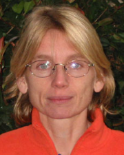
\includegraphics[width=1in]{content/monday/cortes-headshot.png}
%%     & {\bfseries Corinna Cortes} \newline Google Research, NY
%%   \end{tabular}
%% \end{center}

\daydateyear, 9:00--10:10am \vspace{1em}\\
\PlenaryLoc \\
\vspace{1em}\par
%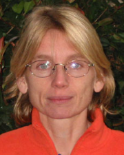
\includegraphics[height=100px]{content/monday/cortes-headshot.png}
\end{center}

\noindent
{\bfseries Abstract:} Police body-cameras have the potential to play an important
role in understanding and improving police-community relations.
In this talk I describe a series of studies conducted by our
large interdisciplinary team at Stanford that use speech and
natural language processing on body-camera recordings to model the interactions
between police officers and community members in traffic stops.
We use text and speech features to automatically measure linguistic aspects of the interaction,
from discourse factors like conversational structure to social factors like respect.
I describe the differences we find in the language directed toward black versus white community members,
and offer suggestions for how these findings can be used to help improve the fraught relations between
police officers and the communities they serve.

\vspace{3em}\par 

\vfill
\noindent

{\bfseries Biography:} Dan Jurafsky is Professor and Chair of Linguistics and Professor
  of Computer Science, at Stanford University.  His research has
  focused on the extraction of meaning, intention, and affect from
  text and speech, on the processing of Chinese, and on applying
  natural language processing to the cognitive and social sciences.
  Dan's deep interest in NLP education led him to co-write with Jim
  Martin the widely-used textbook "Speech and Language Processing”
  (whose 3rd edition is in (slow) progress) and co-teach with Chris Manning
  the first massive open online class on natural language processing.
  Dan was the recipient of the 2002 MacArthur Fellowship and is a
  2015 James Beard Award Nominee for his book, "The Language of Food:
  A Linguist Reads the Menu".

\newpage
\newpage

%% Sessions %%%%%%%%%%%%%%%%%%%%%%%%%%%%%%%%%%%%%%%%%%%%%%%%%%%%%
\clearpage
\setheaders{Session 7}{\daydateyear}
\begin{ThreeSessionOverview}{Session 7}{\daydateyear}
  {Machine Learning 3 #}
  {Syntax 4 #}
  {Dialogue #}
  \marginnote{\rotatebox{90}{10:30}}[2mm]
  \papertableentry{papers-1310} & \papertableentry{papers-264} & \papertableentry{papers-1270}
  \\
  \midrule
  \marginnote{\rotatebox{90}{10:55}}[2mm]
  \papertableentry{papers-349} & \papertableentry{papers-559} & \papertableentry{papers-1403}
  \\
  \midrule
  \marginnote{\rotatebox{90}{11:20}}[2mm]
  \papertableentry{papers-977} & \papertableentry{papers-1113} & \papertableentry{papers-1372}
  \\
  \midrule
  \marginnote{\rotatebox{90}{11:45}}[2mm]
  \papertableentry{papers-916} & \papertableentry{papers-1525} & \papertableentry{papers-1530}
  \\
\end{ThreeSessionOverview}

{\large {\bf Poster tracks}} \hfill 10:30--12:10 \\ \\ 
\vspace{1em}
{\bf Track D}: {\it Poster Session. Machine Translation and Multilingual NLP 2 #} \hfill \TrackDLoc
\\
\vspace{1em}
{\bf Track E}: {\it Poster Session. Information Extraction 2 #} \hfill \TrackELoc
\\
\vspace{1em}
{\bf Track F}: {\it Poster Session. NLP Applications #} \hfill \TrackFLoc
\\
\newpage
\section*{Parallel Session 7}
{\bfseries\large Session 7A: Machine Learning 3 #}\\
\TrackALoc\hfill Chair: \sessionchair{Barbara}{Plank}\\
\paperabstract{\day}{10:30--10:55}{}{}{papers-1310}
\paperabstract{\day}{10:55--11:20}{}{}{papers-349}
\paperabstract{\day}{11:20--11:45}{}{}{papers-977}
\paperabstract{\day}{11:45--12:10}{}{}{papers-916}
\clearpage
{\bfseries\large Session 7B: Syntax 4 #}\\
\TrackBLoc\hfill Chair: \sessionchair{Zeljko}{Agic}\\
\paperabstract{\day}{10:30--10:55}{}{}{papers-264}
\paperabstract{\day}{10:55--11:20}{}{}{papers-559}
\paperabstract{\day}{11:20--11:45}{}{}{papers-1113}
\paperabstract{\day}{11:45--12:10}{}{}{papers-1525}
\clearpage
{\bfseries\large Session 7C: Dialogue #}\\
\TrackCLoc\hfill Chair: \sessionchair{Amanda}{Stent}\\
\paperabstract{\day}{10:30--10:55}{}{}{papers-1270}
\paperabstract{\day}{10:55--11:20}{}{}{papers-1403}
\paperabstract{\day}{11:20--11:45}{}{}{papers-1372}
\paperabstract{\day}{11:45--12:10}{}{}{papers-1530}
\clearpage


{\bfseries\large Session 7D: Poster Session. Machine Translation and Multilingual NLP 2 #} \hfill 10:30--12:10 \\
\TrackDLoc\hfill Chair: \sessionchair{Marianna}{Apidianaki} \\
\\
\posterabstract{papers-1526}
\posterabstract{papers-194}
\posterabstract{papers-477}
\posterabstract{papers-1274}
\posterabstract{papers-1073}
\posterabstract{papers-1236}
\posterabstract{papers-1131}
\posterabstract{papers-1424}
\posterabstract{papers-1023}
\posterabstract{papers-817}
\posterabstract{papers-077}
\posterabstract{papers-1533}
\posterabstract{papers-637}

 \\
\clearpage \\
{\bfseries\large Session 7E: Poster Session. Information Extraction 2 #} \hfill 10:30--12:10 \\
\TrackBLoc\hfill Chair: \sessionchair{Isabelle}{Augenstein} \\
\\
\posterabstract{papers-119}
\posterabstract{papers-142}
\posterabstract{papers-529}
\posterabstract{papers-625}
\posterabstract{papers-1044}
\posterabstract{papers-1094}
\posterabstract{papers-1301}
\posterabstract{papers-634}
\posterabstract{papers-1324}
\posterabstract{papers-1408}
\posterabstract{papers-1005}
\posterabstract{papers-1356}
\posterabstract{papers-1295}

 \\
\clearpage \\
{\bfseries\large Session 7F: Poster Session. NLP Applications #} \hfill 10:30--12:10 \\
\TrackFLoc\hfill Chair: \sessionchair{Courtney}{Napoles} \\
\\
\posterabstract{papers-642}
\posterabstract{papers-049}
\posterabstract{papers-236}
\posterabstract{papers-282}
\posterabstract{papers-488}
\posterabstract{papers-674}
\posterabstract{papers-1184}
\posterabstract{papers-247}
\posterabstract{papers-747}
\posterabstract{papers-986}
\posterabstract{papers-1013}
\posterabstract{papers-457}
\posterabstract{papers-1254}

 \\
\clearpage \\

\clearpage
\setheaders{Session 8}{\daydateyear}
\begin{ThreeSessionOverview}{Session 8}{\daydateyear}
  {Multilingal/Multi-modal NLP and MT (Short) #}
  {Machine Learning (Short) #}
  {NLP Applications(?) #}
  \marginnote{\rotatebox{90}{13:40}}[2mm]
  \papertableentry{papers-1411} & \papertableentry{papers-1411} & \papertableentry{papers-1411}
  \\
  \midrule
  \marginnote{\rotatebox{90}{13:55}}[2mm]
  \papertableentry{papers-469} & \papertableentry{papers-469} & \papertableentry{papers-469}
  \\
  \midrule
  \marginnote{\rotatebox{90}{14:10}}[2mm]
  \papertableentry{papers-716} & \papertableentry{papers-716} & \papertableentry{papers-716}
  \\
  \midrule
  \marginnote{\rotatebox{90}{14:25}}[2mm]
  \papertableentry{papers-1511} & \papertableentry{papers-1511} & \papertableentry{papers-1511}
  \\
  \midrule
  \marginnote{\rotatebox{90}{14:40}}[2mm]
  \papertableentry{papers-644} & \papertableentry{papers-644} & \papertableentry{papers-644}
  \\
  \midrule
  \marginnote{\rotatebox{90}{14:55}}[2mm]
  \papertableentry{papers-538} & \papertableentry{papers-538} & \papertableentry{papers-538}
  \\
  \midrule
  \marginnote{\rotatebox{90}{15:10}}[2mm]
  \papertableentry{papers-1388} & \papertableentry{papers-1388} & \papertableentry{papers-1388}
  \\
\end{ThreeSessionOverview}

\newpage
\section*{Parallel Session 8}
{\bfseries\large Session 8A: Multilingal/Multi-modal NLP and MT (Short) #}\\
\TrackALoc\hfill\sessionchair{}{}
\paperabstract{\day}{13:40--13:55}{}{}{papers-1411}
\paperabstract{\day}{13:55--14:10}{}{}{papers-469}
\paperabstract{\day}{14:10--14:25}{}{}{papers-716}
\paperabstract{\day}{14:25--14:40}{}{}{papers-1511}
\paperabstract{\day}{14:40--14:55}{}{}{papers-644}
\paperabstract{\day}{14:55--15:10}{}{}{papers-538}
\paperabstract{\day}{15:10--15:25}{}{}{papers-1388}
\clearpage
{\bfseries\large Session 8B: Machine Learning (Short) #}\\
\TrackBLoc\hfill\sessionchair{}{}
\paperabstract{\day}{13:40--13:55}{}{}{papers-1411}
\paperabstract{\day}{13:55--14:10}{}{}{papers-469}
\paperabstract{\day}{14:10--14:25}{}{}{papers-716}
\paperabstract{\day}{14:25--14:40}{}{}{papers-1511}
\paperabstract{\day}{14:40--14:55}{}{}{papers-644}
\paperabstract{\day}{14:55--15:10}{}{}{papers-538}
\paperabstract{\day}{15:10--15:25}{}{}{papers-1388}
\clearpage
{\bfseries\large Session 8C: NLP Applications(?) #}\\
\TrackCLoc\hfill\sessionchair{}{}
\paperabstract{\day}{13:40--13:55}{}{}{papers-1411}
\paperabstract{\day}{13:55--14:10}{}{}{papers-469}
\paperabstract{\day}{14:10--14:25}{}{}{papers-716}
\paperabstract{\day}{14:25--14:40}{}{}{papers-1511}
\paperabstract{\day}{14:40--14:55}{}{}{papers-644}
\paperabstract{\day}{14:55--15:10}{}{}{papers-538}
\paperabstract{\day}{15:10--15:25}{}{}{papers-1388}
\clearpage



\section{Plenary Session. Best Papers.} \hfill 15:50--17:25 \\
\TrackALoc\hfill Chairs: \sessionchair{Rebecca}{Hwa}
, \sessionchair{Sebastian}{Riedel}
\\
\\
\posterabstract{papers-1470}
\posterabstract{papers-505}
\posterabstract{papers-633}
\posterabstract{papers-341}


\input{content/day3/honorable-mentions.tex}

%% Business meeting %%%%%%%%%%%%%%%%%%%%%%%%%%%%%%%%%%%%%%%%%%%%%
\clearpage
\section[SIGDAT Business Meeting]{SIGDAT Business Meeting}
%\thispagestyle{emptyheader}
\setheaders{SIGDAT Business Meeting \& Social Event}{\daydate}

\textbf{Date}: \daydateyear \\
\textbf{Time}: 13:00--13:45 \\
\textbf{Venue}: \BusinessMeetingLoc

Chair: \sessionchair{Noah}{Smith}

All attendees are encouraged to participate in the business
meeting. 
\newpage

%\input{auto/papers/Monday-Best-Paper-Plenary-Session.tex}


%% MISC %%%%%%%%%%%%%%%%%%%%%%%%%%%%%%%%%%%%%%%%%%%%%%%%%%%%%%%%%
% Anti-harassment policy
\chapter[Anti-harassment policy]{Anti-harassment policy}
\thispagestyle{emptyheader}
\setheaders{}{}
The open exchange of ideas, the freedom of thought and expression, and respectful scientific debate are central to the aims and goals of the ACL. These require a community and an environment that recognizes the inherent worth of every person and group, that fosters dignity, understanding, and mutual respect, and that embraces diversity. For these reasons, ACL is dedicated to providing a harassment-free experience for all the members, as well as participants at our events and in our programs.

Harassment and hostile behavior are unwelcome at any ACL conference, associated event, or in ACL-affiliated on-line discussions. This includes: speech or behavior that intimidates, creates discomfort, or interferes with a person's participation or opportunity for participation in a conference or an event. We aim for ACL-related activities to be an environment where harassment in any form does not happen, including but not limited to: harassment based on race, gender, religion, age, color, appearance, national origin, ancestry, disability, sexual orientation, or gender identity. Harassment includes degrading verbal comments, deliberate intimidation, stalking, harassing photography or recording, inappropriate physical contact, and unwelcome sexual attention. The policy is not intended to inhibit challenging scientific debate, but rather to promote it through ensuring that all are welcome to participate in shared spirit of scientific inquiry.

It is the responsibility of the community as a whole to promote an inclusive and positive environment for our scholarly activities. In addition, anyone who experiences harassment or hostile behavior may contact any current member of the ACL Executive Committee or contact Priscilla Rasmussen, who is usually available at the registration desk during ACL conferences. Members of the executive committee will be instructed to keep any such contact in strict confidence, and those who approach the committee will be consulted before any actions are taken.

Approved by ACL Executive Committee in 2016.

The policy is also available from ACL's main page.


\cleardoublepage
\addcontentsline{toc}{chapter}{Author Index}
\setheaders{Author Index}{Author Index}

\printindex

%% LOCAL GUIDE %%%%%%%%%%%%%%%%%%%%%%%%%%%%%%%%%%%%%%%%%%%%%%%%%%

\setheaders{Local Guide}{Local Guide}
%%%%%%%%%%%%%%%%%%%%%%%%%%%%%%%%%%%%%%%%%%%%%%%%%%%%%%%%%%%%%%%%%%%%%
% These are declarations of environments 
%%%%%%%%%%%%%%%%%%%%%%%%%%%%%%%%%%%%%%%%%%%%%%%%%%%%%%%%%%%%%%%%%%%%%

% the parameters are: title, description, address, url, opening hours
\newenvironment{funitem}[5]{
\noindent\textbf{#1}
\par \noindent\emph{#2}
\par \noindent{#4}
\par\noindent\begin{minipage}[b]{.37\textwidth}{#3}\end{minipage}\begin{minipage}[b]{.63\textwidth}{#5}\end{minipage}
\medskip
}

% the parameters are: title, description, address, url
\newenvironment{funitemshortaddr}[4]{
\noindent\textbf{#1}
\par \noindent\emph{#2}
\par \noindent{#4}
\par\noindent{#3}
\medskip
}

% fun item w/o address or opening hours
\newenvironment{funitemshort}[3]{
\noindent\textbf{#1}
\par \noindent\emph{#2}
\par \noindent{#3}
\medskip
}

% the parameters are: title, description, address, opening hours
\newenvironment{funitemwourl}[4]{
\noindent\textbf{#1}
\par \noindent\emph{#2}
\par\noindent\begin{minipage}[b]{.37\textwidth}{#3}\end{minipage}\begin{minipage}[b]{.63\textwidth}{#4}\end{minipage}
\medskip
}

% the parameters are: title, description, address, url
\newenvironment{shopitem}[4]{%
\noindent\textbf{#1.}\ \emph{#2.}\ #3\ #4%
}

% the parameters are: title, description, address, url
\newenvironment{eventitem}[4]{%
\noindent\textbf{#1.}\ #2.\ #3\ #4%
}

% the parameters are: title, description, address, url, distance, cost, opening hours
\newenvironment{fooditem}[7]{
\noindent
\begin{minipage}[t]{.5\textwidth}\textbf{#1} \end{minipage}\begin{minipage}[t]{.3\textwidth}\end{minipage}\hfill\begin{minipage}[t]{.2\textwidth}\textbf{#5}\ \ \ \ \ \textbf{#6} \end{minipage}
\par \noindent\emph{#2}
\par \noindent\url{#4}
\par\noindent\begin{minipage}[t]{.37\textwidth}{#3}\end{minipage}\begin{minipage}[t]{.63\textwidth}{#7}\end{minipage}
\medskip
}

% the parameters are: title, description, address, distance, cost, opening hours
\newenvironment{fooditemwourl}[6]{
\noindent
\begin{minipage}[t]{.5\textwidth}\textbf{#1} \end{minipage}\begin{minipage}[t]{.3\textwidth}\end{minipage}\hfill\begin{minipage}[t]{.2\textwidth}\textbf{#4}\ \ \ \ \ \textbf{#5}\end{minipage}
\par \noindent\emph{#2}
\par \noindent\begin{minipage}[t]{.37\textwidth}{#3}\end{minipage}\begin{minipage}[t]{.63\textwidth}{#6}\end{minipage}
\medskip
}

\newenvironment{ohours}[8]{%
{\begin{tabular}{l l l l} 
#1&#2&#5&#6 \\
#3&#4&#7&#8
\end{tabular}}
}

\newenvironment{addr}[2]{
{\begin{tabular}{l} 
#1\\
#2
\end{tabular}}
}

\newenvironment{shortaddr}[1]{
{\begin{tabular}{p{\textwidth}} 
#1
\end{tabular}}
}









%%%%%%%%%%%%%%%%%%%%%%%%%%%%%%%%%%%%%%%%%%%%%%%%%%%%%%%%%%%%%%%%%%%%%
% Start of Chapter
%%%%%%%%%%%%%%%%%%%%%%%%%%%%%%%%%%%%%%%%%%%%%%%%%%%%%%%%%%%%%%%%%%%%%


\chapter{Local Guide}


\emph{This guide was written by Maria Barrett, Joachim Bingel, Mareike Hartmann, Dirk Hovy.\\
\noindent For the most up-to-date version, please visit
  \url{http://www.emnlp2017.net}}
  
\index{Barrett, Maria}
\index{Bingel, Joachim}
\index{Hartmann, Mareike}
\index{Hovy, Dirk}



\section{General}
Welcome to Copenhagen!

To \textbf{get around} the city, best buy a multi-day pass or \textbf{rent bikes} at a local bike shop. There are also city bikes at many locations throughout the city. When biking, clearly indicate where you are going. Do not stop without indicating so (by raising a hand as if to greet someone). Do not swerve and change lanes. Any of these things will bring out the inner Viking in otherwise mild-mannered Danish cyclists.

\textbf{Public transport} is excellent and gets you everywhere. You certainly don't need a taxi between almost anywhere in the city and the airport. But note that there are three zones to get from the airport to central Copenhagen (and regular ticket controls!). Otherwise two zones will get you around central Copenhagen. Find connections between addresses in Denmark at \url{http://journeyplanner.dk}. If you stay longer and travel more than 10 times, you might want to get a \textbf{Rejsekort} (reloadable travel card valid throughout all of Denmark on all modes of transportation), which you can buy at vending machines placed at every metro station. Note that the card itself costs 80 DKK (non-refundable), and you’ll need to top it up before your first ride.
\par
For getting a sense of the \textbf{city’s geography}, it is helpful to realize that there are three major boroughs surrounding the Inner City in the West, North, and East, which are aptly called \textit{Vesterbro} (where the venue is located), \textit{Nørrebro}, and \textit{Østerbro}. Crammed between Vesterbro and Nørrebro lies \textit{Frederiksberg}. In the north, the Inner City is walled off by a stretch of artificial lakes, \textit{Søerne}, and in the south, on the other side of the canal, there’s the island of \textit{Amager}. 
\par
You can pay with \textbf{credit card} pretty much anywhere, although some places (usually smaller ones) require a Danish card.
\par
The \textbf{country code} is +45.


\section{Sightseeing}
Kødbyen is a lively place, and you can spend the entire conference within the walls of the old meatpacking district, trying new restaurants, listening to upcoming bands, and drinking hipster coffee with the locals. However, DGI Byen – the part of Kødbyen, in which Øksnehallen and Cph Conference are located – contains a number of other facilities. This includes indoor swimming and gym, that are free for participants. Check out \url{http://www.dgi-byen.com/} for more information. The following sightseeing suggestions all take you out of Kødbyen.
\par
\bigskip
\begin{funitem}
{Carlsberg Glyptotek}
{Nice collection of statues and paintings. The courtyard has a cafe where you can sit among palm trees. Free entrance on Tuesdays.}
{\begin{addr}
{Dantes Plads 7}
{1556 Copenhagen K}
\end{addr}}
{\url{http://www.glyptoteket.com}}
{\begin{ohours}
{Tue, Wed, Fri, Sat, Sun}
{11:00–18:00}
{Thu}
{11:00–22:00}
{}
{}
{}
{}
\end{ohours}}
\end{funitem}
\begin{funitemshortaddr}
{Christiania}
{Mostly known for weed and dead hippie dreams. Actually has nice jazz concerts and other events (often in ‘Operaen’, not to be confused with the big opera house). The old parts along the ramparts are full of nice, self-made houses. Nice vegetarian restaurant, Morgenstedet. }
{\begin{shortaddr}
{Main entrance is on Prinsessegade, but there are several other ways into the area.}
\end{shortaddr}}
{\url{http://www.visitcopenhagen.com/copenhagen/culture/alternative-christiania }}
\end{funitemshortaddr}
\begin{funitem}
{Danish Design Museum}
{Next to Kastellet in an old hospital. A series of several rooms arranged around a courtyard, each presenting one decade or artist of Danish design (lamps, chairs, etc.). Nice cafe, and a museum shop with many of the things you just saw.}
{\begin{addr}
{Bredgade 68}
{1260 Copenhagen K}
\end{addr}}
{\url{http://www.designmuseum.dk/en}}
{\begin{ohours}
{Tue, Fri, Thu, Sat, Sun}
{10:00–18:00}
{Wed}
{10:00–21:00}
{}
{}
{}
{}
\end{ohours}}
\end{funitem}
\begin{funitem}
{Den Sorte Diamant}
{The Royal Library. Modern addition to the old library. Great architecture. Changing exhibitions in the basement, a free exhibition of rare books and old manuscripts in a pop-art decorated room upstairs. Also features changing photography exhibitions.}
{\begin{addr}
{Søren Kierkegaards Pl. 1}
{1221 Copenhagen K}
\end{addr}}
{\url{http://www.kb.dk/en/}}
{\begin{ohours}
{Mon–Fri}
{08:00–21:00}
{Sat}
{09:00–19:00}
{}
{}
{}
{}
\end{ohours}}
\end{funitem}
\begin{funitem}
{Get a GoBoat}
{Get an electric-powered boat for up to eight people and set to sea (well, don’t actually set to sea: the canal). You can explore Copenhagen’s waterways on your own while enjoying some drinks and snacks that you bring yourself or pick up, e.g. at Papirøen.}
{\begin{addr}
{Islands Brygge 10}
{2300 Copenhagen S}
\end{addr}}
{\url{http://goboat.dk/en/}}
{\begin{ohours}
{}
{}
{}
{}
{}
{}
{}
{}
\end{ohours}}
\end{funitem}
\begin{funitemshort}
{Harbour bus}
{Cheapskate boat sightseeing. Pay a regular bus ticket or show your multi-day pass  and get a sea view of Copenhagen. Stops e.g. by Den Sorte Diamant, Nyhavn, The Opera House and Langelinje.}
{\url{https://www.google.dk/maps/place/Havnebussen/ }}
\end{funitemshort}
\noindent\textbf{Kastellet}
\par\noindent\emph{The old castle at the northern end of the city. Shaped like a star, and fun to walk on. Next to the Little Mermaid, which you can happily skip, but if you must, you can see it from here. Was built to defend the city, but captured before it was finished.}
\medskip

\begin{funitem}
{National Museum}
{One of the best Viking collections in the world.}
{\begin{addr}
{Ny Vestergade 10}
{1471 Copenhagen K}
\end{addr}}
{\url{http://en.natmus.dk/museums/the-national-museum-of-denmark/}}
{\begin{ohours}
{Tue–Sun}
{10:00–17:00}
{}
{}
{}
{}
{}
{}
\end{ohours}}
\end{funitem}
\begin{funitem}
{Rundetårn}
{Round tower with a spiraling pathway inside, built so that the king could ride up on a horse to the observatory. Nice view over the city, and you can run down the spiral and shout “wheeee!” }
{\begin{addr}
{Købmagergade 52A}
{1150 Copenhagen K}
\end{addr}}
{\url{http://www.rundetaarn.dk/en/}}
{\begin{ohours}
{All days}
{10:00–20:00}
{}
{}
{}
{}
{}
{}
\end{ohours}}
\end{funitem}
\begin{funitem}
{Torvehallerne}
{Two modern market halls, filled with food vendors and food-related items. Some overpriced stuff, but also a lot of specialized shops with things that are otherwise hard to find. The smørrebrød shop is becoming a new in-spot.}
{\begin{addr}
{Frederiksborggade 21}
{1360 Copenhagen K}
\end{addr}}
{\url{http://torvehallernekbh.dk}}
{\begin{ohours}
{Mon–Wed}
{10:00–19:00}
{Thu–Fri}
{10:00–20:00}
{Sat}
{10:00–18:00}
{Sun}
{11:00–17:00}
\end{ohours}}
\end{funitem}
\begin{funitemwourl}
{The Little Mermaid}
{Yeah… Don’t be too disappointed.}
{\begin{addr}
{Langelinie}
{2100 Copenhagen Ø}
\end{addr}}
{}
{\begin{ohours}
{}
{}
{}
{}
{}
{}
{}
{}
\end{ohours}}
\end{funitemwourl}
\begin{funitem}
{Statens Museum for Kunst}
{Decent art museum. Has a bar on the first Friday of the month.}
{\begin{addr}
{Sølvgade 48-50}
{1307 Copenhagen K}
\end{addr}}
{\url{http://www.smk.dk/en/}}
{\begin{ohours}
{Tue–Sun}
{11:00–17:00}
{Wed}
{11:00–20:00}
{}
{}
{}
{}
\end{ohours}}
\end{funitem}
\begin{funitemshort}
{Ørestad}
{If you like new architecture, take the metro and visit Ørestad. It is a new area of Copenhagen with award-winning houses. There is a mall directly in front of Ørestad station (Field’s), or take the metro out to Vestamager station and walk up the 8tallet house.}
{\url{http://www.visitcopenhagen.com/copenhagen/architecture/architectural-orestad}}
\end{funitemshort}
\begin{funitemshort}
{Jægersborggade}
{This street in Nørrebro is a hipster’s paradise. Very close to Assistens Kirkegård, it is home to a number of cafés/bars, galleries, craft and (second-hand) clothing shops, as well as combinations thereof (Sneakers\&Coffee, Beer\&Vinyl, \dots). Great for finding gifts to take home. }
{\url{http://jaegersborggade.com/wpAB/en/shops/}}
\end{funitemshort}

\section{Shops}

\begin{shopitem}
{B\&W Hallerne}%title
{Second hand furniture in a giant, factory hall, by the water, in industrial Copenhagen. Only open every other weekend. Bring cash}%description
{Refshalevej 171, 1432 Copenhagen.}%adress
{\url{https://www.facebook.com/BW-LOPPEMARKED-171235476283625/}}%url
\end{shopitem}

\begin{shopitem}
{Faraos Cigarer}%title
{Cartoon shop – or three, actually, but all next-door – close to Rundetårn}%description
{Skindergade 27, 1159 Copenhagen K.}%adress
{\url{https://www.faraos.dk}}%url
\end{shopitem}

\begin{shopitem}
{Sort kaffe \& Vinyl}%title
{Hipster record shop with good coffee}%description
{Skydebanegade 4
1709 Copenhagen V.}%adress
{\url{https://www.facebook.com/sortkaffeogvinyl/}}%url
\end{shopitem}

\begin{shopitem}
{København K}%title
{Second-hand clothing in a street packed with fashion stores}%description
{Studiestræde 30, 1455 Copenhagen K.}%adress
{\url{http://koebenhavnk.com}}%url
\end{shopitem}

\section*{Dance and Music Venues}
\begin{shopitem}
{Global CPH}%title
{World music}%description
{Nørre Allé 7, 2200 Copenhagen N.}%adress
{\url{http://globalcph.dk/english/}}%url
\end{shopitem}

\begin{shopitem}
{Danshallerne}%title
{Dance and theatre}%description
{Bohrsgade 19, 1799 Copenhagen V.}%adress
{\url{http://www.dansehallerne.dk/en/}}%url
\end{shopitem}

\begin{shopitem}
{La Fontaine}%title
{Intimate, 100-capacity veteran of the Scandinavian jazz scene staging nightly jam sessions}%description
{Kompagnistræde 11, 1208 Copenhagen K.}%adress
{\url{http://lafontaine.dk}}%url
\end{shopitem}

\begin{shopitem}
{Montmartre}%title
{Classic jazz joint in central Copenhagen}%description
{Store Regnegade 19A, 1110 Copenhagen K.}%adress
{\url{http://www.jazzhusmontmartre.dk}}%url
\end{shopitem}

\begin{shopitem}
{Mojo}%title
{Blues, jazz \& folk from Scandinavian \& international artists in a compact club open until 5am}%description
{Løngangstræde 21C, 1468 Copenhagen K.}%adress
{\url{https://mojo.dk}}%url
\end{shopitem}

\begin{shopitem}
{Pumpehuset}%title
{Rock, pop, hip hop, world music -- lots of different music styles, but generally nice, national and international bookings}%description
{Studiestræde 52, 1554 Copenhagen V.}%adress
{\url{http://pumpehuset.dk/}}%url
\end{shopitem}

\begin{shopitem}
{Royal Theatre}%title
{See ballet at the old stage, a play in the new theatre house by the sea or opera in the Opera House}%description
{}%adress
{\url{https://kglteater.dk/en/}}%url
\end{shopitem}

\begin{shopitem}
{Vega}%title
{Rock and pop scene not too far from the venue}%description
{Enghavevej 40, 1674 Copenhagen V.}%adress
{\url{http://vega.dk}}%url
\end{shopitem}



\section{Events}
Moreover, if your conference schedule permits, here’s a list of events happening in Copenhagen and the wider region, during EMNLP:
\par
\bigskip


\begin{eventitem}
{Cirque du Soleil}%title
{Malmö Arena, September 6--10}%description
{Hyllie Stationstorg 2, 215 32 Malmö, Sweden.}%adress
{\url{https://www.cirquedusoleil.com/sweden/malmo/shows}}%url
\end{eventitem}


\begin{eventitem}
{Copenhagen World Music}%title
{Runs September 6--10 at different venues in Copenhagen}%description
{}%adress
{\url{http://cphworld.dk}}%url
\end{eventitem}

\begin{eventitem}
{Luisi leads Danish composer Carl Nielsen’s 5th Symphony in Koncerthuset}%title
{September 7}%description
{Koncerthuset, Emil Holms Kanal 20, 2300 Copenhagen S.}%adress
{\url{http://drkoncerthuset.dk/}}%url
\end{eventitem}

\section{Day-Trips}

\begin{funitem}
{Arken}
{Modern art museum south of the city, in an unassuming suburb. Nice changing exhibitions and a modern collection. }
{\begin{addr}
{Skovvej 100}
{2635 Ishøj}
\end{addr}}
{\url{http://uk.arken.dk}}
{\begin{ohours}
{}
{}
{}
{}
{}
{}
{}
{}
\end{ohours}}
\end{funitem}
\begin{funitem}
{Louisiana}
{Modern art museum on the coast north of the city. The buildings are integrated into a park overlooking the cliffs towards Sweden. Great exhibits and a world-renowned collection. Sneak in picnic stuff and eat on the lawns.}
{\begin{addr}
{Gl Strandvej 13}
{3050 Humlebæk}
\end{addr}}
{\url{https://en.louisiana.dk}}
{\begin{ohours}
{}
{}
{}
{}
{}
{}
{}
{}
\end{ohours}}
\end{funitem}
\begin{funitem}
{Roskilde Viking Ship Museum}
{30 min by train from the main station, in a lovely small town lies this museum, which contains five well-preserved Viking ships that were sunk there to form a barrier. See the 1:1 viking ship reconstructions and try to sail one.}
{\begin{addr}
{Vindeboder 12}
{4000 Roskilde}
\end{addr}}
{\url{http://www.vikingeskibsmuseet.dk/en/}}
{\begin{ohours}
{}
{}
{}
{}
{}
{}
{}
{}
\end{ohours}}
\end{funitem}



\section{Other Things to Do}
If you’re less into classical sightseeing but want to live a day as a Copenhagener would (big claim, we know\dots), the following suggestions might be interesting. Obviously, the best way to get around is by bike.

\subsection{Dance the Night Away}
If you’re into electronic music, you’ll probably enjoy Copenhagen’s old Meat Packing District (\textit{Kødbyen}), where all the following bars are located. \textit{Jolene} and \textit{Bakken} are small and sweaty, and true to their origin and location. They look a bit run-down (the area used to be all slaughterhouses and meat auction halls). There’s also \textit{KB18} with more deep house/techno, but don’t go there before 1 am. \textit{Mesteren \& Lærlingen} plays hip hop/soul/reggae.

\subsection{Parks}
Copenhagen has a number of very nice parks that invite you to hang out or do sports. The biggest, \textit{Fælledparken}, is right next to the Department of Computer Science and has a little lake, otherwise it’s a big green meadow with lots of runners and football players. A hidden gem with a super beautiful (albeit artificially created) lake, or rather trench, is \textit{Østre Anlæg}, right behind the National Art Gallery. You can have a barbeque there if you bring your own coal, stationary grills are provided. \textit{Assistens Kirkegård} in Nørrebro is a very beautiful graveyard. People from other places might find this strange, but it’s a favourite pastime among Copenhageners to hang out here. \textit{Nørrebroparken} is wonderful in springtime, go there to join young Copenhageners for a beer or a frisbee game (disclaimer: don’t literally try to join them, they are Danes. They will panic). Just outside of Copenhagen near Gentofte station, is \textit{Bernstorff’s Park} which – aside from usual park stuff and a castle – holds Pometet which is a very broad range of Danish fruit trees as well as a smaller selection of exotic fruit trees. Originally for the royal family, but nowadays free for visitors to sample. During weekends in spring, summer and early autumn you can have afternoon tea in Queen Louise’ teahouse or in the her rose garden. 



\section{Eating \& Drinking}
Unless you come from Norway, everything will be more expensive than in your home country. It’s best not to convert the prices and just take them as-is. A coffee/latte costs 20--50 DKK, a beer almost everywhere 50 DKK. A main course in a restaurant is typically 150–250 DKK.
\par
The following sections list a selection of restaurants along with the price range and their distance from the conference venue.
\par
\medskip
\noindent Price range indicator: 

\begin{tabular}{l l} 
\textbf{\$} &Main course $<$ 150 DKK\\
\textbf{\$\$}&Main course 150–250 DKK\\
\textbf{\$\$\$} &Main course $>$ 250 DKK
\end{tabular}



\section{Restaurants Close to the Conference Venue}
The following restaurants are in very close proximity to the conference venue, most of them in \emph{Kødbyen}, the old meat packing district, which is now a center of Copenhagen nightlife and home to numerous restaurants offering foods from around the globe. The following are all great picks, but there are plenty more for you to discover.
\par
\bigskip
\begin{fooditem}
{Fiskebaren}
{Allegedly one of the 10 best fish restaurants in Europe. Very nice dishes, but expensive. Go for the starters and medium dishes and share. Make sure to check out the column-shaped aquarium.}
{\begin{addr}
{Flæsketorvet 100}
{1711 Copenhagen V}
\end{addr}}
{http://fiskebaren.dk}
{0.4 km}
{\$\$\$}
{\begin{ohours}
{Mon–Thu}
{17:30–00:00}
{Fri}
{17:30–02:00}
{Sat}
{11:30–02:00}
{Sun}
{11:30–00:00}
\end{ohours}}
\end{fooditem}
\begin{fooditem}
{Fleisch}
{Restaurant in Kødbyen with its own butcher counter. Have some meat-based open-face sandwiches there, or grab a few of their beer sausages to go and enjoy them outside.}
{\begin{addr}
{Slagterboderne 7}
{1716 Copenhagen V}
\end{addr}}
{http://www.fleisch.dk}
{0.3 km}
{\$\$}
{\begin{ohours}
{Tue--Thu}
{11:30--00:00}
{Fri--Sat}
{11:30--01:00}
{Sun}
{11:30--00:00}
{}
{}
\end{ohours}}
\end{fooditem}


\begin{fooditemwourl}
{Bio Mio Organic Bistro}
{Organic hearty bistro. Vegan and vegetarian options.}
{\begin{addr}
{Halmtorvet 19}
{1700 Copenhagen V}
\end{addr}}
{0.2 km}
{\$\$}
{\begin{tabular}{l l} 
Mon--Wed & 12:00--16:00 \& 17:00--22:00\\
Thu & 12:00--16:00 \& 17:00--22:30\\
Fri--Sat & 12:00--16:00 \& 17:30--22:30\\
Sun & 12:00--16:00 \& 17:00--21:00
\end{tabular}}
\end{fooditemwourl}



\begin{fooditem}
{Hija de Sanchez}
{Ex-Noma chef decided to leave the big business and make everyday tacos. Get 3 for 100DKK.}
{\begin{addr}
{Slagterboderne 8}
{1716 Copenhagen V}
\end{addr}}
{http://www.hijadesanchez.dk}
{0.3 km}
{\$}
{\begin{ohours}
{Mon–Fri}
{17:30–00:00}
{Sun}
{17:30–22:00}
{}
{}
{}
{}
\end{ohours}}
\end{fooditem}
\begin{fooditemwourl}
{Isted Grill}
{Not a restaurant, but a hole-in-the-wall late-night snack food place. Get the flæskesteg sandwich (grilled pork roast with pickles and red cabbage) after a night of drinking. Cheap and tasty.}
{\begin{addr}
{Istedgade 92}
{1650 Copenhagen V}
\end{addr}}
{0.7 km}
{\$}
{\begin{ohours}
{Sun–Thu}
{12:00–00:00}
{Fri–Sat}
{12:00–02.00}
{}
{}
{}
{}
\end{ohours}}
\end{fooditemwourl}
\begin{fooditem}
{Madklubben}
{Several locations, closest on Vesterbrogade. Nice “home-made” food, reasonable prices. Very good for groups (with a reservation). Vegetarian options. }
{\begin{addr}
{Vesterbrogade 62}
{1620 Copenhagen V}
\end{addr}}
{http://madklubben.dk/en/ }
{0.7 km}
{\$}
{\begin{ohours}
{Mon–Thu}
{17:30–00:00}
{Fri–Sat}
{17:00–00:00}
{}
{}
{}
{}
\end{ohours}}
\end{fooditem}
\begin{fooditem}
{Magasasa Dim Sum \& Cocktails}
{The name says it all. Raw interior. Reasonably priced. }
{\begin{addr}
{Flæsketorvet 54--56}
{1711 Copenhagen V}
\end{addr}}
{http://magasasa.dk/dim-sum-cocktails/?lang=en}
{0.5 km}
{\$}
{\begin{ohours}
{Mon–Thu}
{11:00–23:00}
{Fri–Sat}
{11:00–00:00}
{}
{}
{}
{}
\end{ohours}}
\end{fooditem}
\begin{fooditem}
{Mother}
{Great pizza!}
{\begin{addr}
{Høkerboderne 9}
{1712 Copenhagen V}
\end{addr}}
{http://mother.dk}
{0.4 km}
{\$}
{\begin{ohours}
{All days}
{11:00–01:00}
{}
{}
{}
{}
{}
{}
\end{ohours}}
\end{fooditem}
\begin{fooditem}
{Nose2Tail}
{As cozy as a former slaughterhouse basement can get (the one in the Kødbyen basement is the best of their locations). Serves daily changing meat, fish, and innard dishes. Freshly made cracklings (Danish delicacy made from pork skin), served with bacon mayonnaise – because fat! Chase with a Fernet Branca. Very good beer and friendly staff with awesome leather aprons.}
{\begin{addr}
{Kødboderne 9}
{1711 Copenhagen}
\end{addr}}
{http://nose2tail.dk/}
{0.6 km}
{\$\$}
{\begin{ohours}
{Tue–Thu}
{18:00–00:00}
{Fri–Sat}
{18:00–01:00}
{}
{}
{}
{}
\end{ohours}}
\end{fooditem}
\begin{fooditem}
{PatePate}
{Small plates, international cuisine. Great for sharing. Medium price range. Also nice to start your evening in Kødbyen. Vegetarian options. }
{\begin{addr}
{Slagterboderne 1}
{1716 Copenhagen V}
\end{addr}}
{http://www.patepate.dk/}
{0.2 km}
{\$\$}
{\begin{ohours}
{Mon–Wed}
{09:00–00:00}
{Thu}
{09:00–01:00}
{Fri}
{09:00–01:00}
{Sat}
{11:30–01:00}
\end{ohours}}
\end{fooditem}
\begin{fooditem}
{Restaurant Cofoco}
{Part of the Cooking for Copenhagen group. Small delicious plates. Slightly upscale, but reasonable.}
{\begin{addr}
{Abel Cathrines Gade 7}
{1654 Copenhagen V}
\end{addr}}
{http://cofoco.dk/en/}
{0.3 km}
{\$\$}
{\begin{ohours}
{Mon–Sat}
{18:00–00:00}
{}
{}
{}
{}
{}
{}
\end{ohours}}
\end{fooditem}
\begin{fooditem}
{Tommi’s Burger Joint}
{Tasty minimalistic burgers! Part of a small international chain originating from Iceland.}
{\begin{addr}
{Høkerboderne 21-23}
{1712 København V}
\end{addr}}
{https://www.burgerjoint.dk/}
{0.4 km}
{\$}
{\begin{ohours}
{Thu–Sun}
{11:00–22:00}
{Mon–Wed}
{11:00–21:00}
{}
{}
{}
{}
\end{ohours}}
\end{fooditem}
\begin{fooditem}
{WEDOFOOD}
{Homemade salads. Vegetarian options.}
{\begin{addr}
{Halmtorvet 21}
{1700 Copenhagen V}
\end{addr}}
{http://wedofood.dk}
{0.2 km}
{\$}
{\begin{ohours}
{Mon-Sat}
{10:00–21:00}
{Sun}
{10:00–20:00}
{}
{}
{}
{}
\end{ohours}}
\end{fooditem}
\begin{fooditem}
{Warpigs}
{One word: pork. Great craft beer.}
{\begin{addr}
{Flæsketorvet 25}
{1711 Copenhagen V}
\end{addr}}
{http://warpigs.dk}
{0.3 km}
{\$\$}
{\begin{ohours}
{Mon–Thu}
{11:30–00:00}
{Fri–Sat}
{11:00–02:00}
{}
{}
{}
{}
\end{ohours}}
\end{fooditem}






\section{Culinary Highlights in the City}

\begin{fooditem}
{Bror}
{High-end dining, comes with reasonably priced wine pairings. More expensive, but worth it.}
{\begin{addr}
{Sankt Peders Stræde 24A}
{1453 Copenhagen K}
\end{addr}}
{http://www.restaurantbror.dk }
{1.3 km}
{\$\$\$}
{\begin{ohours}
{Wed–Sun}
{17:30–00:00}
{}
{}
{}
{}
{}
{}
\end{ohours}}
\end{fooditem}
\begin{fooditem}
{Geist}
{Super-minimalist nordic cooking. The menu describes exactly what you get (“Carrots, braised in orange juice, with ginger”), but whatever it is, it’s cooked to perfection! You order several small plates, each reasonably priced, but it adds up. You can watch the busy, but eerily quiet kitchen, lit only by candles. Fancy cocktail bar, too, albeit a bit short on classics.}
{\begin{addr}
{Kongens Nytorv 8}
{1050 Copenhagen K}
\end{addr}}
{http://restaurantgeist.dk}
{2.3 km}
{\$\$}
{\begin{ohours}
{All days}
{12:00–15:00 and 17:30–01:00}
{}
{}
{}
{}
{}
{}
\end{ohours}}
\end{fooditem}
\begin{fooditem}
{Gran Torino}
{Part of the Madklubben group. Set meals (from 200 DKK) includes pasta, pizza and extra nice Tiramisu.}
{\begin{addr}
{Sortedam Dossering 5}
{2200 Copenhagen N}
\end{addr}}
{http://madklubben.dk/gran-torino/}
{2.3 km}
{\$}
{\begin{ohours}
{Mon–Fri}
{17:30–00:00}
{Sun}
{17:30–22:00}
{}
{}
{}
{}
\end{ohours}}
\end{fooditem}
\begin{fooditem}
{Höst}
{Get a fixed price menu with lots of interesting culinary and visual effects (clams on burning juniper bushes). Pricey, but worth the money. Throw in an extra few hundred for the wine pairing, and you won't be disappointed.}
{\begin{addr}
{Nørre Farimagsgade 41}
{1364 Copenhagen K}
\end{addr}}
{http://hostvakst.dk/host/restaurant/?lang=en}
{1.6 km}
{\$\$\$}
{\begin{ohours}
{All days}
{17:30–00:00}
{}
{}
{}
{}
{}
{}
\end{ohours}}
\end{fooditem}
\begin{fooditemwourl}
{Morgenstedet}
{Vegetarian Restaurant in the heart of Christiania. Has an improvised canteen feel to it, but very tasty food.}
{\begin{addr}
{Fabriksområdet 134}
{1440 Copenhagen K}
\end{addr}}
{3.3 km}
{\$}
{\begin{ohours}
{Tue–Sun}
{12:00–21:00}
{}
{}
{}
{}
{}
{}
\end{ohours}}
\end{fooditemwourl}
\begin{fooditem}
{Papirøen}
{A collection of street food vendors in one old factory building, ranging from duck-fat fries to Asian noodle salads. And plenty of drinks. If the weather is nice, you can sit in deck chairs and watch the boats on the canal. Cheap to mid-range depending on the vendor.}
{\begin{addr}
{Trangravsvej 14, hal 7/8}
{1436 Copenhagen K}
\end{addr}}
{http://copenhagenstreetfood.dk/en/}
{3.3 km}
{\$-\$\$}
{\begin{ohours}
{Mon–Thu}
{12:00–21:00}
{Fri–Sun}
{12:00–21:00}
{}
{}
{}
{}
\end{ohours}}
\end{fooditem}
\begin{fooditem}
{Ramen to Biiru}
{Japanese ramen meets Danish craft beer.}
{\begin{addr}
{Enghavevej 58}
{1674 Copenhagen V}
\end{addr}}
{http://ramentobiiru.dk/vesterbro/}
{1.4 km}
{\$}
{\begin{ohours}
{Mon--Thu}
{12:00–22:00}
{​​Fri-Sat}
{12:00–23:00}
{​Sun}
{12:00–21:00}
{}
{}
\end{ohours}}
\end{fooditem}
\begin{fooditem}
{SimpleRAW}
{Rawfood. Vegan and vegetarian.}
{\begin{addr}
{Gråbrødre Torv 9}
{1154 Copenhagen K}
\end{addr}}
{https://www.simpleraw.dk}
{1.7 km}
{\$}
{\begin{ohours}
{Mon-Sat}
{10:00–22:00}
{Sun}
{10:00–20:00}
{}
{}
{}
{}
\end{ohours}}
\end{fooditem}









\section{Cafés and Bars}

\begin{fooditem}
{Bang og Jensen}
{At the far end of Istedgade, both a cafe and a bar, and extremely hyggelig.}
{\begin{addr}
{Istedgade 130}
{1650 Copenhagen V}
\end{addr}}
{http://www.bangogjensen.dk}
{0.9 km}
{}
{\begin{ohours}
{Mon-Fri}
{07:30-02:00}
{Sat}
{10:00-02:00}
{Sun}
{10:00-00:00}
{}
{}
\end{ohours}}
\end{fooditem}
\begin{fooditem}
{Bastard}
{Board game café.}
{\begin{addr}
{Rådhusstræde 13}
{1466 Copenhagen K}
\end{addr}}
{http://bastardcafe.dk }
{1.3 km}
{}
{\begin{ohours}
{Mon–Thu, Sun}
{12:00–00:00}
{Fri–Sat}
{12:00–02:00}
{}
{}
{}
{}
\end{ohours}}
\end{fooditem}
\begin{fooditem}
{Kaffe}
{On Istedgade, at the intersection with Skydebanegade, and easy to miss. Full of wooden trinkets and good coffee. Very small!}
{\begin{addr}
{Istedgade 90}
{1650 Copenhagen V}
\end{addr}}
{http://kaffeistedgade.dk}
{0.7 km}
{}
{\begin{ohours}
{Mon–Fri}
{08:00–22:00}
{Sat–Sun}
{09:00–22:00}
{}
{}
{}
{}
\end{ohours}}
\end{fooditem}
\begin{fooditem}
{Library Bar}
{Next to the train station, the bar of the Plaza Hotel. Plush leather sofas, dark wood panels, and on some nights: live piano and songs. Mixed crowd, go in a suit or with hiking clothes.}
{\begin{addr}
{Bernstorffsgade 4}
{1577 Copenhagen V}
\end{addr}}
{https://ligula.se/en/the-library-bar/}
{0.6 km}
{}
{\begin{ohours}
{Mon–Thu}
{16:00–00:00}
{Fri–Sat}
{16:00–01:00}
{}
{}
{}
{}
\end{ohours}}
\end{fooditem}
\begin{fooditem}
{Mikkeller}
{Slightly overhyped micro-brewery. Some good beers, some misses. If you ever wondered what chocolate-liquorice blueberry porter tastes like: here you might find out. Excellent sausages to go with the beer.}
{\begin{addr}
{Viktoriagade 8}
{1655 Copenhagen V}
\end{addr}}
{http://mikkeller.dk/location/mikkeller-bar-viktoriagade-copenhagen/}
{0.4 km}
{}
{\begin{ohours}
{Sun–Wed}
{13:00–01:00}
{Thu–Fri}
{13:00–02:00}
{Sat}
{12:00–02:00}
{}
{}
\end{ohours}}
\end{fooditem}
\begin{fooditem}
{Paludan}
{Sit in an antique book shop and sip a beer. Or a coffee. Very decent snack food (try the charcuterie board). Also a good place to work.}
{\begin{addr}
{Fiolstræde 10}
{1171 Copenhagen K}
\end{addr}}
{https://www.paludan-cafe.dk/home-eng}
{2.3 km}
{}
{\begin{ohours}
{Mon–Fri}
{09:00–22:00}
{​​Sat}
{10:00–22:00}
{​Sun}
{10:00–22:00}
{}
{}
\end{ohours}}
\end{fooditem}
\begin{fooditem}
{Risteriet}
{Coffee place close to Kødbyen.}
{\begin{addr}
{Helgolandsgade 21}
{1700 Copenhagen V}
\end{addr}}
{http://www.risteriet.dk/risteriet-halmtorvet/}
{0.2 km}
{}
{\begin{ohours}
{Mon–Fri}
{07:30–18:00}
{Sat}
{ 09:00–18:00}
{Sun}
{09:00–18:00}
{}
{}
\end{ohours}}
\end{fooditem}
\begin{fooditem}
{Sort kaffe og vinyl}
{Another small coffee place, around the corner from Kaffe. You can also buy old vinyl disks while sipping your latte.}
{\begin{addr}
{Skydebanegade 4}
{1709 Copenhagen}
\end{addr}}
{https://facebook.com/sortkaffeogvinyl/}
{0.6 km}
{}
{\begin{ohours}
{Mon–Fri}
{08:00–19:00}
{Sat}
{09:00–19:00}
{Sun}
{09:00–18:00}
{}
{}
\end{ohours}}
\end{fooditem}





\section{Health}
\textbf{Pharmacies} are few and far between. If you need one, there is a 24h pharmacy next to the train station on Vesterbrogade 6, 1620 Copenhagen V, 0.6 km from the venue.
\par
For \textbf{24h medical advice}, call 1813. They can also help you see a doctor outside regular opening hours. 
\par
In \textbf{emergency situations}, call 112.










\clearpage


%% ADS AND SPONSORS %%%%%%%%%%%%%%%%%%%%%%%%%%%%%%%%%%%%%%%%%%%%%
\clearpage
\setheaders{}{}
\thispagestyle{empty}
\thispagestyle{empty}
\todo{{\Large include ads (see content/ads/ads.tex)}}
  
\begin{center}
\begin{tabular}{c}
  %% GOLD %%%%%%%%%%%%%%%%%%%%%%%%%%%%%%%%%%%%%%%%%%%%%%%%%%%%%%%%%
  %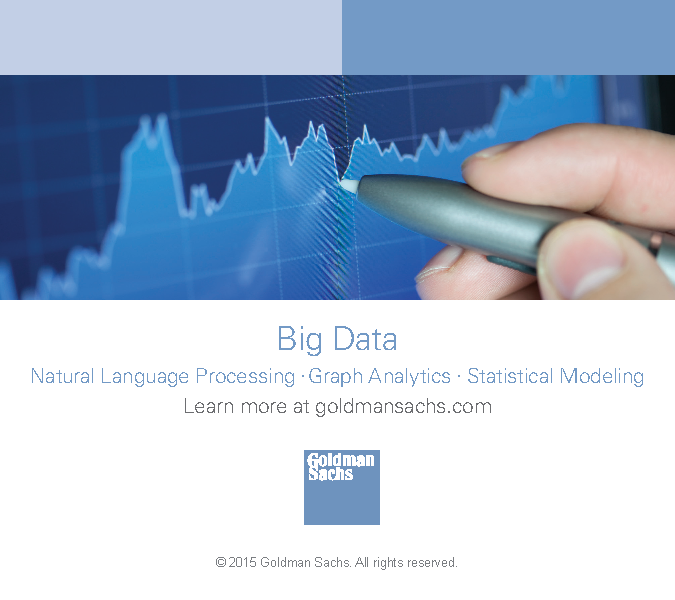
\includegraphics[width=4in]{content/ads/gold/goldman_sachs.pdf} \\
  %% SILVER %%%%%%%%%%%%%%%%%%%%%%%%%%%%%%%%%%%%%%%%%%%%%%%%%%%%%%%
  %
\includegraphics[width=4in]{content/ads/bronze/yahoo_labs.pdf} \\
  %
\includegraphics[width=4in]{content/ads/silver/sdl_research.pdf} \\
\end{tabular}
\end{center}

%% PLATINUM %%%%%%%%%%%%%%%%%%%%%%%%%%%%%%%%%%%%%%%%%%%%%%%%%%%%%
\clearpage
\thispagestyle{empty}
\begin{center}
  \vfill
  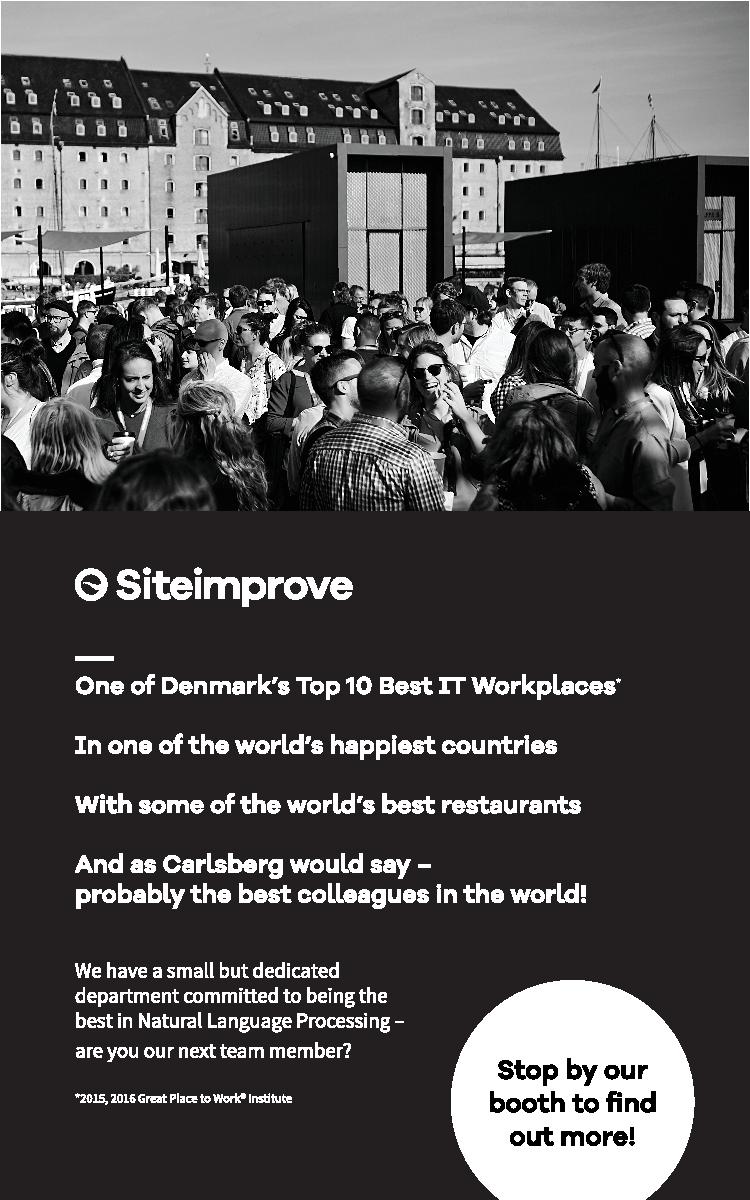
\includegraphics[width=4in]{content/ads/platinum/siteimprove.pdf}
  \vfill
\end{center}



\cleartobackcover
\clearpage
\pagestyle{empty}

\begin{center}
The EMNLP organizers gratefully acknowledge the support from the following sponsors.
\\
\vspace{3em}
%\\
\begin{tabular*}{\textwidth}{@{\extracolsep{\fill}} ccc }
  \multicolumn{3}{l}{\small\textbf Diamond}\\\hline\\[0.5mm]
   
\includegraphics[width=1in,trim={0 180 0 180 },clip]{content/sponsors/diamond/google-logo.png} 
&  
\includegraphics[width=1in,trim={0 180 0 180 },clip]{content/sponsors/diamond/facebook-logo.png} 
&  
\includegraphics[width=1in,trim={0 180 0 180 },clip]{content/sponsors/diamond/bloomberg-logo.png}
\\
\\ 
\includegraphics[width=1in,trim={0 180 0 180 },clip]{content/sponsors/diamond/ku-leuven-logo.png} 
&  
\includegraphics[width=1in,trim={0 180 0 180 },clip]{content/sponsors/diamond/salesforce-logo.png} 
\end{tabular*} \\
\begin{tabular*}{\textwidth}{@{\extracolsep{\fill}} ccc }
  \multicolumn{3}{l}{\small\textbf Platinum}\\\hline\\[0.5mm]
   
\includegraphics[width=1in,trim={0 180 0 180 },clip]{content/sponsors/platinum/amazon-logo.png} 
&  
\includegraphics[width=1in,trim={0 180 0 180 },clip]{content/sponsors/platinum/baidu-logo.png} 
&  
\includegraphics[width=1in,trim={0 180 0 180 },clip]{content/sponsors/platinum/grammarly-logo.png}
\\
\\ 
\includegraphics[width=1in,trim={0 180 0 180 },clip]{content/sponsors/platinum/jingdong-logo.png} 
&  
\includegraphics[width=1in,trim={0 180 0 180 },clip]{content/sponsors/platinum/naverlabs-europe-logo.png} 
&  
\includegraphics[width=1in,trim={0 180 0 180 },clip]{content/sponsors/platinum/visit_brussels-logo.png} 
\end{tabular*} \\

\begin{tabular*}{\textwidth}{@{\extracolsep{\fill}} ccc }
    \multicolumn{3}{l}{\small\textbf Gold}\\\hline\\[0.5mm]
   
\includegraphics[width=1in,trim={0 180 0 180 },clip]{content/sponsors/gold/cvte-stacked-logo.png} 
&  
\includegraphics[width=1in,trim={0 180 0 180 },clip]{content/sponsors/gold/ebay-logo.png} 
&  
\includegraphics[width=1in,trim={0 180 0 180 },clip]{content/sponsors/gold/microsoft-logo.png} 
\\
   
\includegraphics[width=1in,trim={0 180 0 180 },clip]{content/sponsors/gold/naverline-logo.png} 
&  
\includegraphics[width=1in,trim={0 180 0 180 },clip]{content/sponsors/gold/oracle-logo.png} 
&  
\includegraphics[width=1in,trim={0 180 0 180 },clip]{content/sponsors/gold/polyai-logo.png} 
\end{tabular*} \\

\begin{tabular*}{\textwidth}{@{\extracolsep{\fill}} cccc }
  \multicolumn{3}{l}{\small\textbf Silver}\\\hline\\[0.5mm]
   
\includegraphics[width=1in,trim={0 180 0 180 },clip]{content/sponsors/silver/huawei-logo.png} 
&  
\includegraphics[width=1in,trim={0 180 0 180 },clip]{content/sponsors/silver/duolingo-logo.png} 
&  
\includegraphics[width=1in,trim={0 180 0 180 },clip]{content/sponsors/silver/figure-eight-logo.png} 
&  
\includegraphics[width=1in,trim={0 180 0 180 },clip]{content/sponsors/silver/nuance-logo.png} 
\end{tabular*} \\

\begin{tabular*}{\textwidth}{@{\extracolsep{\fill}} ccc }
  \multicolumn{3}{l}{\small\textbf Bronze}\\\hline\\[0.5mm]
  
\includegraphics[width=1in,trim={0 180 0 180 },clip]{content/sponsors/bronze/next-canada-logo.png} 
& 
    & 
\end{tabular*} 
\end{center}


\end{document}

